\documentclass[a4paper,10pt]{article}
\usepackage[utf8]{inputenc}

% ----  Useful packages % ---- 
\usepackage{amsmath}
\usepackage{graphicx}
\usepackage{amsfonts}
\usepackage{amsthm}
\usepackage{amssymb}
% ----  Useful packages % ---- 

\usepackage{wrapfig}
\usepackage{caption}
\usepackage{subcaption}
\usepackage{hyperref}
\hypersetup{
    colorlinks,
    citecolor=black,
    filecolor=black,
    linkcolor=black,
    urlcolor=black
}

\graphicspath{ {./images/} }

% ---- Set page size and margins replace ------
\usepackage[letterpaper,top=2cm,bottom=2cm,left=3cm,right=3cm,marginparwidth=1.75cm]{geometry}
% ---- Set page size and margins replace ------

% ------- NOTA ------
\theoremstyle{remark}
\newtheorem{note}{Note}[subsection]
% ------- NOTA ------

% ------- OSSERVAZIONE ------
\theoremstyle{definition}
\newtheorem{observation}{Osservazione}[subsection]
% ------- OSSERVAZIONE ------

% ------- DEFINIZIONE ------
\theoremstyle{plain}
\newtheorem{definition}{Definizione}[subsection]
% ------- DEFINIZIONE ------

% ------- ESEMPIO ------
\theoremstyle{definition}
\newtheorem{example}{Esempio}[subsection]
% ------- ESEMPIO ------

% ------- DIMOSTRAZIONE ------
\theoremstyle{definition}
\newtheorem{demostration}{Dimotrazione}[subsection]
% ------- DIMOSTRAZIONE ------

% ------- TEOREMA ------
\theoremstyle{definition}
\newtheorem{theorem}{Teorema}[subsection]
% ------- TEOREMA ------

% ------- COROLLARIO ------
\theoremstyle{plain}
\newtheorem{corollaries}{Corollario}[theorem]
% ------- COROLLARIO ------

% ------- PROPOSIZIONE ------
\theoremstyle{plain}
\newtheorem{proposition}{Proposizione}[subsection]
% ------- PROPOSIZIONE ------

% ---- Footer and header ---- 
\usepackage{fancyhdr}
\pagestyle{fancy}
\fancyhf{}
\fancyhead[LE,RO]{A.A 2020-2021}
\fancyhead[RE,LO]{Analisi Matematica}
\fancyfoot[RE,LO]{\rightmark}
\fancyfoot[LE,RO]{\thepage}

\renewcommand{\headrulewidth}{.5pt}
\renewcommand{\footrulewidth}{.5pt}
% ---- Footer and header ---- 

% ----  Language setting ---- 
\usepackage[italian, english]{babel}
% ----  Language setting ---- 

\title{\textbf{Analisi Matematica}}
\author{Realizzato da: Giuntoni Matteo}
\date{A.A. 2021-2022}

\begin{document}
\tableofcontents
\newpage
\maketitle
\begin{center}
    \vspace{-20pt}
    \rule{11cm}{.1pt} 
\end{center}

\section{Introduzione}

\subsection{Insiemi Numerici}
Un insieme di numeri è una raccolta di elementi. Alcuni degli insiemi che verranno utilizzati maggiormente in questo corso sono:
\begin{itemize}
    \item \textbf{N. Naturali} cioè tutti gli interi non negativi: $\mathbb{N}$ = $\{0, 1, 2, 3, 4, ...\}$.
    \item \textbf{N. Interi} cioè tutti gli interi con segno qualsiasi: $\mathbb{Z} = \{..., -3, -2, -1, 0, 1, 2, 3, ...\}$.
    \item \textbf{N. Razionali}, cioè le frazioni: $\mathbb{Q} = \{\frac{p}{q}$ dove p e q $\in \mathbb{Z}$ e $q \neq 0\}$. \\
    Un sottoinsieme sono le \textbf{classi di equivalenza} che sono tutte le frazioni semplificate ai minimi termini. 
    \item \textbf{N. Reali}, che possono essere visti come tutti gli elementi rappresentabili su una retta: $\mathbb{R}$ 
\end{itemize}
\begin{note}
I vari insiemi si contengono fra di loro. ($\mathbb{N} \subset \mathbb{X} \subset \mathbb{Q} \subset \mathbb{R}$) 
\end{note}
\begin{note}
Esistono molti numeri reali che non sono razionali e non si possono scrivere come frazioni. E.g. $\sqrt{2}, \pi, ...$
\end{note}

\subsection{Intervalli}
\begin{definition}[Intervallo]
    Un sottoinsieme $I \subseteq \mathbb{R}$ è un intervallo se $\forall \: x,\:y \in I$ $\mid$ $x < y$ $\wedge$ $\forall z \mid x < z < y$ ho che $z \in I$. [\ref{fig:intervallo}]
\end{definition}
\begin{wrapfigure}{l}{7cm}
	\vspace{-20pt}
	\centering
	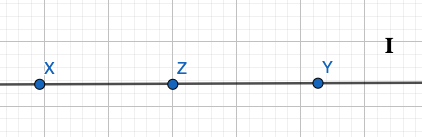
\includegraphics[width=5cm]{Intervallo.png}
	\caption{Tutto il segmento fra x e y deve stare in I}
	\label{fig:intervallo}
\end{wrapfigure}
I è un intervallo se ogni \emph{ogni} punto che prendo tra gli estremi dell'intervallo, questo appartiene all'intervallo stesso.
\\\\\\\\\\
\begin{example}
Esempi di intervalli.\\ \\
Questo caso \textbf{è un intervallo} \hspace{3.2cm} Questo caso \textbf{non è un intervallo} fra A e D.
\begin{figure}[h!]
    \vspace{-10pt}
    \begin{subfigure}{.5\textwidth}
        \hspace{-50pt}
        \centering
        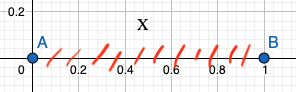
\includegraphics[width=6cm]{Esempio-intervallo-1.png}
        \caption{$A = \{x \in \mathbb{R} \: | \: 0<x<1\}$}
    \end{subfigure}
    \begin{subfigure}{.5\textwidth}
        \centering
        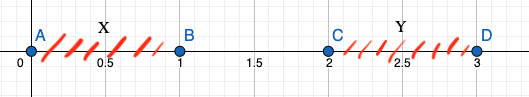
\includegraphics[width=7.5cm]{Esempio-intervallo-2.png}
        \caption{$C = \{x \in \mathbb{R} \: | \: 0<x<1 \: \vee \: z<x<3\}$}
    \end{subfigure}
\end{figure}
\end{example}

\newpage
\subsection{Notazione}
Con $a, b \in \mathbb{R}$ e con $a < b$ è possibile scrivere le notazioni in tabella \ref{tab:notazione-intervalli}.
\begin{table}[h!]
    \centering
    \setlength{\tabcolsep}{7pt}
    \renewcommand{\arraystretch}{2}
    \begin{tabular}{|c|c|c|} \hline
        [a, b] & Intervallo chiuso di estremi a e b & $\{x \in \mathbb{R} \: | \: a \leq x \leq b\}$ \\ \hline
        (a, b) & Intervallo aperto & $\{x \in \mathbb{R} \: | \: a < x < b\}$ \\ \hline
        [a, b) & Intervallo semi aperto a destra & $\{x \in \mathbb{R} \: | \: a \leq x < b\}$ \\ \hline
        (a, b] & Intervallo semi aperto a sinistra & $\{x \in \mathbb{R} \: | \: a < x \leq b\}$ \\ \hline
        [a, $+\infty$) & Semiretta chiusa a sinistra & $\{x \in \mathbb{R} \: | \: a \leq x\}$ \\ \hline
        ($-\infty$, b] & Semiretta chiusa a destra & $\{x \in \mathbb{R} \: | \: x \leq b\}$ \\ \hline
        ($-\infty$, $+\infty$) & Insieme di tutti i numeri $\mathbb{R}$ & $\{x \in \mathbb{R}\}$ \\ \hline
    \end{tabular}
    \caption{Notazione Intervalli}
    \label{tab:notazione-intervalli}
\end{table}
\newpage
\section{Funzioni}
\begin{definition}[Funzione]
- $f: A \longrightarrow B$: \\
Dati due insiemi A, B, detti corrispettivamente dominio e codominio, una funzione è una "legge" o "regola" che associa ad ogni elemento di $a \in A$ uno ed uno solo elemento di B, che si denota con f(a).
\end{definition}
\begin{note}
Tipicamente in questo corso le funzioni saranno date come formule del tipo $f(x) = x^2 - 7x - e^x$ andando poi a specificare dominio e codominio in questo modo $f: \mathbb{R} \longrightarrow \mathbb{R}$
\end{note}
\begin{example}
    Esempi funzioni:
    \begin{itemize}
        \item $g(x) = x^2 - 7x - e^x$ \hspace{.3cm} $g(0,+\infty) \longrightarrow \mathbb{R}$
        \item $g(x) = x^2$ \hspace{.3cm} $g(0, +\infty) \longrightarrow (0, +\infty)$. \hspace{.3cm}Va bene perché $x^2 > 0$ per qualsiasi valore di x.
        \item $h(x) = x^2$ \hspace{.3cm} $h(0, +\infty) \longrightarrow (-\infty, 0)$. \hspace{.3cm}Questa forma non va bene non definendo una funzione perché la formula non mi da numeri di $(-\infty, 0)$.
        \item $h(x) = x^2$ \hspace{.3cm} $h(0, +\infty) \longrightarrow (-\infty,1)$ \hspace{.3cm}Non va bene perché se preindiamo x=3 $f(3) = 9$ e 9 non fa parte del codominio. 
    \end{itemize}
\end{example}
Una funzione $f: A \longrightarrow B$ con $A,B \in \mathbb{R}$ ha un \textbf{grafico} che si indica come:
\begin{equation}
    graph(f) = \{(a,b) \in A \:X\: B\ \:|\: b = f(a)\}
\end{equation}
\begin{wrapfigure}[8]{l}{7cm}
    \centering
    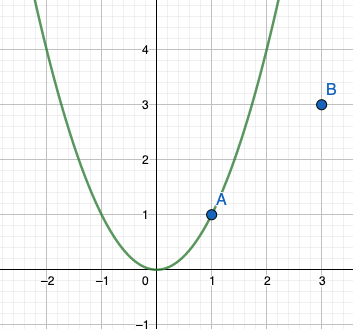
\includegraphics[width=4.5cm, height=4cm]{Esempio-grafico.png}
    \caption{$f(x) = x^2$ con $f: \mathbb{R} \longrightarrow \mathbb{R}$}
    \label{fig:esempio-grafico}
\end{wrapfigure}
\begin{example}
Esempio punto sulla funzione
\begin{itemize}
    \item Il punto A sta sul grafico si $f(x) = x^2$ esattamente quando $y = x^2$.
    \item Il punto B non sta sul grafico quindi $y \neq x^2$.
\end{itemize}
\end{example}
\begin{note}
    A X B $\subseteq \mathbb{R}$ X $\mathbb{R}$. Dove R X R = $R^2$.
\end{note}
\begin{example}
A e B = $(0, +\infty)$, da qui vediamo che A X B rappresenta il primo quadrante.\\\\
\end{example}

\subsection{Immagine}
\begin{definition}[Immagine]
Prendendo $f: A \longrightarrow B$ e $D \subseteq A$ l'immagine di D tramite f è il sottoinsieme $f(D) \subseteq B$ costituito dagli elementi f(d) dove $d \in D$.
\end{definition}
\begin{example}
    Esempi immagine:
    \begin{itemize}
        \item Immagine di A, $f(A) \subseteq B$ si chiama anche immagine della funzione.
        \item $f(x) = x^2$, $f: \mathbb{R} \longrightarrow \mathbb{R}$ \hspace{.2cm} immagine di g è $[0, +\infty)$ perché $x^2 \geq 0 \: \forall \: x \in \mathbb{R}$.
        \item $g(x) = x?2$, $g:[2, +\infty) \longrightarrow \mathbb{R}$ \hspace{.2cm} l'immagine di g è $[4, +\infty]$ perché se si calcola il punto minore del dominio, cioè 2, torna $g(2) = x^2$ che è uguale a 4, da lì possiamo prendere tutti i punti.
    \end{itemize}
\end{example}

\subsection{Suriettiva}
\begin{definition}[Suriettiva]
Una funzione si dice suriettiva quando ogni elemento del codominio è immagine di almeno un elemento del dominio. Quindi prendendo una f(x), per che sia suriettiva deve l'immagine I essere uguale ad un valore, $I(f) = b$.
\end{definition}
\begin{example}
    Esempi funzioni suriettive:
    \begin{itemize}
        \item $f(x) = x^2$, $f: \mathbb{R} \longrightarrow \mathbb{R}$ non è suriettiva perché tutti i valori del codominio $y < 0$ non hanno un rispettivo nel dominio.
        \item $g(x) = x^2$, $g: \mathbb{R} \longrightarrow (0, +\infty)$ lo è perchè andiamo a restringere il codominio ai punti che hanno un corrispettivo nel dominio.
    \end{itemize}
\end{example}

\subsection{Iniettiva}
\begin{definition}[Iniettiva]
Una funzione iniettiva è una funzione che associa, a elementi distinti del dominio, elementi distinti del codominio. Quindi prendendo una f(x) è iniettiva se prendendo due valori $x_1, x_2$ dove $x_1 \neq x_2 \Longrightarrow f(x_1) \neq f(x_2)$. (Input diversi danno output diversi).
\end{definition}
\begin{example}
    Esempi funzioni iniettiva:
    \begin{itemize}
        \item $f(x) = x^2$, $f: \mathbb{R} \longrightarrow \mathbb{R}$ non è iniettiva perché se prendiamo $x_1 = 1$ e $x_2 = -1$ $f(x1) = f(x2).$
        \item $g(x) = x^2$, $g: [0, +\infty) \longrightarrow \mathbb{R}$ è invece iniettiva perché non consideriamo i valori negativi.
    \end{itemize}
\end{example}

\subsection{Biunivoca}
\begin{definition}[Biunivoca]
Una funzione si definisce biunivoca o bigettiva se è sia iniettiva che suriettiva.
\end{definition}

\subsection{Invertibile}
\begin{definition}[Invertibile]
Se una funzione è biunivoca si dice che tale funzione è anche invertibile.
\end{definition}
\begin{wrapfigure}{l}{6cm}
    \centering
    \includegraphics[width=5cm, height=4cm]{Esempio-invertibilità.png}
    \caption{$f(x) = x^2$ e $g(x) = \sqrt{x}$}
    \label{fig:esempio-invertibilità}
\end{wrapfigure}
Se f è una funzione invertibile i grafici di f e di $f^i$ (la funzione inversa) sono simmetrici rispetto alla retta y=x cioè alla bisettrice del primo e del terzo quadrante. \\
\begin{example}
Se vediamo nell'immagine [\ref{fig:esempio-invertibilità}] prendendo l'inverso della funzione $f(x) = x^2$ definita in $[0, +\infty] \longrightarrow \mathbb{R}$ e cioè la funzione $g(x) = \sqrt{x}$ è simmetrica.
\\ \\ \\ \\ \\
\end{example}

\subsection{Funzioni Monotone}
\begin{definition}[Monotone]
Dato un insieme $A \in \mathbb{R}$ e $x_1, x_2 \in A$ con $x_1 < x_2$ se $\forall x_1, x_2$ risulta ciò che è scritto in Tabella \ref{tab:monotone}.
\end{definition}
\begin{table}[h!]
    \centering
    \setlength{\tabcolsep}{6pt}
    \renewcommand{\arraystretch}{1.7}
    \begin{tabular}{|c|c|}
        \hline
        \textbf{[1] Strettamente Crescente} & $f(x_1) < f(x_2) $ \\ \hline
        \textbf{[2]Debolmente Crescente} & $f(x_1) \leq f(x_2) $ \\ \hline
        \textbf{[3]Strettamente Decrescente} & $f(x_1) > f(x_2) $ \\ \hline
        \textbf{[4]Debolmente Decrescente} & $f(x_1) \geq f(x_2) $ \\ \hline
    \end{tabular}
    \caption{Definizioni funzioni crescenti e decrescenti}
    \label{tab:monotone}
\end{table}
Andando a considerare la Tabella \ref{tab:monotone} possiamo dire che:
\begin{itemize}
    \item \textbf{Strettamente monotona} nei casi [1] e [3] della tabella.
    \item \textbf{Debolmente monotona} nei casi [2] e [4] della tabella.
\end{itemize}

\begin{example}
    Esempi funzioni crescenti e decrescenti:\\
    \begin{figure}[h!]
        \begin{subfigure}{.5\textwidth}
            \centering
            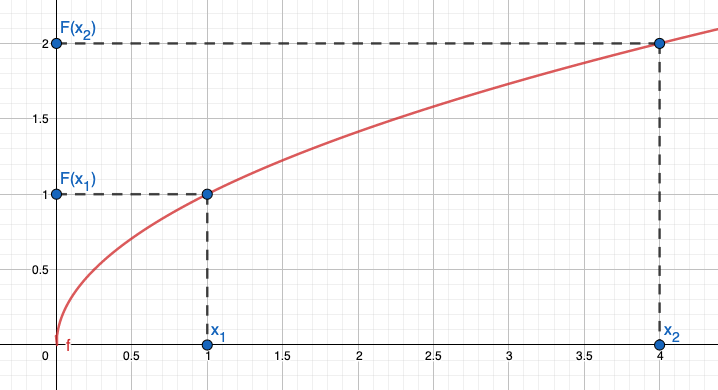
\includegraphics[width=6cm, height=4cm]{funzione-crescente.png}
            \caption{$f(x_1) < f(x-2)$ quindi è crescente}
            \label{fig:funzione-crescente}
        \end{subfigure}
        \begin{subfigure}{.5\textwidth}
            \centering
            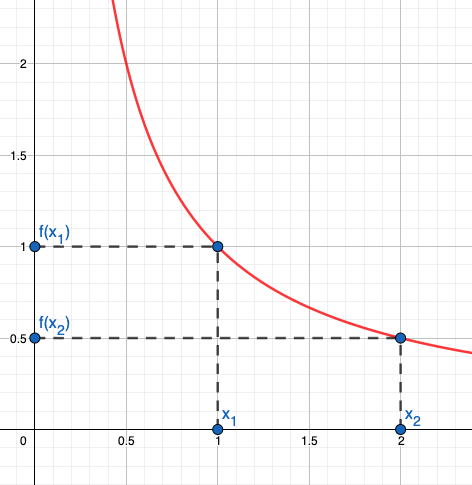
\includegraphics[width=6cm, height=4cm]{funzione-decrescente.png}
            \caption{$f(x_1) > f(x-2)$ quindi è decrescente}
            \label{fig:funzione-decrescente}
        \end{subfigure}
    \end{figure}
    \\Possiamo anche federe dalle immagini [\ref{fig:funzione-crescente}] [\ref{fig:funzione-decrescente}] che:
    \begin{itemize}
        \item Se f(x) è \textbf{crescente} l'ordinamene verrà \textbf{mantenuto}.
        \item Se f(x) è \textbf{decrescente} l'ordinamento verrà \textbf{invertito}.\\
    \end{itemize}
\end{example}

\begin{observation}
    Osservazione sul rapporto incrementale:\\
\end{observation}
\begin{wrapfigure}[8]{l}{8cm}
    \vspace{-15pt}
    \centering
    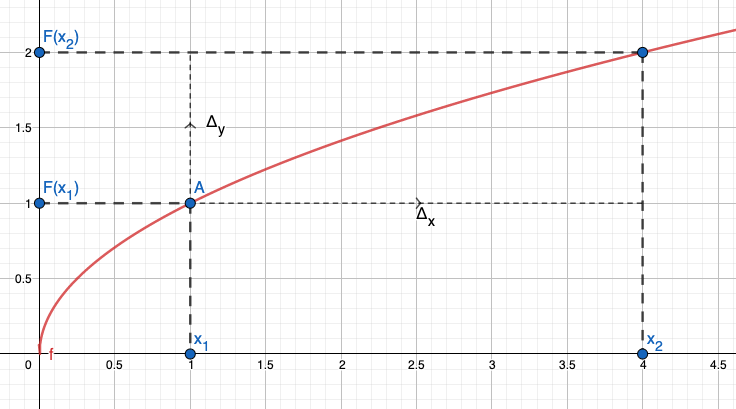
\includegraphics[width=6.7cm]{rapporto_incrementale.png}
    \caption{$\frac{\Delta_y}{\Delta_x}$}
    \label{fig:esempio-invertibilità}
\end{wrapfigure}
f(x) è strettamente crescente se e solo se il \textbf{rapporto incrementale}\footnote{I rapporto incrementale misura quanto il punto della f si sposta in verticale in rapporto a quanto abbiamo l'asciasse in orizzontale.} è maggiore di 0:
\begin{equation}
    \frac{f(x_1) - f(x_2)}{x_1 - x_2} > 0
\end{equation}
\begin{note}
    Il denominatore ed il numeratori devono essere concordi per fare in modo che il rapporto incrementale sia maggiore di 0 e quindi la funzione crescente. \\ \\\\
\end{note}
Continuando ad analizzare il rapporto incrementale possiamo ricavare anche i casi in cui una funzione e strettamente decrescente o debolmente crescente o debolmente decrescente. Puoi vedere tutte le casistiche nella tabella \ref{tab:analisi-rapporto-incrementale}.
\begin{table}[h!]
    \centering
    \setlength{\tabcolsep}{7pt}
    \renewcommand{\arraystretch}{2}
    \begin{tabular}{|c|c|}
        \hline
        Strettamente Crescente & $\frac{f(x_1) - f(x_2)}{x_1 - x_2} > 0$\\ \hline
        Strettamente Decrescente & $\frac{f(x_1) - f(x_2)}{x_1 - x_2} < 0$ \\ \hline
        Debolmente Crescente & $\frac{f(x_1) - f(x_2)}{x_1 - x_2} \geq 0$ \\ \hline
        Debolmente Decrescente & $\frac{f(x_1) - f(x_2)}{x_1 - x_2} \leq 0$ \\ \hline
    \end{tabular}
    \caption{Analisi rapporto incrementale}
    \label{tab:analisi-rapporto-incrementale}
\end{table}
\begin{observation}
    Se una funzione f(x) è strettamente crescente è a sua volta anche debolmente crescente, mentre una funzione f(x) se è debolmente crescente non è strettamente crescente perché aggiunge una casistica che sarebbe $f(x_1) = f(x_2)$. 
\end{observation}
\begin{example}
    Casistica particolare:\\
    Data $f(x)=\frac{1}{x}$, \hspace{.3cm} $f: \mathbb{R} \: \setminus \: \{0\} \longrightarrow \mathbb{R} \: \setminus \: \{0\}$. Funzione rappresentata nell'immagine [\ref{fig:esempio-particolare}].
    \begin{figure}[h!]
        \centering
        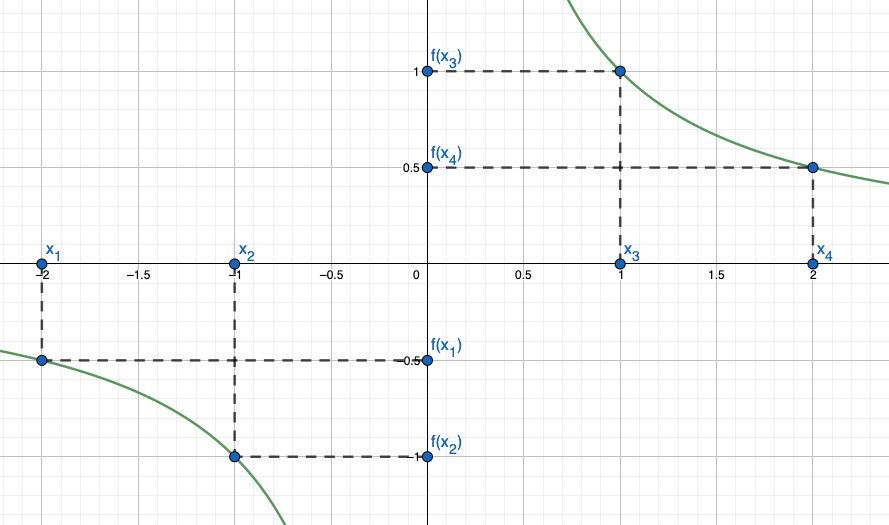
\includegraphics[width=8.7cm]{esempio-particolare.png}
        \caption{$f(x)=\frac{1}{x}$, \hspace{.3cm} $f: \mathbb{R} \: \setminus \: \{0\} \longrightarrow \mathbb{R} \: \setminus \: \{0\}$}
        \label{fig:esempio-particolare}
    \end{figure}
    \\Possiamo vedere che:
    \begin{itemize}
        \item f(x) è strettamente decrescente in $(0, +\infty)$.\\
        Quindi se andiamo a prendere $0 < x_3 < x_4$ abbiamo che $f(x_3) > f(x_4)$.
        \item f(x) è strettamente decrescente in $(-\infty, 0)$.\\
        Quindi se andiamo a prendere $x_1 < x_2 < 0$ abbiamo che $f(x_1) > f(x_2)$.
    \end{itemize}
    Se però andiamo a considerare tutto $\mathbb{R} \: \setminus \: \{0\}$, e quindi prendiamo i punti $x_1 < 0 < x_4$ vediamo che $f(x_1) < f(x_4)$.
    In conclusione si può dire quindi che $f(x)=\frac{1}{x}$) è decrescente in $(-\infty, 0)$ e in $(0, +\infty)$ ma non lo è in tutto $\mathbb{R} \: \setminus \: \{0\}$.
\end{example}

\subsubsection{Composizione con funzioni monotone}
\begin{note}
     Il simbolo della composizione è "$\circ$", come $f \circ g$.
\end{note}
Prendendo i considerazioni 3 insiemi A, B, C tali che $A, B, C \subset \mathbb{R}$ e 2 funzioni f(x) e g(x) così definitine: \hspace{.2cm} $f: A \longrightarrow B$, $g: B \longrightarrow C $.
\begin{enumerate}
    \item Se f è crescente e g è crescente allora $g \circ f$ è crescente.
    \item Se f è crescente e g è decrescente allora $g \circ f$ è decrescente. (Vale anche l'inverso).
    \item Se f è decrescente e g è decrescente allo $g \circ f$ è crescente. 
\end{enumerate}
\begin{example}
    $h(x) = e^{x^3}$\\
    La funzione h si ottiene dalla composizione di:
    \begin{itemize}
        \item $f: \mathbb{R} \longrightarrow \mathbb{R}$ \hspace{.3cm} $f(x) = x^3$. Funzione crescente.
        \item $g: \mathbb{R} \longrightarrow \mathbb{R}$ \hspace{.3cm} $g(t) = e^t$. Funzione decrescente.
    \end{itemize}
    Quindi possiamo scrivere $h(x) = e^{x^3}$ come: \hspace{.3cm} $e^{f(x)} \: \: = \: \: g(f(x)) \: \: = \: \: (g \circ f)(x)$
    Inoltre visto che f è crescente e g è crescente, h è strettamente crescente 
\end{example}
\begin{observation}
    Se prendiamo una funzione f(x) strettamente monotona, allora f(x) è iniettiva. Questa condizione è vera ma NON lo è viceversa: una funzione f(x) iniettiva NON è per forza strettamente monotona. 
\end{observation}
\begin{example}
    Se prendiamo una f(x) tale che: \hspace{.3cm} $f(x) = \frac{1}{x}$ \hspace{.3cm} $\mathbb{R} \setminus \{0\} \longrightarrow \mathbb{R} \setminus \{0\}$
    \\Possiamo vedere rifacendoci all'esempio in figura [\ref{fig:esempio-particolare}] che f è iniettiva ma non monotona.
\end{example}

\subsection{Insieme di definizione}
\begin{definition}[Insieme di definizione]
    Prendendo una funzione f(x) l'insieme di definizione o dominio naturale di una funzione è il più grande sottoinsieme di $\mathbb{R}$ dove ha senso la funzione f(x).
\end{definition}
\begin{example}
    $f(x) = \frac{1}{x}$ \hspace{.3cm} L'insieme di definizione è $\mathbb{R} \setminus \{0\}$
\end{example}

\subsection{Funzioni pari e dispari}
\begin{definition}[Pari]
    La funzione è \textbf{Pari} se $f(x) = f(-x) \: \forall x$ nel dominio di $f \longrightarrow f$.
\end{definition}
\begin{definition}[Dispari]
    La funzione è \textbf{Dispari} se $f(x) = -f(-x) \: \forall x$ nel dominio di $f \longrightarrow f$.
\end{definition}
\begin{note}
    Il dominio di f deve essere tale che se $x \in Dominio$ allora $-x \in Codominio$.\\
\end{note}
\begin{example}
Esempio funzioni pari e dispari.\\
\end{example}
$f(-x) = (-x)^2 = x^2 = f(x)$, f(x) è \textbf{pari}: \hfill $f(-x) = (-x)^2 = x^2 = -f(x)$, f(x) è \textbf{dispari}:
\begin{figure}[h!]
    \vspace{-1pt}
    \begin{subfigure}{.5\textwidth}
        \centering
        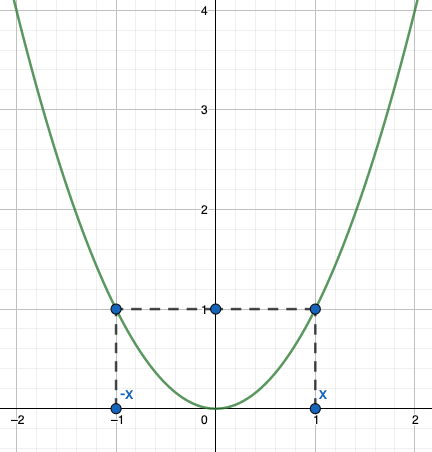
\includegraphics[width=3cm]{funzione-pari.png}
        \caption{$f(x) = x^2$, \hspace{.2cm} graph(f) con f pari}
    \end{subfigure}
    \begin{subfigure}{.5\textwidth}
        \centering
        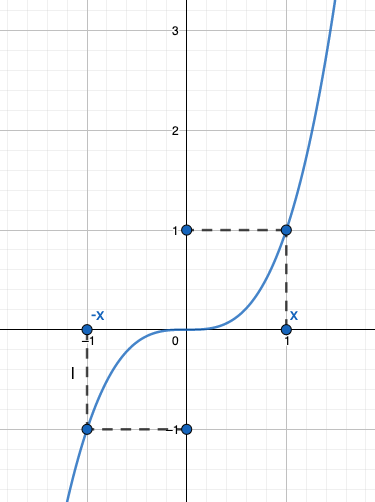
\includegraphics[width=2.5cm]{funzione-dispari.png}
        \caption{$f(x) = x^3$, \hspace{.2cm} graph(f) con f dispari}
    \end{subfigure}
\end{figure}

\subsection{Funzione periodica}
\begin{definition}[Periodicità]
    Una funzione f(x) si dice periodica di periodo $P \in \mathbb{R}$ se $\forall x \: \: f(x + P) = f(x)$. 
\end{definition}
\begin{wrapfigure}{r}{9cm}
    \vspace{-15pt}
    \centering
    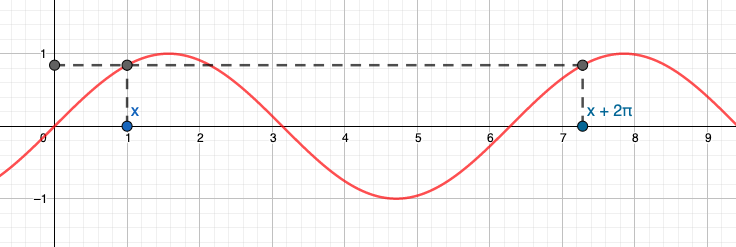
\includegraphics[width=7cm]{funzione-periodica.png}
    \caption{$sin(x) = sin(x + 2\pi)$}
    \label{fig:funzione-periodica}
\end{wrapfigure}
Inoltre il dominio di f(x) deve essere tale che $x \in$ Dominio è uguale e a $x + P \in$ codominio.
\begin{example}
In figura [\ref{fig:funzione-periodica}] un esempio di funzione periodica.\\\\
\end{example}

\newpage
\subsection{Funzioni Elementari}
\subsubsection{Retta}
\textbf{Funzione retta:} $f(x) = ax + b$. \hspace{.3cm} $a,b \in \mathbb{R}$ \\ Dove la "a" si dice coefficiente angolare, ed indica la pendenza della retta mentre la lettera "b" si chiama termine noto, ed indica il punto di incontro con l'asse Y.

\subsubsection{Esponente positivo o negativo}
\textbf{Fun. Esp. positivo:} $f(x) = x^k$, $k \in \mathbb{N}$. \hfill \textbf{Fun. Esp. negativo:} $f(x) = x^k$, $k \in \mathbb{N}$, $k < 0$.
\begin{figure}[h!]
    \begin{subfigure}{.5\textwidth}
        \centering
        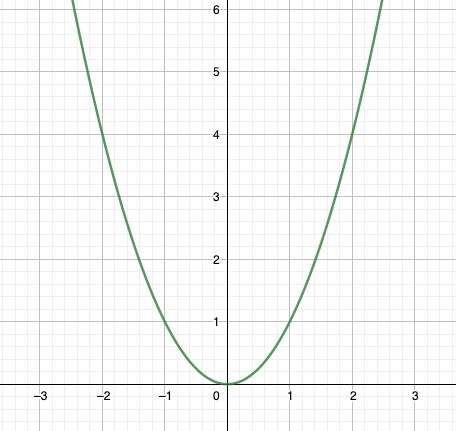
\includegraphics[width=4cm, height=3.5cm]{parabole.png}
        \caption{con k pari}
        \label{fig:esponente-positivo-pari}
    \end{subfigure}
    \begin{subfigure}{.5\textwidth}
        \centering
        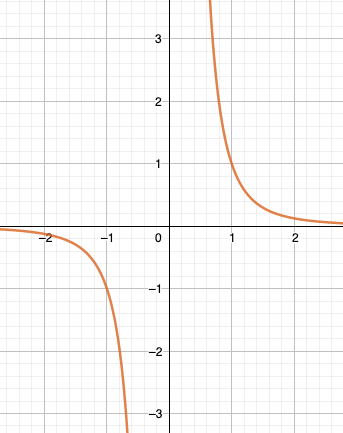
\includegraphics[width=4cm, height=3.5cm]{esponente-negativo-dispari.png}
        \caption{con k dispari}
        \label{fig:esponente-positivo-dispari}
    \end{subfigure}
\end{figure}
\begin{figure}[h!]
    \vspace{-5pt}
    \begin{subfigure}{.5\textwidth}
        \centering
        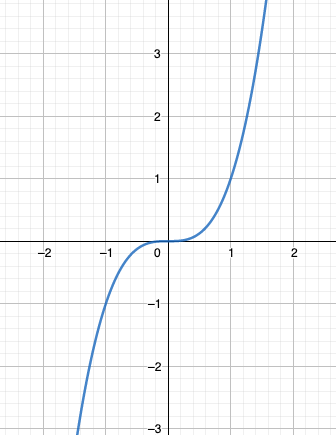
\includegraphics[width=4cm, height=3.7cm]{esponente-dispari.png}
        \caption{con k pari}
        \label{fig:esponente-negativo-pari}
    \end{subfigure}
    \begin{subfigure}{.5\textwidth}
        \centering
        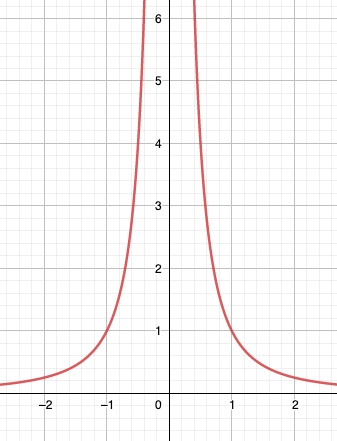
\includegraphics[width=4cm, height=3.5cm]{esponsente-negativo-pari.png}
        \caption{con k dispari}
        \label{fig:esponente-negativo-dispari}
    \end{subfigure}
\end{figure}
\begin{observation}
    \textbf{k pari:} Le funzioni con il k pari sono funzioni pari e hanno tutte una forma simile a quella in figura [\ref{fig:esponente-positivo-pari}] per le funzioni con k positive e per le funzioni con k negativo figura [\ref{fig:esponente-negativo-pari}].
\end{observation}
\begin{observation}
    \textbf{k dispari:} Le funzioni con il k positivo e dispari sono funzioni dispari e hanno tutte una forma simile a quella in figura [\ref{fig:esponente-positivo-dispari}] per le funzioni con k positive e per le funzioni con k negativo figura [\ref{fig:esponente-negativo-dispari}].
\end{observation}

\subsubsection{Radici o esponente fratto}
\textbf{Funzionane radici o esponente fratto:} $f(x) = x^{\frac{p}{q}}$ o $f(x) = \sqrt[q]{x^p}$  \: \: con  \: \:  $p, q \in \mathbb{N}$ \: \: e  \: \:  $q \neq 0$. \footnote{In matematica è possibile scrivere una un esponente fratto come radice mettendo il numeratore al radicando della radice e il denominatore all'indice: $x^{\frac{p}{q}} \: = \: \sqrt[q]{x^p}$}
\begin{figure}[h!]
    \begin{subfigure}{.5\textwidth}
        \centering
        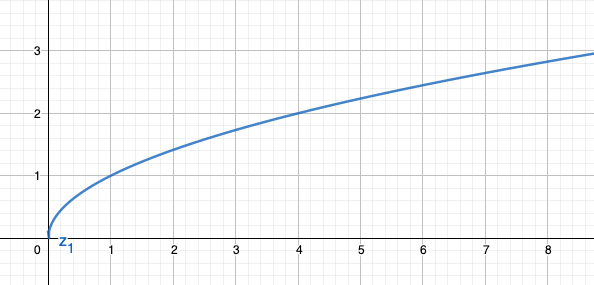
\includegraphics[width=6.3cm]{radice-pari.png}
        \caption{con q pari}
        \label{fig:radice-pari}
    \end{subfigure}
    \begin{subfigure}{.5\textwidth}
        \centering
        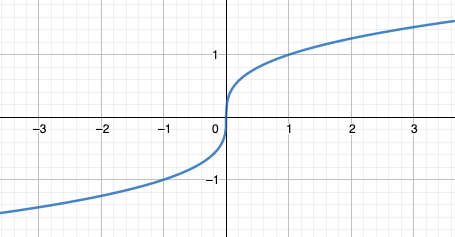
\includegraphics[width=6cm]{radice-dispari.png}
        \caption{con q dispari}
        \label{fig:radice-dispari}
    \end{subfigure}
\end{figure}
\begin{note}
    p e q non possono essere entrambi pari perché in tal caso sono divisibili fra di loro e quindi portabili ad una forma ridotta.
\end{note}
\begin{observation}
    \textbf{q pari:} Le funzioni con il q pari ha dominio $ x \geq 0$ ed è invertibile sono come funzione $f: [0, +\infty) \longrightarrow [0, +\infty)$. È rappresentata in figura [\ref{fig:radice-pari}].
\end{observation}
\begin{observation}
    \textbf{q dispari:} Le funzioni con il q positivo ha dominio $x \in \mathbb{R}$ ed è ugualmente invertibile su tutto $\mathbb{R}$, è inoltre una funzione dispari. È rappresentata in figura [\ref{fig:radice-dispari}].\\
\end{observation}

\subsubsection{Esponenziale}
\textbf{Funzione esponenziale:} $f(x) = a^x$ con $a \in \mathbb{R}$, \: \: $a > 0$, \: \: $a \neq 1$ \: \: $f: \mathbb{R} \longrightarrow (0, +\infty)$
\begin{figure}[h!]
    \begin{subfigure}{.5\textwidth}
        \centering
        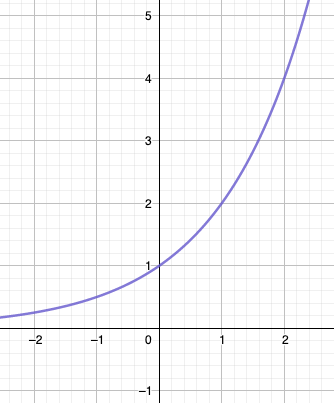
\includegraphics[width=4cm]{esponenziale.png}
        \caption{con $a > 1$}
        \label{fig:esponenziale}
    \end{subfigure}
    \begin{subfigure}{.5\textwidth}
        \centering
        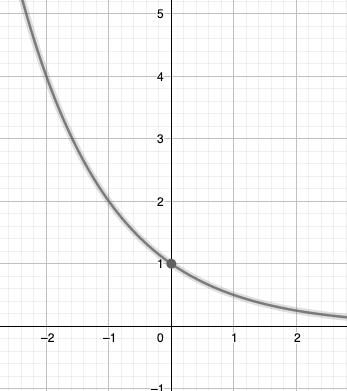
\includegraphics[width=4cm]{esponsenziale-base-minore.png}
        \caption{con $0 < a < 1$}
        \label{fig:esponsenziale-base-minore}
    \end{subfigure}
\end{figure}
\begin{note}
    La funzione esponenziale è sempre positiva.
\end{note}
\begin{observation}
    \textbf{$a > 1$:} La funzione è strettamente crescente, come in nell'immagine [\ref{fig:esponenziale}].
\end{observation}
\begin{observation}
    \textbf{$0 < a < 1$:} La funzione è decrescente, come in nell'immagine [\ref{fig:esponsenziale-base-minore}].
\end{observation}

\subsubsection{Logaritmo}
\textbf{Funzione logaritmo:} $f(x) = \log_a x$, \: \: $f: (0, +\infty) \longrightarrow \mathbb{R}$ \: \: (inversa dell'esponenziale).
\begin{figure}[h!]
    \begin{subfigure}{.5\textwidth}
        \centering
        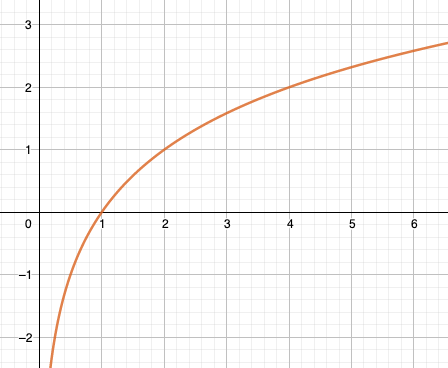
\includegraphics[width=5cm,height=4cm]{logaritmo.png}
        \caption{con $a > 1$}
        \label{fig:logaritmo}
    \end{subfigure}
    \begin{subfigure}{.5\textwidth}
        \centering
        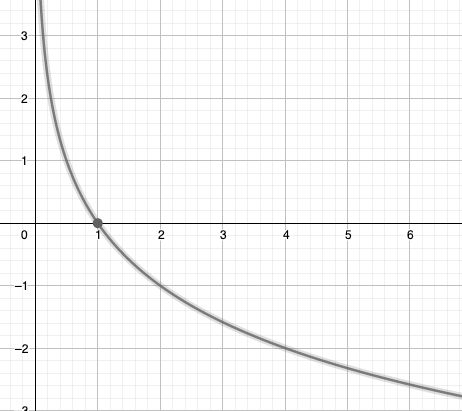
\includegraphics[width=5cm,height=4cm]{logaritmo-base-minore.png}
        \caption{con $0 < a < 1$}
        \label{fig:logaritmo-base-minore}
    \end{subfigure}
\end{figure}
\begin{observation}
    Casistica particolare - $f(x) = e^x$.\\
    In questa casistica se andiamo a ridurre il codominio la funzione esponenziale è invertibile. $f: \mathbb{R} \longrightarrow (0, +\infty)$.
    Il suo inverso è un caso particolare di logaritmo e di chiama \textbf{logaritmo naturale}. E si può scrive in due modi:
    \begin{itemize}
        \item $\ln{x}$: sarebbe logaritmo in base naturale.
        \item $\log x$: scrivendo il logaritmo senza la base intendiamo il logaritmo in base $e$.
    \end{itemize}
\end{observation}

\subsubsection{Seno e Arcoseno}
\textbf{Seno:} $f(x) = \sin x$, $f: \mathbb{R} \longrightarrow \mathbb{R}$. \hfill
\textbf{Arcoseno:} $f(x) = \arcsin x$, $f: [-1, 1] \longrightarrow [-\frac{\pi}{2}, \frac{\pi}{2}]$
\begin{figure}[h!]
    \begin{subfigure}{.5\textwidth}
        \centering
        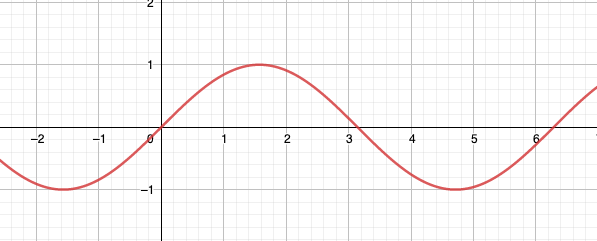
\includegraphics[width=6cm]{seno.png}
        \caption{$\sin{x}$}
        \label{fig:seno}
    \end{subfigure}
    \begin{subfigure}{.5\textwidth}
        \centering
        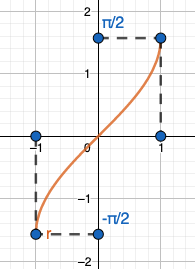
\includegraphics[width=2cm, height=2.3cm]{arcoseno.png}
        \caption{$\arcsin{x}$ o $\sin{x}^{-1}$}
        \label{fig:arcoseno}
    \end{subfigure}
\end{figure}

\begin{observation}
    \textbf{Sin(x):} La funzione $\sin{x}$ (immagine [\ref{fig:seno}]) è periodica per $2\pi$ quindi possiamo scrivere $\sin{(x+2\pi)} = \sin x \: \forall x \in \mathbb{R}$. Inoltre è suriettiva per codominio [-1, 1]. Se invece definiamo $f: [-\frac{\pi}{2}, \frac{\pi}{2}] \longrightarrow [-1, 1]$ la funzione $\sin x$ è strettamente crescente e suriettiva, quindi anche invertibile, e la sua inversa è appunto $\arcsin{x}$.
\end{observation}
\begin{observation}
    \textbf{Arcsin(x):} La funzione $\arcsin{x}$ è l'inverso del seno e può essere scritta anche come $f(x) = \sin{x}^{-1}$, è rappresentata nell'immagine [\ref{fig:arcoseno}].
\end{observation}

\subsubsection{Coseno e Arcocoseno}
\textbf{Coseno:} $f(x) = \cos{x}$, $f: \mathbb{R} \longrightarrow \mathbb{R}$. \hfill
\textbf{Arcocoseno:} $f(x) =\arccos{x}$, $f: [-1, 1] \longrightarrow [0, \pi]$
\begin{figure}[h!]
    \begin{subfigure}{.5\textwidth}
        \centering
        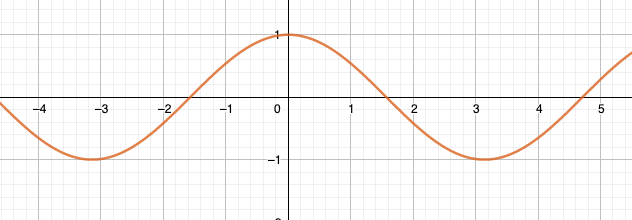
\includegraphics[width=6cm]{coseno.png}
        \caption{$\cos{x}$}
        \label{fig:coseno}
    \end{subfigure}
    \begin{subfigure}{.5\textwidth}
        \centering
        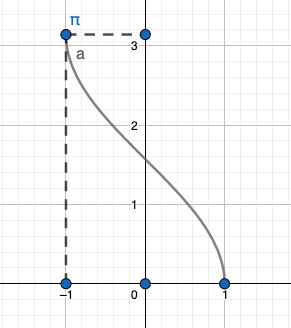
\includegraphics[width=3.5cm, height=2.7cm]{arcocoseno.png}
        \caption{$\arccos{x}$ o $\cos{x}^{-1}$}
        \label{fig:arcocoseno}
    \end{subfigure}
\end{figure}
\vspace{-5pt}
\begin{observation}
    \textbf{Cos(x):} La funzione $\cos{x}$, rappresentata nell'immagine [\ref{fig:coseno}], è periodica per $2\pi$ quindi possiamo scrivere $\cos{(x+2\pi)} = \cos x \: \forall x \in \mathbb{R}$. Inoltre è suriettiva per codominio [-1, 1]. Se invece definiamo $f: [0, \pi] \longrightarrow [-1, 1]$ la funzione $\cos x$ è suriettiva, quindi anche invertibile, e la sua inversa è appunto $\arccos{x}$.
\end{observation}
\begin{observation}
    \textbf{Arccos(x):} La funzione $\arccos{x}$ è l'inverso del seno e può essere scritta anche come $f(x) = \cos{x}^{-1}$ ed è rappresentata nell'immagine [\ref{fig:arcocoseno}].
\end{observation}

\subsubsection{Tangente e Arcotangente}
\textbf{Tangente:} $f(x) = \tan{x}$, $f: \mathbb{R} \longrightarrow \mathbb{R}$ \hfill
\textbf{Arcotangente:} $f(x) = \arctan{x}$, $f: \mathbb{R} \longrightarrow [-\frac{\pi}{2}, \frac{\pi}{2}]$
\begin{figure}[h!]
    \begin{subfigure}{.5\textwidth}
        \vspace{-20pt}
        \centering
        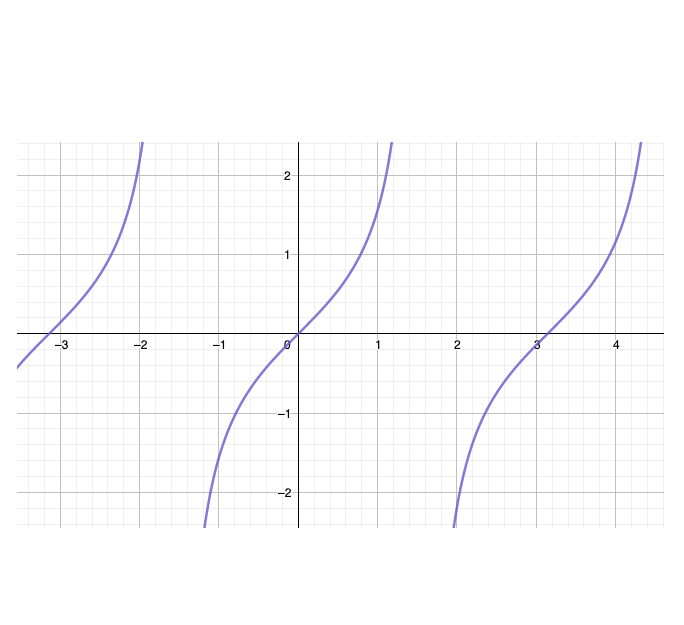
\includegraphics[width=4.2cm]{tangente.png}
        \vspace{-20pt}
        \caption{$\tan{x}$}
        \label{fig:tangente}
    \end{subfigure}
    \begin{subfigure}{.5\textwidth}
        \centering
        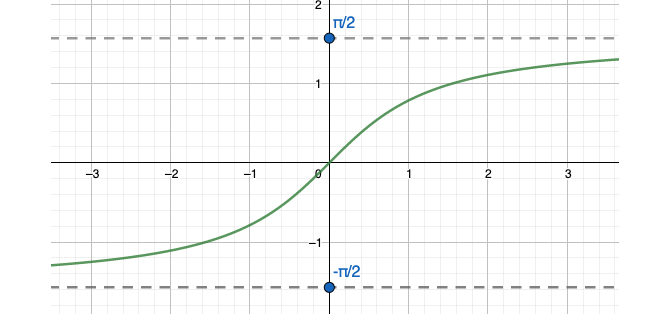
\includegraphics[width=5cm]{arcotangente.png}
        \caption{$\arctan{x}$ o $\tan{x}^{-1}$}
        \label{fig:arcotangente}
    \end{subfigure}
\end{figure}
\begin{observation}
    \textbf{Tan(x):} La funzione $\tan{x}$, rappresentata nell'immagine [\ref{fig:tangente}], può essere scritta anche come $\frac{\sin{x}}{\cos{x}}$, ha come dominio $\{x \in \mathbb{R} \: | \:  x \neq \frac{\pi}{2} + k\pi, \: k \in \mathbb{Z}\}$. La funzione tangente è fatta da infiniti intervalli, è quindi periodica per $\pi$; è di base non invertibile, ma se la ristringiamo in $f: [-\frac{\pi}{2}, \frac{\pi}{2}] \longrightarrow \mathbb{R}$ diventa biunivoca ed accetta la funzione inversa che è $\arctan{x}$.
\end{observation}
\begin{observation}
    \textbf{Arctan(x):} La funzione $\arctan{x}$, rappresentate nell'immagine [\ref{fig:arcotangente}], è inversa della funzione $\tan{x}$, può quindi essere scritta anche con la forma $\tan{x}^{-1}$.
\end{observation}
\section{Massimi e minimi}
\subsection{Massimo e minimo intervalli}
\begin{definition}[Massimo]
Dato un insieme A tale che: \\$A \subseteq \mathbb{R}, \: A \neq \O, \: m \in \mathbb{R}$ m si dice \textbf{massimo} di A se $m \geq a \: \forall \: a \in A$ e $m \in A$
\end{definition}
\begin{definition}[Minimo]
Dato un insieme A tale che: \\$A \subseteq \mathbb{R}, \: A \neq \O, \: m \in \mathbb{R}$ m si dice \textbf{minimo} di A se $m \leq a \: \forall \: a \in A$ e $m \in A$
\end{definition}
\begin{example}
    Esempi massini e minimi intervalli:
    \begin{itemize}
        \item Dato $A = [0,1]$ il max(A) = 1 e il suo min(A) = 0
        \item Dato $B = [0, 1)$ il min(B) = 0 mentre B non ha massimo.
    \end{itemize}
\end{example}

\begin{wrapfigure}{r}{8cm}
    \vspace{10pt}
    \centering
    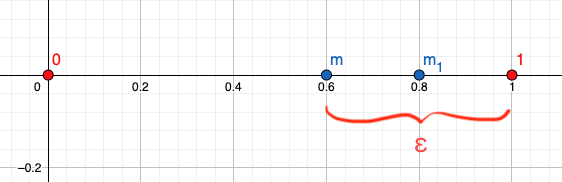
\includegraphics[width=7cm]{dimostrazione-massimo.png}
    \caption{Segmento B}
\end{wrapfigure}
\begin{demostration}
Dimostriamo questo esempio:
\end{demostration}
Supponiamo per assurdo che $m \in \mathbb{R}$ sia il max di B, con ovviamente $m \in B$. Se tale condizione è vera $m < 1$ perché 1 non è incluso nell'insieme B = [0, 1).\\ \\
Poniamo ora $\epsilon = 1 - m$, così facendo $\epsilon$ diventa la lunghezza dell'intervallo fra 1 ed m.\\ \\
Definiamo ora un $m_1 = m + \frac{\epsilon}{2}$. Creando questo valore $m_1$ vediamo che $m_1 \in B$ ma anche che $m < m_1$ che contrasta con la definizione di massimo di B che dovrebbe essere $m \geq b \: \forall \: b \in B$. Così dimostriamo la non esistenza di un valore massimo.

\subsection{Maggiorante e minorante intervalli}
\begin{definition}[Maggiorante]
$A \subseteq \mathbb{R}$, $A \neq \O$, $k \in \mathbb{R}$ si dice \textbf{maggiorante} di A se $k \geq a \: \: \forall \: \: a \in A$. L'insieme di tutti i maggioranti si indica con $M_A$.
\end{definition}
\begin{definition}[Minorante]
$A \subseteq \mathbb{R}$, $A \neq \O$, $k \in \mathbb{R}$ si dice \textbf{minorante} di A se $k \leq a \: \: \forall \: \: a \in A$. L'insieme di tutti i minoranti si indica con $m_A$.
\end{definition}
\begin{example}
A = [0,3] allora 3 è un maggiorante di A, quindi $3 \in M_A$. \\
Mentre $\frac{1}{4}$ non è un maggiorante, quindi $\frac{1}{4} \notin M_A$, perché $1 > A$ e $1 > \frac{1}{2}$.
\end{example}
\begin{observation}
    Se esiste un maggiorante di A allora ne esistono infiniti. Infatti se prendiamo un $k \in M_A$, m è un maggiorante di A $\forall \: \: m \geq k$.
    Questo discorso vale anche per i minoranti, infatti con $k \in m_A$, m è un minorante di A $\forall \: \: m \leq k$.
    \begin{example}
        Esempi per l'osservazione sopra:
        \begin{itemize}
            \item A = $\mathbb{R}$, A non ha maggioranti.
            \item A = [4, $+\infty$] non ha maggioranti ma ha minoranti.
        \end{itemize}
    \end{example}
\end{observation}

\subsection{Intervallo limitato}
\begin{definition}[Limitato superiormente]
    Dato un intervallo A, se $M_A \neq \O$ (insieme dei maggioranti) allora l'intervallo A si dice \textbf{limitato superiormente}
\end{definition}
\begin{definition}[Limitato inferiormente]
    Dato un intervallo A, se $m_A \neq \O$ (insieme dei minoranti) allora l'intervallo A si dice \textbf{limitato inferiormente}
\end{definition}
\begin{definition}[Limitato]
    $A \subset \mathbb{R}$, $A \neq \O$, se A è sia superiormente che inferiormente limitato allora A si dice semplicemente intervallo \textbf{limitato}.
\end{definition}
\begin{observation}
    A è limitato se e solo se $\exists \: \: h,k \in \mathbb{R}$ tale che $k \leq a \leq h \: \: \forall \: \: a \in A$
\end{observation}

\subsubsection{Estremi superiori ed inferiori}
\begin{theorem}[Estremo superiore]
    $A \subset \mathbb{R}$, $A \neq \O$ ed A è superiormente limitato, allora esiste il minimo dell'insieme dei maggioranti. Tale minimo si dice \textbf{estremo superiore} di A e si indica con sup(A).
\end{theorem}
\begin{theorem}[Estremo inferiore]
    $A \subset \mathbb{R}$, $A \neq \O$ ed A è inferiormente limitato, allora esiste il massimo dell'insieme dei minoranti. Tale massimo si dice \textbf{estremo inferiore} di A e si indica con inf(A).
\end{theorem}
\begin{example}
    Esempio estremi superiori ed inferiori:
    \begin{itemize}
        \item A = [0, 1) \hspace{.1cm} $M_A$ = [1, $+\infty$) e $m_A$ = ($-\infty$, 0] \hspace{.1cm} min($M_A$) = sup(A) = 1 \hspace{.2cm} max($m_A$) = inf(A) = 0
        \item B = [0, 1] \hspace{.1cm} $M_B$ = [1, $+\infty$) e $m_A$ = ($-\infty$, 0] \hspace{.1cm} min($M_B$) = sup(B) = 1 \hspace{.2cm} max($m_B$) = inf(B) = 0
    \end{itemize}
    \begin{observation}
        Se esiste max(A) allora max(A) = sup(A) e viceversa se esiste min(A) allora min(A) = inf(A)
    \end{observation}
\end{example}
\begin{note}
    Se A non è superiormente limitato scriviamo sup(A) = $-\infty$ e se non è inferiormente limitato inf(A) = $-\infty$.
\end{note}
\begin{observation}
    $A \neq \O$ e A è superiormente limitata, allora m = sup(A) se e solo se valgono 2 condizioni:
    \begin{enumerate}
        \item $a \leq m \: \: \forall \: \: a \in A$ \hspace{.3cm} Questo dice che m è un maggiorante
        \item $\forall \: \: \epsilon > 0 \: \: \exists \: \: \overline{a}$\footnote{$\overline{a}$ è un semplice metodo di notazione}$\in A \: \: | \: \: \overline{a} > m - \epsilon$ \hspace{.3cm} $m - \epsilon$ mi dice che non ci sono maggioranti più piccoli di m. 
    \end{enumerate}
    Se valgono queste 2 condizioni m è l'estremo sup e viceversa se m è sup(A) allora valgono queste condizioni.
    \begin{note}
        Questa considerazione vale anche per m = inf(A).
    \end{note}
\end{observation}
\begin{observation}
    La scrittura sup(A) $< +\infty$ vuol dire che l'estremo superiore di A è un numero reale, quindi A è superiormente limitato. Viceversa la scrittura inf(A) $> -\infty$ vuol dire che l'estremo inferiore di A è un numero reale, quindi A è inferiormente limitato.
\end{observation}

\subsection{Retta reale estesa}
\begin{definition}[Retta reale estesa]
    La retta reale estesa si indica con $\overline{\mathbb{R}} = \mathbb{R} \cup \{-\infty\} \cup \{+\infty\}$ in modo che valga: $-\infty \leq x \leq +\infty \: \: \forall x \in \overline{\mathbb{R}}$
\end{definition}
\begin{observation}
    Se $x \in \mathbb{R}$ (quindi $x \neq +\infty, x \neq -\infty$) allora $-\infty < x < +\infty$
\end{observation}

\subsubsection{Operazioni in $\overline{\mathbb{R}}$}
\begin{itemize}
    \item Se $x \neq +\infty$ allora $x + (-\infty) = -\infty$.
    \item Se $x \neq -\infty$ allora $x + (+\infty) = +\infty$.
    \item Se $x > 0$ allora $x(+\infty) = +\infty$ e $x(-\infty) = -\infty$.
    \item Se Se $x < 0$ allora $x(+\infty) = -\infty$ e $x(-\infty) = +\infty$.
    \item $(+\infty) + (-\infty)$ e viceversa \hspace{.3cm} $0(+\infty)$ o $0(\infty)$ \hspace{.3cm}\textbf{Sono vietate}
    \item $(+\infty)(+\infty) = +\infty$ \hspace{.2cm} $(+\infty)(-\infty) = -\infty$ \hspace{.2cm} $(-\infty)(-\infty) = +\infty$ \hspace{.2cm} \textbf{Sono consentite}
\end{itemize}
\begin{observation}
    Dato $A \subset \mathbb{Z}$ se A è superiormente limitato, A ha un massimo e se A è inferiormente limitato allora A ha un minimo.
\end{observation}

\subsection{Parte intera di un numero}
\begin{definition}
    Dato $x \in \mathbb{R}$ si dice \textbf{parte intera di x} e si indica con [x] il numero [x] = max$\{m \in \mathbb{Z}: m \leq x\}$
\end{definition}
\begin{wrapfigure}{r}{6cm}
    \vspace{-15pt}
    \centering
    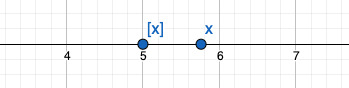
\includegraphics[width=5cm]{parte-intera.png}
    \caption{Parte intera di x}
    \label{fig:my_label}
\end{wrapfigure}
Possiamo spiegarlo in maniera semplice che è il primo numero intero che troviamo alla sinistra di x.
\begin{example}
    $[\frac{25}{10}] = 2$ \hspace{.5cm} $[-\frac{25}{10}] = -2$\\ \\
\end{example}

\vspace{-20pt}
\subsubsection{Grafico di f(x) = [x]}
\begin{wrapfigure}[8]{l}{7cm}
    \vspace{-25pt}
    \centering
    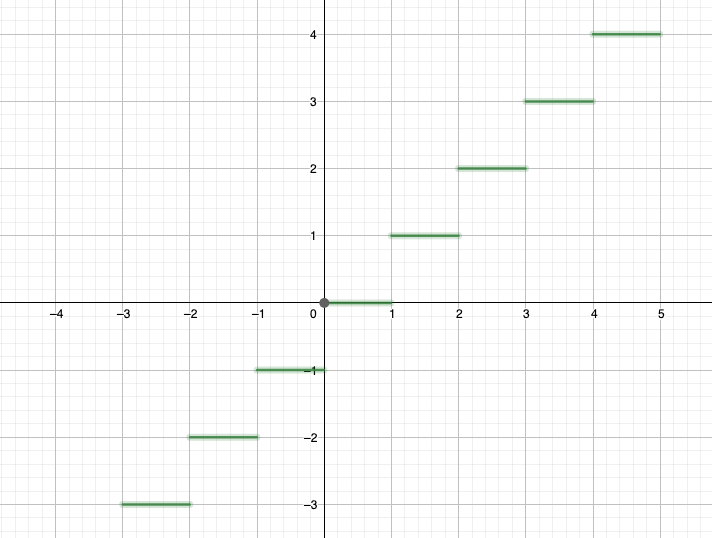
\includegraphics[width=5cm]{funzione-parte-intera.png}
    \caption{Grafico f(x) = [x]}
    \label{fig:funzione-parte-intera}
\end{wrapfigure}
\vspace{20pt}
Possiamo vedere nell'immagine [\ref{fig:funzione-parte-intera}] che tutti numeri vanno a valere in y come il valore del primo intero a sinistra.
\begin{example}
    Esempio per f(x) = [x]:\\
    $f(\frac{1}{2}) = 0$ \hspace{.3cm} $f(\frac{3}{2}) = 1$\\ \\
    $f(\frac{10}{3}) = 3$ \hspace{.3cm} $f(\frac{4}{3}) = 1$\\ \\ \\
\end{example}

\subsection{Limiti, massimi e minimi su funzioni}
Andiamo a fare una serie di definizioni prendendo due insiemi A, B tale che $A \subseteq \mathbb{R}$ e $B \subseteq \mathbb{R}$ ed una funzione $f(A)$ definita come $f: A \longrightarrow B$.
\begin{definition}[Limitata superiormente, inferiormente]
    $f$ si dice limitata superiormente se $f(A)$ è limitata superiormente. Viceversa $f$ si dice limitata inferiormente se $f(A)$ è limitata inferiormente. Se $f$ è sia limitata superiormente che inferiormente si dice che $f$ è limitata.
\end{definition}
\begin{definition}[Massimo e minimo]
    $f$ ha massimo se la sua immagine $f(A)$ ha massimo. Si dice che $M$ è il massimo di $f$ e si scrive $M = max(f)$ se $M = max(f(A))$. Ugualmente $f$ ha minimo se la sua immagine $f(A)$ ha minimo. Si dice che $m$ è il minimo di $f$ e si scrive $m = min(f)$ se $m = min(f(A))$.
\end{definition}
\begin{definition}
    Se f non è limitata superiormente e si scrive $sup(f) = +\infty$. Ugualmente se f non è limitata inferiormente, e si scrive $inf(f) = -\infty$.
\end{definition}
\begin{note}
    Rircoda che sup($f$) corrisponde a scrivere sup($f(A)$) e ugualmente inf($f$) è uguale a inf($f(A)$).
\end{note}
\begin{definition}[Punti di massimo e minimo]
    Se $f$ ha massimo allora ogni $x_0 \in A$ tale che $f(x_0) = max(f)$ si dice punto di massimo per $f$. Similmente se $f$ ha minimo allora ogni $x_0 \in A$ tale che $f(x_0) = min(f)$ si dice punto di minimo per $f$.
\end{definition}
\begin{observation}
    Il massimo di $f$ è unico mentre i punti di massimo possono essere molti.
\end{observation}

\begin{example}
    $f: \mathbb{R} \longrightarrow \mathbb{R}$ \hspace{.3cm} $f(x) = \sin{x}$ [\ref{fig:massimo_sinx}]
\end{example}
max(f) = 1 \hspace{.3cm} $x_0 = \frac{\pi}{2} + 2k\pi, k \in \mathbb{Z}$\\
\begin{wrapfigure}[4]{r}{8cm}
    \vspace{-45pt}
    \centering
    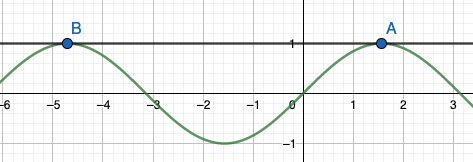
\includegraphics[width=6.5cm]{images/massimo_es1.png}
    \caption{funzione $f(x) = \sin{x}$}
    \label{fig:massimo_sinx}
\end{wrapfigure}
In questo caso essendo la funzione periodica in ogni intervallo di $x_0 = \frac{\pi}{2} + 2k\pi, k \in \mathbb{Z}$ esisterà un punto di massimo mentre il massimo rimarrà sempre 1.
\begin{example}
    $f:(0, +\infty) \longrightarrow \mathbb{R}$ \hspace{.3cm} $f(x) = \frac{1}{x}$ [\ref{fig:massimo-minimo-frazione}]
\end{example}
In questa casistica $f$ non ha ne massimo ne minimo. Questo lo possiamo dimostrare andando ad immaginare una casistica dove esiste un massimo ed un minimo e facendo poi alcune considerazione. \\
\begin{wrapfigure}{r}{6cm}
    \vspace{-15pt}
    \centering
    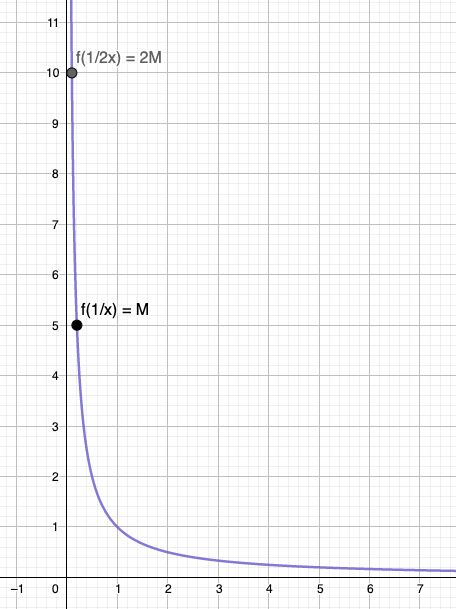
\includegraphics[width=4.5cm]{images/massimo_es2.png}
    \caption{funzione $f(x) = \frac{1}{x}$}
    \label{fig:massimo-minimo-frazione}
\end{wrapfigure}
Innanzitutto prendiamo per assurdo che $f$ avesse massimo allora $\Longrightarrow \: \: \exists \: \: m$ tale che $f(x) \leq m \: \: \forall \: \: x \in (0, +\infty)$. \\ Se in questa casistica prendessimo un punto x e dicessima che quello è il massimo, $f(\frac{1}{x}) = m$, ma se poi prendiamo un punto che è $\frac{x}{2}$ esso apparitene sempre alla funzione e $f(\frac{x}{2}) = 2m$ e $2m > m$. Quindi vediamo come non è possibile determinare un massimo.\\ \\
Questa funzione non può nemmeno avere un minimo perché $f(x) > 0 \: \: \forall \: \: x$, quindi $inf(f) = 0$. Se $f$ avesse minimo dovrebbe essere $m(f) = inf(f) = 0$ ma questo presuppone che debba esiste un $x_0$ tale che $f(x_0) = 0$ cioè $\frac{1}{x_0} = 0$, ma questo è impossibile.\\
\begin{observation}
    Consideriamo un insieme A $\subset \mathbb{R}$ e una funzione $f: A \longrightarrow \mathbb{R}$, valgono per essi le seguenti osservazioni:
    \begin{itemize}
        \item Se A ha massimo e $f$ è debolmente crescente allora $f$ ha max e max($f$) = $f$(max(A)).
        \item Se A ha minimo e $f$ è debolmente crescente allora $f$ ha min e min($f$) = $f$(min(A)).
        \item Se A ha minimo e $f$ è debolmente crescente allora $f$ ha min e min($f$) = $f$(max(A)).
        \item Se A ha massimo e $f$ è debolmente crescente allora $f$ ha max e max($f$) = $f$(min(A)).
    \end{itemize}
\end{observation}
\begin{figure}[h!]
    \begin{subfigure}{.5\textwidth}
        \centering
        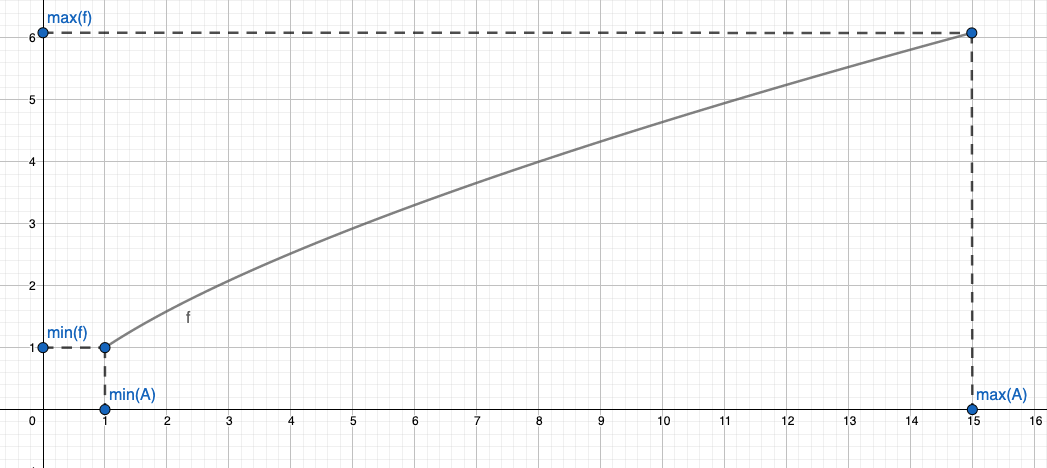
\includegraphics[width=6cm]{images/crescente-max-min.png}
        \caption{Punti max e min $f$ crescente}
        \label{fig:my_label}
    \end{subfigure}
    \begin{subfigure}{.5\textwidth}
        \centering
        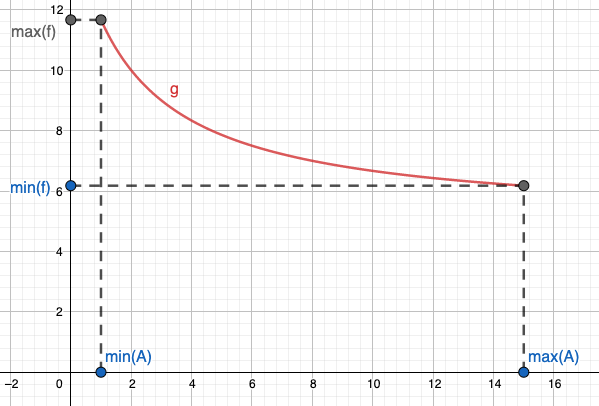
\includegraphics[width=4cm]{images/descrescente-max-min.png}
        \caption{Punti max min $f$ decrescente}
        \label{fig:my_label}
    \end{subfigure}
\end{figure}
\begin{observation}
    Se $f: A \longrightarrow \mathbb{R}$ allora m = sup($f$) se e solo se valgono queste due condizioni:
    \begin{enumerate}
        \item $f(x) \leq m \: \: \forall \: \: x \in A$ \hspace{.3cm} Questo vuol dire che m deve essere maggiore o uguale di qualsiasi f(x)
        \item $\forall \: \: \epsilon > 0 \: \: \exists \: \:  \overline{x} \in A \: \: | \: \: f(\overline{x}) > m - \epsilon$ \hspace{.3cm} Questo vuol dire che per qualsiasi valore $\epsilon$ maggiore di 0 deve esistere un $\overline{x}$ appartenendo all'insieme A tale che, se sottraiamo il valore $\epsilon$ a m il risultato deve essere inferiore a $f(\overline{x})$ ciò vuol dire che non ci sono altri valori per il quale la funzione è sempre sotto.
    \end{enumerate}
\end{observation}

\newpage
\section{Valore assoluto}
\begin{definition}[Valore assoluto]
    Dato $x \in \mathbb{R}$ si dice valore assoluto di x il massimo valore fra x e -x e si indica con $|x|$.
    \begin{equation}
        |x| = max(\{x, -(x)\})
    \end{equation}
\end{definition}
\begin{example}
    Esempi valore assoluto:
    \begin{itemize}
        \item $|5| = max(\{5, -5\}) = 5$
        \item $|-3| = max(\{-3, -(-3)\}) = 3$
    \end{itemize}
\end{example}
\subsection{Proprietà valore assoluto}
\begin{table}[h!]
    \setlength{\tabcolsep}{7pt}
    \renewcommand{\arraystretch}{2}
    \centering
    \begin{tabular}{|c|c|}
        \hline
        (1) $x \leq |x| \: \: \forall \: \: x \in \mathbb{R}$ & (2) $|x| = x$ se $x \geq 0, |x| = -x$ se $x \leq 0$ \\
        (3) $|x| \geq 0 \: \: \forall \: \: x \in \mathbb{R}$ & (4) $|x| = 0 \Longleftrightarrow x = 0$ \\
        (5) $|-x| = |x|$ & (6) $-|x| \leq x \leq |x|$ \\
        (7) $|x| \leq M \Longleftrightarrow -M \leq x \leq M$ con $M \geq 0$ & (8) $|x| \geq M \Longrightarrow x \geq M$ oppure $x \leq -M$ \\ \hline
    \end{tabular}
    \caption{Proprietà valore assoluto}
    \label{tab:prop-valore-assoluto}
\end{table}
\subsubsection{Spiegazioni proprietà}
Se stabiliamo un punto M maggiore del valore assoluto la funzione si troverà compreso fra M e -M. Se invece stabiliamo un punto M minore del valore assoluto la funzione sarà maggiore di M e minore di -M. Spiegazione grafica nell'immagine [\ref{fig:prop-6-7}]
\begin{figure}[h!]
    \centering
    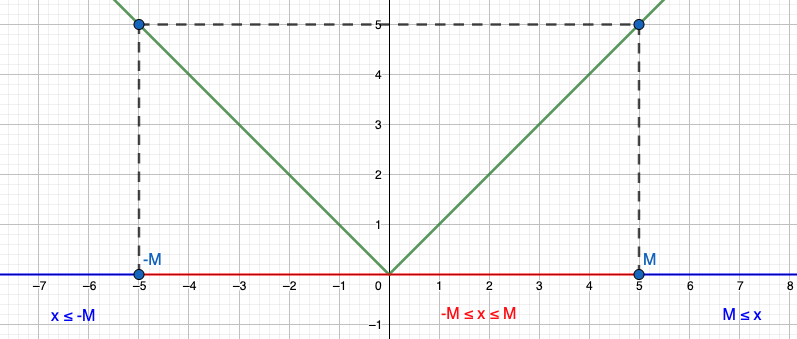
\includegraphics[width=10cm]{es-proprieta-valore-assoluto.png}
    \caption{Spiegazione proprietà 7 e 8}
    \label{fig:prop-6-7}
\end{figure}

\subsection{Disuguaglianza triangolare}
\begin{definition}[Disuguaglianza triangolare]
    Dati due valore $a$ e $b$ tali che $a, b \in \mathbb{R}$ risulta che:
    \begin{equation}
        (1)\:\:\:|a + b| \leq |a| + |b| \hspace{.7cm} (2)\:\:\:||a| + |b|| \leq |a - b| 
    \end{equation}
\end{definition}
\begin{demostration}
    Dimostrazione proprietà (1):\\
    Dati due valori $a$ e $b$ calcoliamo il valore assoluto, che per la proprietà (6) in tabella \ref{tab:prop-valore-assoluto}  possiamo scrivere nella seguente forma:
    \begin{equation}
            -|a| \leq a \leq |a| \hspace{.6cm} -|b| \leq b \leq |b|
    \end{equation}
    Ora facciamo una somma di disuguaglianze fra le forme riportate sopra:
    \begin{equation}
        - |a| - |b| \leq a + b \leq |a| + |b|
    \end{equation}
    Possiamo vedere la prima parte $-|a| - |b|$ come un -M, la parte $a + b$ come una $x$ e l'ultima parte $|a| + |b|$ come M. Utilizzando a questo punto la proprietà (7) in tabella \ref{tab:prop-valore-assoluto}, $|x| \leq M$ quindi:
    \begin{equation}
        |a + b| \leq |a| + |b|
    \end{equation}
\end{demostration}
\begin{observation}
Perché una disuguaglianza triangolare a 3 numeri, $|a + b + c| \leq |a| + |b| + |c|$, vale?\\ \\
Perché se $|a + b + c|$ lo dividiamo in $|(a + b) + c|$ possiamo applicare la propria triangolare su 2 valori considerando $(a+b)$ il primo e $c$ il secondo questo fa si che $|(a + b) + c| \leq |a + b| + |c|$ andando poi a riapplicare la disuguaglianza triangolare questa volta solo su $|a + b|$ vediamo che:
\begin{equation}
    |a + b + c| = |(a + b) + c| \leq |a + b| + |c| \leq |a| + |b| + |c|
\end{equation}
Da qui possiamo dedurre che la disuguaglianza triangolare vale indipendentemente dal numero di valori:
\begin{equation}
    |a_1, a_2, a_3, ..., a_n| \leq |a_1| + |a_2| + |a_3| + .... + |a_n|
\end{equation}
\end{observation}
\newpage
\section{Continuità}
\begin{definition}[Funzione continua]
    Dato un insieme A ed una funzione $f(x)$ tale che $A \subset \mathbb{R}$, $f: A \longrightarrow \mathbb{R}$, la funzione $f$ si dice \textbf{continua} in $x_0$ se $\forall \: \: \epsilon > 0 \: \: \exists \: \: \delta > 0$ tale che se data una $x \in A$:
    \begin{equation}\label{funzione-continua}
        |x - x_0| < \delta \Longrightarrow |f(x) - f(x_0)| < \epsilon
    \end{equation}
\end{definition}
La condizione scritta sopra [\ref{funzione-continua}] può essere scritta anche tramite due condizioni:
\begin{itemize}
    \item $|x - x_0| < \delta \Longleftrightarrow x_0 - \delta < x < x_0 + \delta$
    \item $|f(x) - f(x_0)| < \epsilon \Longleftrightarrow f(x_0) - \epsilon < f(x) < f(x_0) + \epsilon$
\end{itemize}
\begin{example}
Ora per capire meglio facciamo un esempio di funzione non continua:
\end{example}
Innanzitutto stabiliamo una $f(x)$ e verifichiamo che $f(x)$ in $x_0 = 0$ non è continua.\\ 
\begin{wrapfigure}{r}{8cm}
\vspace{-20pt}
    \centering
    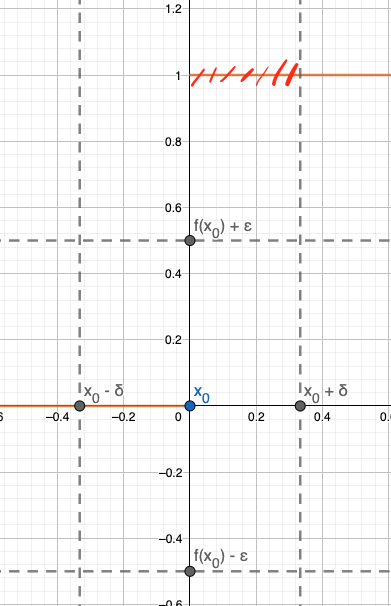
\includegraphics[width=4.8cm, height=5cm]{images/esempio-non-continuita.png}
    \caption{funzione non continua}
    \label{fig:funzione-non-continua}
\end{wrapfigure}

$
  f(x)=\begin{cases}
    0 \: \: se & x \leq 0\\
    1 \: \: se & x > 0
  \end{cases}
$\\ \\ \\
Come prima cosa stabiliamo un $\epsilon = \frac{1}{2}$. Ora, qualunque sia $\delta > 0$ se andiamo a prendere una $x$ tale che $x \in (0, \delta) \Longrightarrow f(x) = 1$ quindi la disuguaglianza $f(x_0) - \epsilon > f(x) < f(x_0) + \epsilon$, che diventerebbe $0 - \frac{1}{2} < f(x) < 0 + \frac{1}{2}$, è falsa. \\ \\
Deduciamo quindi che in $x_0 = 0$ questa funzione non è continua. \\ \\

\begin{definition}
    Dato un insieme A ed una funzione $f(x)$ tale che $A \subset \mathbb{R}$, $f: A \longrightarrow \mathbb{R}$ ed un insieme $B \subset \mathbb{R}$ si dice che $f$ è continua in B e $f$ è continua in ogni punto $x_0 \in B$.
\end{definition}
Se invece si dice semplicemente che $f$ è continua senza specificare il sotto insieme B vuol dire che $f$ è continua in tutti i punti del suo dominio A.
\begin{example}
    Esempio basato sulla funzione vista sopra:\\\\
    $
      f(x)=\begin{cases}
        0 \: \: se & x \leq 0\\
        1 \: \: se & x > 0
      \end{cases}
    $ \hspace{1cm}
    $f$ è continua in $(-\infty, 0) \cup (0, +\infty)$ 
\end{example}

\subsection{Permanenza del segno}
\begin{theorem}[Permanenza del segno]\label{permanenza-segno}
    Dato un insieme A ed una funzione $f$ tale che $A \subset \mathbb{R}$, $f: A \longrightarrow \mathbb{R}$, $x_0 \in A$. Se $f$ è continua in $x_0$ e $f(x_0) > 0$ allora $\exists \: \: \delta > 0$ t.c. se $x \in A$ è $|x - x_0| < \delta \longrightarrow f(x) > 0$. Analogo risultato se $f(x_0) < 0$.
    \begin{demostration}
    Sappiamo che $f(x_0) > 0$. Ora scegliamo un $\epsilon = \frac{f(x_0)}{2}$ ed utilizziamolo nella definizione di continuità:
    \begin{equation}
        \exists \: \: \delta > 0 \: \: | \: \: x \in A, |x - x_0| < \delta \Longleftarrow |f(x) - f(x_0)| < \epsilon
    \end{equation}
    Ciò che risulta dalle condizioni poste dalla continuità è che:
    \begin{equation}
        f(x_0) - \epsilon < f(x) < f(x_0) + \epsilon
    \end{equation}
    Se prendiamo la prima parte $f(x_0) - \epsilon < f(x)$ e facciamo le dovute sostituzioni risulta che:
    \begin{equation}
        f(x_0) - \frac{f(x_0)}{2} < f(x)
    \end{equation}
    Visto che $f(x_0) - \frac{f(x_0)}{2}$ è sempre maggiore di 0 risulta anche che $f(x)$ è maggiore di 0. $\blacksquare$
    \end{demostration}
    \begin{corollaries}\label{collorartio-permanenza-segno}
        Se $f$ è continua in $x_0$ $f: A \longrightarrow \mathbb{R}$, $x_0 \in A$ e $f(x_0) > M$ con $M \in \mathbb{R}$, $x \in A$, $|x - x_0| < \delta \Longrightarrow f(x) > M$. (Vale anche con $f(x_0) < M \Longrightarrow f(x) < M$)
    \end{corollaries}
    \begin{demostration}[Dimostrazione del corollario \ref{collorartio-permanenza-segno}]
        La dimostrazione di questo corollario è immediata e si fa applicando al teorema precedente \ref{permanenza-segno} la funzione $g(x) = f(x) - M$, perché se la funzione $f(x) - M > 0$ è come dire $f(x) > M$. $\blacksquare$
    \end{demostration}
\end{theorem}

\subsection{Continuità con operazioni fra funzioni}
\begin{theorem}
    Prendendo due funzioni $f$ e $g$ continue in un punto $x_0$ allora le funzioni $f + g$, $f * g$ e $|f|$, se inoltre $f(x_0) \neq 0$ allora anche $\frac{1}{f}$ è continua.
    \begin{corollaries}
        Prendendo due funzioni $f$ e $g$ continue in un punto $x_0$ allora $\frac{f}{g}$ è continua se $g(x_0) \neq 0$
    \end{corollaries}
\end{theorem}

\subsection{Funzioni invertibili e continuità}
\begin{proposition}\label{proposizione-funzione-inversa}
    Prendendo due insiemi I (I deve essere un intervallo) e B tale che $I \subset \mathbb{R}$ e $B \subset \mathbb{R}$ ed una funzione $f: I \longrightarrow B$, se $f$ è continua in $I$ ed è invertibile allora $f^{-1}$ è continua in B.
\end{proposition}
\begin{observation}
    Possiamo osservare che ipotesi della proposizione \ref{proposizione-funzione-inversa} dice che il domino sia un intervallo, questo non può essere omesso. 
\end{observation}
\begin{example}
    Verifichiamo questa osservazione con un' esempio:\\
    Prendiamo una funzione $f(x)$ definita in $f: (-\infty, 1] \cup (2, +\infty) \longrightarrow \mathbb{R}$ \: \: \: $f(x) = 
    \begin{cases}
        x \: \: se & x \leq 1 \\
        x - 1 \: \: se & x > 1
    \end{cases}
    $\\
    Qui di seguito le rappresentazioni della funzione $f(x)$ e della sua inversa $f(x)^{-1}$
\end{example}
\begin{figure}[h!]
    \vspace{10pt}
    \begin{subfigure}{.5\textwidth}
        \centering
        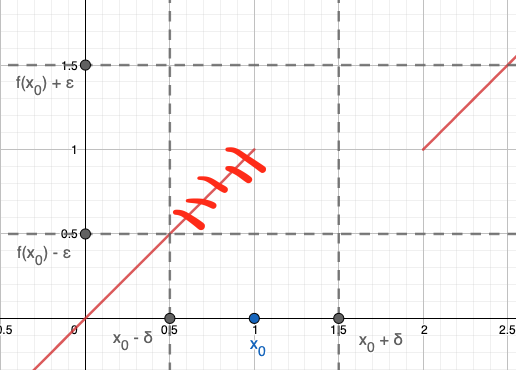
\includegraphics[width=5.5cm]{images/esempio1-osservazione-prop1.png}
        \caption{Osservazione proposizione \ref{proposizione-funzione-inversa}, funzione $f(x)$}
        \label{fig:es1-prop1}
    \end{subfigure}
    \begin{subfigure}{.5\textwidth}
        \centering
        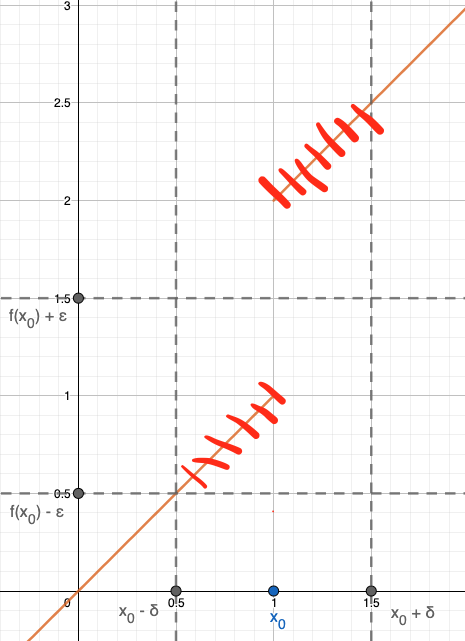
\includegraphics[width=4.2cm, height=5.2cm]{images/esempio2-osservzione-prop1.png}
        \caption{Osservazione proposizione \ref{proposizione-funzione-inversa}, funzione $f(x)^{-1}$}
        \label{fig:es2-prop1}
    \end{subfigure}
\end{figure}
\begin{itemize}
    \item \textbf{Domanda 1°:} $f$ è continua in $x_0 = 1$?\\
    La risposta a questa prima domanda è SI, essendo che noi andiamo a considerare solo i punti all'interno del dominio, quindi la parte compresa fra 1 e 2, dove la funzione presenta una discontinuità, non si considera.
    \item \textbf{Domanda 2°:} $f$ è continua in $x_0 = 2$?\\
La risposta in questo caso è che non ha senso considerare il punto $x_0 = 2$ visto che 2 non fa parte del dominio.
\end{itemize}
Quindi $f$ è continua in tutto il suo dominio. Essendo $f$ continua in tutto il suo dominio allora teoricamente $f^{-1}$ è una funzione invertibile. \\ \\
Possiamo però vedere che la funzione $f^{-1}$, figura [\ref{fig:es2-prop1}] non è continua in $x_0 = 1$ perché essendo la funzione inversa $f^{-1}$ è definita come $f^{-1}: \mathbb{R} \longrightarrow (-\infty, 1] \cup (2, +\infty)$, quindi dobbiamo considerare come dominio tutto $\mathbb{R}$, così facendo ci sono dei punti, in particolare con $x > 0$ che non rientrano nell'intervallo fra $f(x_0) - \epsilon$ e $f(x_0) + \epsilon$ . \\ \\
In conclusione da questo esempio deduciamo che, se $f$ non è definita in un intervallo potrebbe succedere che $f^{-1}$ non è continua anche se $f$ è continua.

\subsection{Continuità delle funzioni elementari}
$f(x) = x$ è una funzione continua. Da questa considerazione segue che tutte le funzioni con polinomi sono continue.
\begin{note}
    Ricorda che anche le funzioni costanti sono sempre continue
\end{note}
Definiamo in maniera generica così una funzione formata da polinomi continua:
\begin{equation}
    P(x) = a_n * x^n + a_{n-1} * x^{n-1} + .... + a_1 * x + a_0 \: \: con \: \: a_0, a_1, ..., a_n \in \mathbb{R}
\end{equation}
Quindi: $x^2 = x * x$ è continua \hspace{.5cm} $x^3 = x^2 * x$ è continua \hspace{.5cm} $x^n$ è continua $\: \: \forall x \in \mathbb{N}$ \\ \\
Le funzioni razionali sono continue nel loro insieme di definizione. Le funzioni razionali sono uguali a quoziente di polinomi:
$f(x) = \frac{p(x)}{q(x)}$ con $p,q$ polinomi, la funzione $f(x)$ è definita se $q(x) \neq 0$.\\ \\
Assumendo che $e^x$, $\sin{x}$, $\cos{x}$ sono funzioni continue quindi anche $\log{x}$, $\arcsin{x}$, $\arccos{x}$, $\tan{x}$, $\arctan{x}$ sono continue.

\subsection{Continuità fra composizione di funzioni}
\begin{theorem}
    Date due funzioni $f: A \longrightarrow \mathbb{R}$ e $g: B \longrightarrow \mathbb{R}$, ed un $x_0 \in A$, $y_0 = f(x_0) \in B$.
    Se $f$ è continua in $x_0$ e $g$ è continua in $y_0$ allora $g \bullet f$ è continua in $x_0$.
\end{theorem}
\begin{example}
    Facciamo un esempio usando la funzione $e^{\cos{x}}$.\\
    $e^{\cos{x}}$ è una funzione continua perché è la composizione di $f(x) = \cos{x}$, funzione continua, e $g(x) = e^y$, pure essa funzione continua.
\end{example}
\begin{observation}
    Data una $f: [a, b] \longrightarrow \mathbb{R}$ continua in $[a, b]$ allora sup($f(x)$) con $x \in (a, b)$ = sup($f(x)$) con $x \in [a, b]$. E ugualmente inf($f(x)$) con $x \in (a, b)$ = inf($f(x)$) con $x \in [a, b]$.
\end{observation}
\begin{example}
    $f(x) = x^2$ con $f: [0,1] \longrightarrow \mathbb{R}$\\
    sup($f(x)$) = $f(1) = 1$ con $x \in [0, 1]$ \hspace{.5cm} sup($f(x)$) = $f(1) = 1$ con $x \in (0, 1)$ \footnote{Ricorda che sup(imm($f(x)$)) = sup(0, 1) = 1}
\end{example}

\subsection{Teorema degli zeri}
\begin{theorem}[Teorema degli zeri]
    Data una $f: [a, b] \longrightarrow \mathbb{R}$ continua. Se $f(a) \cdot f(b) < 0$ allora $\exists c \in (a, b)$ tale che $f(c) = 0$
\end{theorem}
Questo teorema dice che prendendo una funzione, che deve essere obbligatoriamente continua, se i valori di $f(x)$ nei due estremi moltiplicati fra di loro risultano minori di 0 la funzione passa per 0 in un ponto $c$ e questo accade perché se il prodotto fra i due estremi torni inferiore a 0 vuol dire che hanno segno discorde.\\
\begin{example}
    Facciamo un esempio di un caso in cui la funzione NON è continua:
\end{example}
\begin{wrapfigure}{r}{5cm}
    \vspace{-10pt}
    \centering
    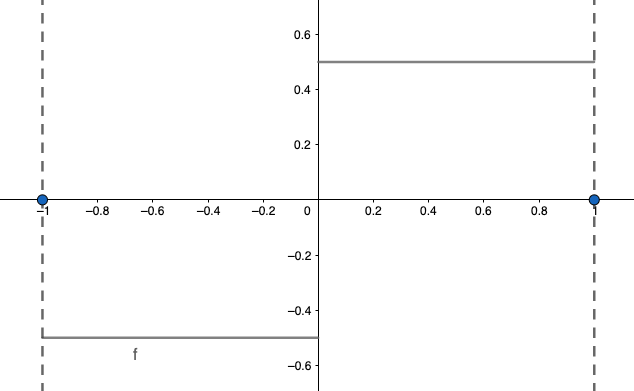
\includegraphics[width=4.5cm, height=2cm]{images/esempio-teorema-zeri.png}
    \caption{$f(x) = [x] + \frac{1}{2}$}
    \label{fig:esempio-teorema-zeri}
\end{wrapfigure}
Prendiamo $f(x) = [x] + \frac{1}{2}$ \: $f: [1, -1] \longrightarrow \mathbb{R}$\\ \\
Se ora prendiamo la f(x) nei due estremi e facciamo il prodotto torna che: \\
$f(1) \cdot f(-1) < 0$ ma $\nexists x \in [-1.1]$ t.c. $f(x) = 0$ come possiamo vedere nell'immagine \ref{fig:esempio-teorema-zeri}.\\ \\

\subsection{Teorema valori intermedi}
\begin{theorem}[Teorema dei valori intermedi]
    Prendendo un intervallo $I \subset R$, ed una funzione $f: I \longrightarrow \mathbb{R}$ continua, allora $f(I)$ è un intervallo.
\end{theorem}
Questo teorema dice che se il nostro dominio è un intervallo e la $f$ è continua all'ora anche il codominio o immagine di $f$ sarà un intervallo.
\begin{corollaries}
    Prendendo sempre un $I \subset R$, una funzione $f: I \longrightarrow \mathbb{R}$ continua, se $f$ assume $y_1$ e $y_2$ allora assume anche tutti i valori compresi fra $y_1$ e $y_2$.
\end{corollaries}

\subsection{Teorema di Weirstrass}
\begin{theorem}[Teorema di Weirstrass]
    Data una funzione $f: [a, b] \longrightarrow \mathbb{R}$ continua. Allora f ha massimo e minimo.
\end{theorem}
\begin{note}
    Notare che $a,b \in \mathbb{R}$ e non in $\overline{\mathbb{R}}$ perché $a, b \neq \pm \infty$ e gli estremi devono essere compresi.
\end{note}
\begin{example}
    Facciamo ora un esempio per confermare come il teorema di Weirstrass possa valore solo con un intervallo chiuso:\\
    Dato $f(x) = \frac{1}{x}$ con $f(x): (0, 1] \longrightarrow \mathbb{R}$ \\ \\in questo caso $f$ ha come dominio un intervallo non chiuso a sinistra\\
    $f$ è continua ma non ha max perché sup($f$) = $+\infty$
\end{example}
\begin{example}
    Facciamo ora un esempio per confermare come il teorema di Weirstrass possa valore solo con un intervallo limitato:\\
    Dato $f(x) = \arctan{x}$ con $f(x): \mathbb{R} \longrightarrow \mathbb{R}$ \\ \\in questo caso $f$ è una funzione continua definita come $-\frac{\pi}{1} < f(x) < \frac{\pi}{2}$\\
    Possiamo notare però che f non toccherà mai ne $-\frac{\pi}{2}$ ne $\frac{\pi}{2}$ e quindi non ha ne massimo ne minimo.
\end{example}
\newpage
\section{Limiti}
\subsection{Intorni}
\begin{definition}[Intorno]
    Dato $x_0 \in \mathbb{R}$ si dice \textbf{intorno} di $x_0$ un insieme del tipo $(x_0 - \epsilon, x_0 + \epsilon)$ dove $\epsilon \in \mathbb{R}$, e $\epsilon > 0$. Inoltre $\epsilon$ si dice raggio dell'intorno
\end{definition}
\begin{itemize}
    \item Un insieme del tipo $[x_0, x_0 + \epsilon]$ si dice \textbf{intorno destro} di $x_0$.
    \item Un insieme del tipo $[x_0 - \epsilon, x_0]$ si dice \textbf{intorno sinistro} di $x_0$.
\end{itemize}
\begin{definition}
    Se $x_0 = +\infty$ un intorno di $x_0$ è un insieme del tipo $(a, +\infty)$\footnote{$(a, +\infty)$ è una semiretta} dove $a \in \mathbb{R}$
\end{definition}
\begin{definition}[Punto di accumulazione]
    Dato $A \subset \mathbb{R}$ e $x_0 \in \overline{R}$ $x_0$ si dice \textbf{punto di accumulazione} per A se $\forall \: U$ intorno di $x_0$ risulta che $U \cap A \setminus \{x_0\} \neq 0$
\end{definition}
Questa definizione vuol dice che "vicino" a $x_0$ ci sono altri punti di A oltre a $x_0$ ($x_0$ potrebbe anche non appartenere ad A).
\begin{example}
    Prendiamo un intervallo A = (2, 3).
\end{example}
Se prendiamo un punto $x_0$ che appartiene a A, quindi $x_0 \in (a,b)$, allora ogni intorno di $x_0$ interseca A in infiniti punti, quindi $x_0$ è un punto di accumulazione di A.\\
\begin{definition}[Intorno bucato]
    Se invece non andiamo a considerare $x_0$ nel suo intorno si dice \textbf{Intorno bucato} e si scrive come $\{x_0 - \epsilon, x_0 + \epsilon\} \setminus \{x_0\}$
\end{definition}
\begin{wrapfigure}{r}{8cm}
    \centering
    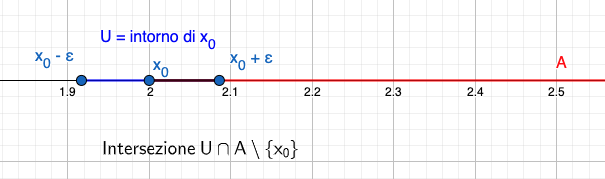
\includegraphics[width=7cm]{images/esempio-intorno-su-estremi.png}
    \caption{Punto di acc $x_0 = 2$ dell'intervallo A}
\end{wrapfigure}

Ora andiamo a dimostrare come tutti i punti [2,3] $\in$ acc(A).
Se poniamo per esempio $x_0 = 2$. Se andiamo a prendere un intorno di $x_0$ nonostante il $\epsilon$ possa essere piccolissimo esisteranno sempre infiniti punti nell'intersezione fra $U$ intorno e $A$ ($U \cap A \setminus \{x_0\}$) perché qualsiasi sia l'epsilon $2 + \epsilon$ rientrerà sempre in A.\\
Questo anche con $x_0 = 3$. 
\begin{note}
Nota che oltre a tutto [2,3] $\in$ A non esisto altri punti di accumulazione di un intervallo A.
\end{note}

\begin{definition}[Punto isolato]
    Dato un insieme A, $x_0 \in A$ si dice \textbf{punto isolato} di A se esiste un $U$ intorno di $x_0$ tale che $U \cap A = \{x_0\}$
\end{definition}
\begin{example}
    Facciamo un osservazione con un intorno spezzato per vedere un caso di punto isolato.
\end{example}
\begin{wrapfigure}{l}{8cm}
    \centering
    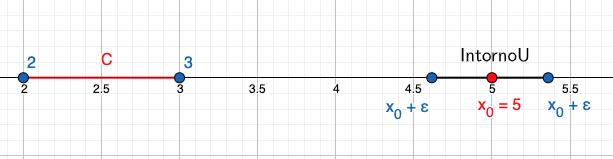
\includegraphics[width=7.3cm, height=2.7cm]{images/esempio-intorno-sepezzato.png}
    \caption{Punto di acc $x_0 = 5$ dell'intervallo C}
\end{wrapfigure}

Se prendiamo un punto C = $(2,3) \cup \{5\}$ non possiamo dire che tutti i punti dell'intervallo C siano punti di accumulazione perché se prendiamo $x_0 = 5$ possono esistere dei casi in cui il suo intorno non interseca C (con U intorno di $x_0 = 5$, $U \cap C \setminus {5} = \O$).\\
Diciamo quindi che in questo caso acc(c) = [2,3]\\\\
\begin{example}
    Esempio in cui verifichiamo come, dato un insieme D = $(3, +\infty)$, sia $+\infty \in$ acc(D).\\
    Come prima cosa prendiamo un $U$ intorno di $x_0 = +\infty$. Quindi $U = (a, +\infty)$.\\
    Definiamo ora il punto maggiore fra 3 ed $a$, $b =$ max($3,a$), questo punto sarà l'estremo sinistro dei punti di accumulazione.
    Facciamo ora l'intersezione:
    \begin{center}
        $U \cap D \setminus \{x_0\} = (2, +\infty) \cap (a, +\infty) \setminus {+\infty} = (b, +\infty) \neq \O$.
    \end{center}
    Vediamo dunque che $+\infty$ è un punto i accumulazione di D, quindi acc(D) = $[b, +\infty]$.
\end{example}
\newpage
\begin{example}
    Esempio prendendo come insieme $E = \mathbb{N}$.
\end{example}
\begin{wrapfigure}{r}{7cm}
    \vspace{-15pt}
    \centering
    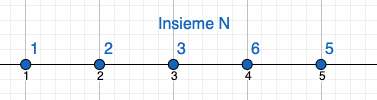
\includegraphics[width=6.2cm]{images/insieme-N.png}
    \caption{Insieme $\mathbb{N}$}
    \label{fig:insieme-N}
\end{wrapfigure}

Se osserviamo l'immagine \ref{fig:insieme-N} vediamo chiaramente come tutti gli elemento di $\mathbb{N}$ sia punti isolare e quindi non siano punti di accumulazione. Ma, per l'esempio visto sopra, $+\infty$ è l'unico punto di accumulazione di $\mathbb{R}$. Acc($\mathbb{N}$) = $+\infty$. \\
\begin{note}
    Allo stesso modo prendendo in considerazione l'insieme $\mathbb{Z}$ i suoi punti di accumulazione sono acc($\mathbb{Z}$) = $\{-\infty, +\infty\}$
\end{note}
\begin{definition}
    Dato un insieme $A \subset \mathbb{R}$, ed un $x_0 \in A$, si dice $x_0$ punto interno ad A se esiste un $U$ intorno di $x_0$ tale che $U \subset A$. L'insieme dei punti interni si indica con int(A).
\end{definition}
\begin{example}
    Dato un A = [3, 5] i punti intesi sono (3,5) e non [3,5] perché se prendiamo $x_0 = 3$ o $x_0 = 5$ essendo che l'intorno di $x_0$ è [$x_0 - \epsilon$, $x_0 + \epsilon$] rimarrà sempre una parte fuori, in particolare quella di sinistra per $x_0 = 3$, e quella di destra per $x_0 = 5$.
\end{example}

\subsubsection{Minimi e massimi locali}
\begin{definition}[Minimi e massimi locali e locali stretti]
    Dato un insieme $A \subset \mathbb{R}$, una funzione $f: A \longrightarrow \mathbb{R}$ ed un punto $x_0 \in A$ si dice che $x_0$ è:
    \begin{itemize}
        \item \textbf{Minimo locale} (o relativo) se esiste un $U$ intorno di $x_0$ tale che $f(x) \geq f(x_0) \: \forall \: x \in U \cap A$
        \item \textbf{Minimo locale stretto} se esiste un $U$ intorno di $x_0$ tale che $f(x) > f(x_0) \: \forall \: x \in U \cap A \setminus \{x_0\}$
        \item \textbf{Massimo locale} (o relativo) se esiste un $U$ intorno di $x_0$ tale che $f(x) \leq f(x_0) \: \forall \: x \in U \cap A$
        \item \textbf{Massimo locale stretto} se esiste un $U$ intorno di $x_0$ tale che $f(x) < f(x_0) \: \forall \: x \in U \cap A \setminus \{x_0\}$
    \end{itemize}
\end{definition}
Questa definizione vuol dire che se andiamo a prendere un intorno di $x_0$, il punto $x_0$ può essere definito minimo o massimo di quel determinato intorno se è il punto più "in basso" o più "in alto" rispetto a tutti gli altri punti dell'intorno.
\begin{figure}[h!]
    \begin{subfigure}{.5\textwidth}
        \centering
        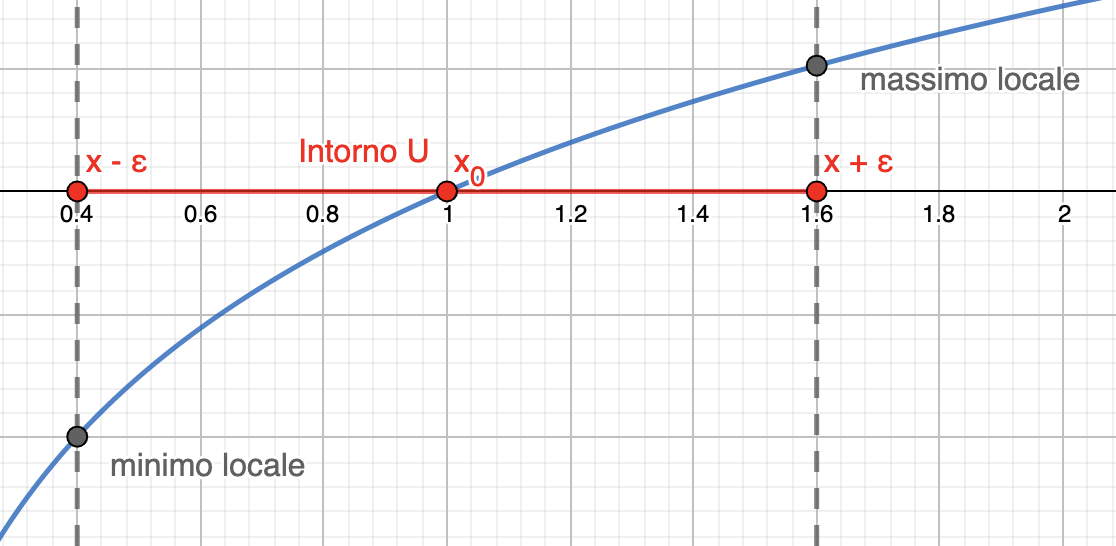
\includegraphics[width=7.7cm]{images/min-max-locale.png}
        \caption{Minimo e massimo locale}
        \label{fig:min-max-locale}
    \end{subfigure}
    \begin{subfigure}{.5\textwidth}
        \centering
        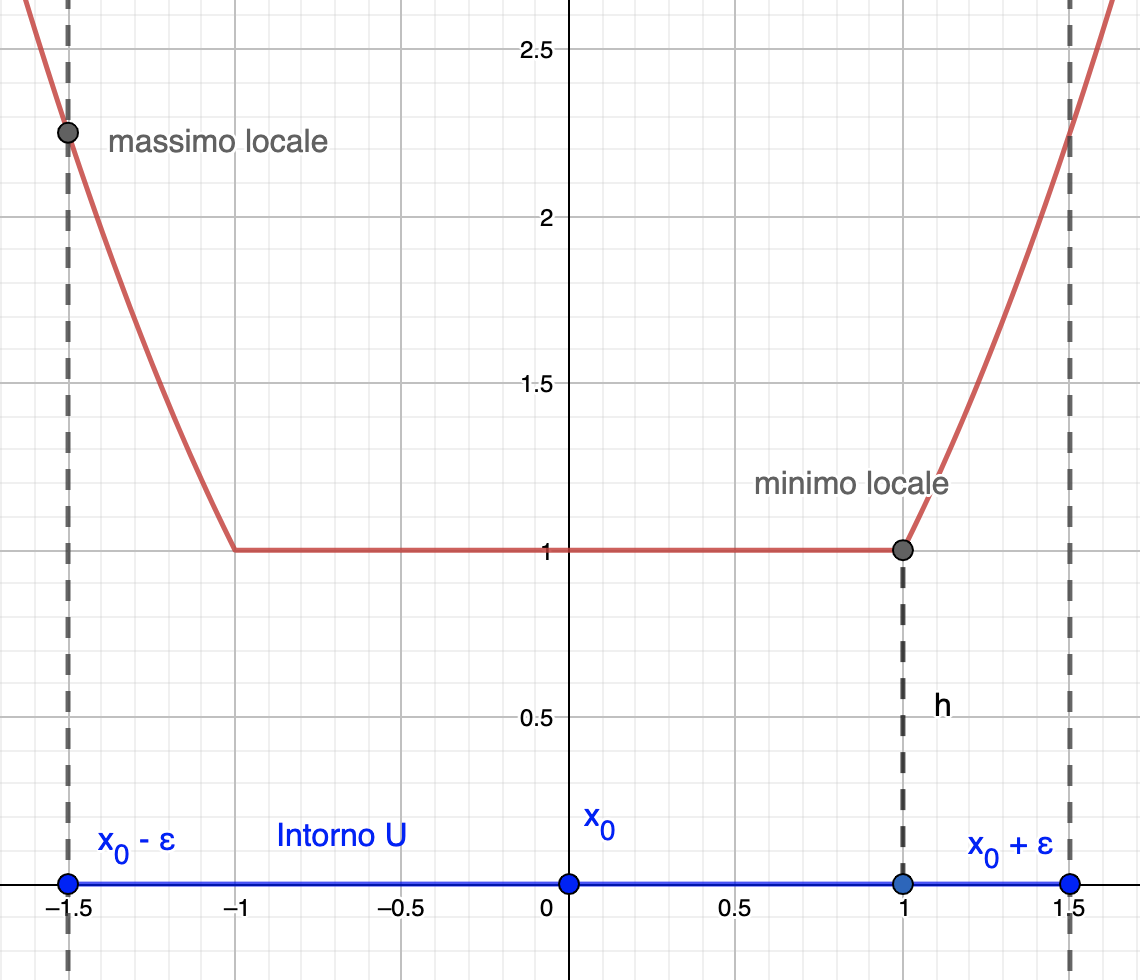
\includegraphics[width=5.5cm]{images/min-max-locale-stretto.png}
        \caption{Minimo e massimo locale stretto}
        \label{fig:min-max-locale-stretto}
    \end{subfigure}
\end{figure}

Come si può vedere dalle immagini [\ref{fig:min-max-locale}] [\ref{fig:min-max-locale-stretto}] noi andiamo a considerare solo i punti all'interno dell'intorno di $x_0$, infatti esisterebbero altri punti esterni a $U$ intorno maggiori o minori, ma non li consideriamo.
\begin{note}
    Nota che se $x_0$ è punto di minimo allora è anche punto di minimo locale, qualsiasi sia l'intorno che prendiamo in considerazione.
\end{note}

\subsection{I limiti}
\begin{definition}[Limite]
    Dato un $A \subset \mathbb{R}$, una $f: A \longrightarrow \mathbb{R}$, ed un $x_0$ punto di accumulazione per A, si dice che $l \in \overline{\mathbb{R}}$ è il limite per $x$ che tende a $x_0$ di $f(x)$ se $\forall$ V intorno di $l$, $\exists \: U$ intorno di $x_0$ t.c. $x \in U \cap A \setminus \{x_0\} \Longrightarrow f(x) \in V$
\end{definition}
Questa definizione dice che un valore $l$ per essere definito come limite di una funzione con $x$ che tende a $x_0$ bisogna che per qualsiasi intorno che andiamo a prendere di $l$ deve esistere una intorno di $x_0$ chiamato U tale che, se una $x$ appartiene ad U allora la $f(x)$ apparterrà all'intorno di $l$. \\
Se ci rifacciamo alle definizioni di intorno vediamo che $x \in U \cap A \setminus \{x_0\}$ vuol dire che $|x-x_0| < \delta$ e che $f(x) \in V $ vuol dire che $l - \epsilon < f(x_0) < l + \epsilon$.\\
Questa definizione può essere scritta in altre parole dicendo che:
\begin{center}
    $\lim\limits_{x\to x_0}f(x) = l$\footnote{La notazione $\lim\limits_{x\to x_0}f(x)$ è quella con cui andiamo a scrivere i limiti e vuol dire limite di $f(x)$ con $x$ che tende a $x_0$ è uguale a $l$ valore del limite} $ \Longleftrightarrow \forall \epsilon > 0 \: \: \exists \delta > 0 $ tale che $x \in A, |x - x_0| < \delta \land x \neq x_0 \Longrightarrow |f(x) - f(x_0)| < \epsilon$
\end{center}
\begin{example}
Alcuni esempi di limiti:
\begin{itemize}
    \item $\lim\limits_{x\to x_0}f(x) = \pm \infty$ \hspace{.5cm} $V = (a, \pm \infty)$ \hspace{.5cm} $f(x) \in V$ se e solo se $f(x) > a$\\
    Il risultato di questo limite è $\pm \infty$ se $\forall a \in \mathbb{R} \: \exists \: \delta > 0$ t.c. $|x-x_0|<\delta, x \in A, x\neq x_0 \Longrightarrow f(x) > a$
    \item $\lim\limits_{x\to \pm \infty}f(x) = l$ \hspace{.5cm} se $l \in \mathbb{R}$ se e solo se $x \to \infty$\\
    Il risultato del limite è un valore appartenete a $\mathbb{R}$ se $\forall \epsilon > a \: \exists a \in \mathbb{R}$ t.c. $x > a \Longrightarrow |f(x) - l| < \epsilon$
    \item $\lim\limits_{x\to \pm \infty}f(x) = \pm \infty$ \:
    se e solo se $\forall a \in \mathbb{R} \exists b \in \mathbb{R}$ t.c. $x > b \Longrightarrow f(x) > a$
\end{itemize}
\end{example}
\begin{theorem}[Unicità dei limiti]
Se esiste un limite di $f$ con $x \to x_0$, questo limite è unico.
\end{theorem}

\subsection{Continuità con i limiti}
Rivediamo le definizioni di limiti (con il limite che sia un numero finito)  e continuità accanto:
\begin{enumerate}
    \item $\lim\limits_{x\to x_0}f(x) = l$ con $x_0 \in A$, $l \in \mathbb{R}$ è vera se e solo se $\forall\epsilon > 0 \: \: \exists \delta >0$ t.c. $x \in A, x \neq x_0$ è $|x - x_0| < \delta \Longrightarrow |f(x) - l| < \epsilon$
    \item $f$ è continua in $x_0$ se e solo se $\forall \epsilon > 0 \: \: \exists \delta > 0$ t.c. $|x - x_0| < \delta$ con $x \in A \Longrightarrow |f(x) - f(x_0)| < \epsilon$
\end{enumerate}
Notiamo subito che fra la definizione (1) e la (2) c'è come unica differenza che nella prima c'è $l$ mentre nella seconda c'è $f(x)$. Possiamo dunque trarre una serie di osservazioni.
\begin{observation}
Data una funzione $f(x)$ essa è continua in $x_0 \Longrightarrow \lim\limits_{x\to x_0}f(x) = l$
\end{observation}
\begin{observation}
Una funzione è sempre continua nei punti isolati.
\end{observation}
\begin{observation}
Nella definizione di limite non serve che $x_0$ sia nel dominio di una funzione, basta che sia un punto di accumulazione per il dominio.
\end{observation}
\begin{example}
Esempio di continuità con i limiti:
\end{example}
\begin{wrapfigure}{r}{6cm}
    \vspace{-50pt}
    \centering
    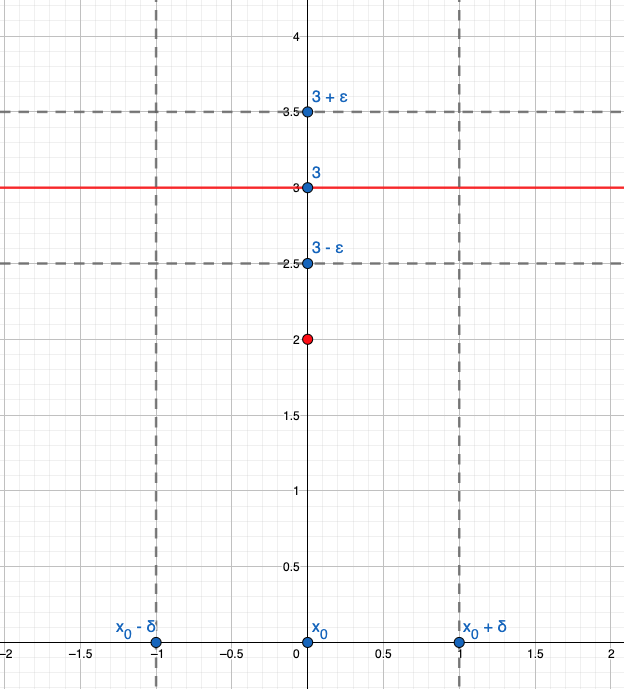
\includegraphics[width=5cm, height=4.7cm]{images/es-continuita-limiti.png}
    \caption{$\lim\limits_{x\to 0}f(x) = 3$}
\end{wrapfigure}

$f(x) = 
    \begin{cases}
        3 \: \: se & x \neq 0 \\
        2 \: \: se & x = 0
    \end{cases}
    $\\ \\
$\lim\limits_{x\to 0}f(x) = 3$, senza considerare f in $x = 0$.\\
Secondo la definizione di continuità di una funzione vista sopra (dove andiamo a guardare il valore del limite in $x_0$):
\begin{center}
    $|x - x_0| < \delta$, $x \in A$, $x \neq x_0$ allora $|f(x) - l| < \epsilon$.
\end{center}
Se andiamo però a vedere $\lim\limits_{x\to 0}f(x) = 3$ mentre $f(0) = 2$ e ovviamente $2 \neq 3$ quindi f non è continua in $x_0$.



\subsection{Limite destro e sinistro}
\begin{definition}[Limite destro e sinistro]
    Se dato un $A \subset \mathbb{R}$, un $x_0 \in Acc(A)$, un $x_0 \in \mathbb{R}$ ($x_0$ deve essere un numero finito), ed  $f: A \to \mathbb{R}$, allora si dice che $l \in \overline{\mathbb{R}}$ è il limite di $f(x)$ per x che tende a $x_0$ da \textbf{destra} (si scrive come $\lim\limits_{x\to x_0^+}f(x) = l$) se:
    \begin{center}
        $\forall \: V$ intorno di $l \: \exists \: \delta > 0$ t.c. $x_0 < x < x_0 + \delta$, $x \in A \Longrightarrow f(x) \in V$
    \end{center}
    Si dice limite \textbf{sinistro} (si scrive come $\lim\limits_{x\to x_0^-}f(x) = l$) se:
    \begin{center}
        $\forall \: V$ intorno di $l \: \exists \: \delta > 0$ t.c. $x_0 - \delta < x < x_0$, $x \in A \Longrightarrow f(x) \in V$
    \end{center}
\end{definition}
\begin{example}
Se prendiamo una $f: (-\infty, 0) \cup (0, +\infty) \to \mathbb{R}$, 
$f(x) = 
    \begin{cases}
        -1 \: \: se & x < 0 \\
        1 \: \: se & x > 0
    \end{cases}
    $ \\ 
    Il $\lim\limits_{x \to 0^+} f(x) = 1$ mentre $\lim\limits_{x \to 0^-} f(x) = -1$. Ciò perché andiamo nel caso del limite destro a guardare il valore "alla destra" di 0 e nel limite sinistro il valore "alla sinistra".
\end{example}
\begin{observation}
$\lim\limits_{x \to x_0^+} = l$ se e solo se $\lim\limits_{x \to x_0^+} = l_1$, $\lim\limits_{x \to x_0^-} = l_2$ e $l_1 = l_2$. Cioè per far in modo che il limite di una funzione che tende ad un valore $x_0$ sia unico bisogna che il limite destre e quello sinistro siano uguali. Nell'esempio precedente infatti possiamo notare che non esiste un unico limite perché i valori del destro e del sinistro sono diversi.
\end{observation}

\subsection{Limite da sopra e da sotto}
Dato un $A \subset \mathbb{R}$, una $f: A \to \mathbb{R}$, ed un $x_0 \in Acc(A)$
\begin{definition}
 Si dice che $\lim\limits_{x \to x_0}f(x) = l^+$ (con $l \in \mathbb{R}$) se $\lim\limits_{x\to x_0}f(x) = l$ ed esiste un $U$ intorno di $x_0$ t.c. $x \in U \cap A \setminus \{x_0\} \Longrightarrow f(x) > l$
\end{definition}
\begin{definition}
 Mentre analogamente si dice che $\lim\limits_{x \to x_0}f(x) = l^-$ (con $l \in \mathbb{R}$) se $\lim\limits_{x\to x_0}f(x) = l$ ed esiste un $U$ intorno di $x_0$ t.c. $x \in U \cap A \setminus \{x_0\} \Longrightarrow f(x) < l$
\end{definition}
Queste due definizione vogliono dire che la funzione può tendere ad un valore "da sopra" nel caso del + e "da sotto" nel caso del -.
\begin{figure}[h!]
    \begin{subfigure}{.5\textwidth}
        \centering
        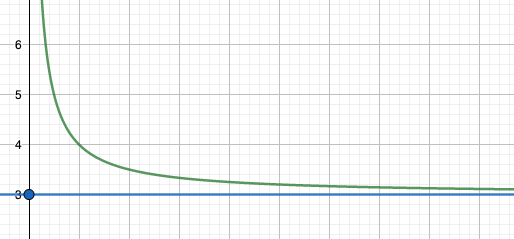
\includegraphics[width=5.5cm]{images/limite-tende-sopra.png}
        \caption{Limite che tende da sopra}
    \end{subfigure}
    \begin{subfigure}{.5\textwidth}
        \centering
        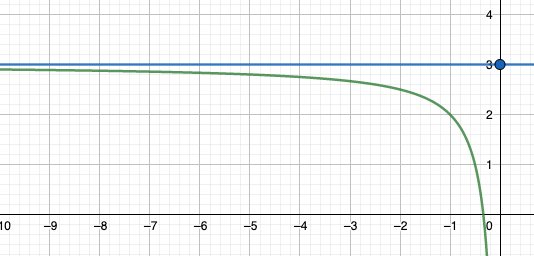
\includegraphics[width=5.5cm]{images/lim-tende-sotto.png}
        \caption{Limite che tende sa sotto}
    \end{subfigure}
\end{figure}
\begin{example}
Un esempio è con $f(x) = \frac{1}{x}$ dove $\lim\limits_{x\to x_0}f(x) = 0^+$
\end{example}

\subsection{Permanenza del segno}
\begin{theorem}[Permanenza del segno]
Dato un $A \subset \mathbb{R}$, un $x_0 \in Acc(A)$ se esiste $\lim\limits_{x\to x_0}f(x) = l$, dove $l \in \overline{\mathbb{R}}$ e $l \neq 0$ allora esiste un intorno $U$ di $x_0$ t.c se $x \in U \cap A \setminus \{x_0\}$ allora $f(x)$ ha lo stesso segno di $l$.
\end{theorem}
\begin{example}
$f: (0, +\infty) \to \mathbb{R}$ \hspace{.5cm} $f(x) = \frac{1}{x}$ \hspace{.5cm} $\lim\limits_{x\to 0^+}f(x) = +\infty$ \\
Quindi visto che $+\infty > 0$ se prendiamo un intorno di $x_0$ qualsiasi $f(x)$ con $x$ appartenente all'intersezione fra il dominio e l'intorno (escluso $x_0$) tornerà che $f(x) > 0$. 
\end{example}

\subsection{Non esistenza di un limite}
Ci sono casistiche di funzioni nel quale un limite non esiste, e quindi no può essere calcolato. Per verificare ciò vediamo alcuni esempi.
\begin{example}
$\lim\limits_{x\to x_0} \sin(x)$ Non esiste. Vediamo perché.
\end{example}
\begin{wrapfigure}{l}{8cm}
    \vspace{-10pt}
    \centering
    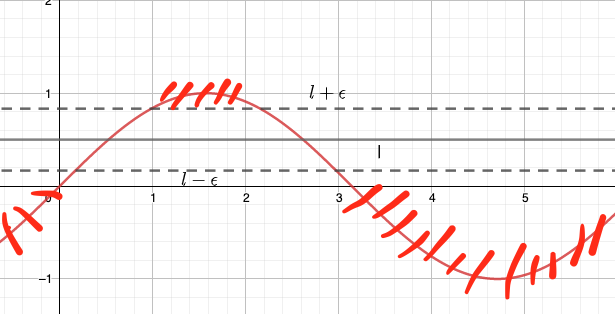
\includegraphics[width=7cm, height=3cm]{images/es-limite-non-esiste.png}
    \caption{Limite che non esiste}
    \label{fig:limite-non-esiste}
\end{wrapfigure}

Supponiamo per assurdo che: \\$\lim\limits_{x\to x_0} \sin(x) = l$\\ \footnote{Ricorda che per la definizione di limite la f(x) deve essere compresa fra $f(x_0) + \epsilon$ e $f(x_0) - \epsilon$ qualsiasi sia il valore di $\epsilon$}Prendiamo ora un valore $\epsilon < \frac{1}{2}$. \\ \\
Se esistesse il limite $l \in \mathbb{R}$ allora dovrebbe esistere $a > 0$ t.c. $x > a \Longrightarrow l - \epsilon < \sin{x} < l + \epsilon$ ma questo assurdo perché vorrebbe dire che $\sin{x}$ oscilla con ampiezza minore di $2\epsilon$ mentre $\sin{x}$ oscilla con ampiezza 2. 
\begin{note}
Nota che nell'immagine \ref{fig:limite-non-esiste} le parti rosse escono dall''intervallo $[l-\epsilon, l+\epsilon]$.
\end{note}

\subsection{Continuità destra e sinistra}
\begin{definition}[Continuità destra e sinistra]\label{continuità-destra-sinistra}
Dato un $A \subset \mathbb{R}$, un $x_0 \in Acc(A)$:
\begin{itemize}
    \item se $\lim\limits_{x \to x_0^+}f(x) = f(x_0)$ allora si dice che $f$ è \textbf{continua a destra} in $x_0$.
    \item se $\lim\limits_{x \to x_0^-}f(x) = f(x_0)$ allora si dice che $f$ è \textbf{continua a sinistra} in $x_0$.
\end{itemize}
\end{definition}

\begin{example}
Data una $
f(x) = \begin{cases}
    1 \: \: se & x \geq 0 \\
    -1 \: \: se & x < 0
\end{cases}$\\
Il $\lim\limits_{0^+}f(x) = 1$ mentre $\lim\limits_{0^-}f(x) = -1$\\
Questo esempio ci dice, come spiegato nella definizione sopra (\ref{continuità-destra-sinistra}), che la funzione è continua a destra nel caso di $0^+$ mentre con $0^-$ la funzione non è continua a sinistra perché il risultato del limite $l \neq f(x_0)$. 
\end{example}
\begin{observation}
    Nel esempio sopra possiamo vedere che la funzione è continua in $x_0^+$ ma non in $x_0^-$. Sin può osservare infatti come una funzione $f$ è continua in un punto $x_0$ se e solo se è continua sia a destra che ha sinistra, perché ciò vorrebbe dire che entrambi i limiti, quello da $x_0^-$ e $x_0^+$, avrebbero uno stesso risultato:
    \begin{center}
        $\lim\limits_{x\to x_0^+}f(x) = l_1$ \:\:\: $\lim\limits_{x\to x_0^-}f(x) = l_2$ \:\:\: $l_1 = l_2 = f(x_0)$
    \end{center}
\end{observation}

\subsection{Teorema di confronto}
\begin{theorem}[Teorema di confronto]
    Dato un $A \subset \mathbb{R}$, un $x_0 \in Acc(x)$, e due funzioni $f,g: A \to \mathbb{R}$. Se esiste un $\lim\limits_{x\to x_0}f(x) = l_1$ e $\lim\limits_{x\to x_0}g(x) = l_2$ e se esiste un $U$ intorno di $x_0$ t.c. $x \in U \cap A \setminus \{x_0\}$ e $f(x) \leq g(x)$ allora $l_1 \leq l_2$.
\end{theorem}
Questo teorema in maniera sintetica dice che se una funzione "sta sotto" l'altra a sua volta anche il limite della prima starà sotto il secondo, detto in altre parole la disuguaglianza passa ai limiti:
\begin{center}
    Se $f(x) \leq g(x)$ allora $\lim\limits_{x\to x_0}f(x) \leq \lim\limits_{x\to x_0}g(x)$
\end{center}

\begin{observation}
    Se però esiste $f(x) < g(x)$ non potrei dire che $\lim\limits_{x\to x_0}f(x) < \lim\limits_{x\to x_0}g(x)$. Perché:
\end{observation}
Se prendiamo come esempio due funzioni una $f(x) = -\frac{1}{x}$ e una $g(x) = \frac{1}{x}$ vediamo che $f(x) < g(x)$ ma se calcoliamo i limiti $\lim\limits_{x\to x_0}f(x) = 0$ e $\lim\limits_{x\to x_0}g(x) = 0$ e quindi i limiti sono uguali. Possiamo dunque dire che le disuguaglianze passano al limite ma diventano sempre deboli:
\begin{center}
        Se $f(x) < g(x)$ allora $\lim\limits_{x\to x_0}f(x) \leq \lim\limits_{x\to x_0}g(x)$
\end{center}

\subsection{Teorema somma e prodotto}
\begin{theorem}[Teorema somma e prodotto]
    Dato un $A \subset \mathbb{R}$, un $x_0 \in Acc(A)$, e due funzioni $f,g: A \to \mathbb{R}$. Supponiamo che esistano i limiti $\lim\limits_{x\to x_0}f(x) = l_1$ e $\lim\limits_{x\to x_0}g(x) = l_2$ con $l_1, l_2 \in \overline{\mathbb{R}}$.
    \begin{itemize}
        \item Se ha senso $l_1 + l_2$ allora esiste $\lim\limits_{x\to x_0}(f + g)(x) = l_1 + l_2$.
        \item Se ha senso $l_1 \cdot l_2$ allora esiste $\lim\limits_{x\to x_0}(f + g)(x) = l_1 \cdot l_2$.
    \end{itemize}
\end{theorem}
\begin{note}
Sono esclusi i casi $l_1 = +\infty$ e $l_2 = -\infty$ (o viceversa) per il prodotto. Sono invece esclusi i casi $l_1 = 0$ e $l_2 = \pm\infty$ (o viceversa) per la somma. Questi casistiche sono dette indeterminate e non possono essere calcolate in maniera diretta.
\end{note}

\subsection{Teorema dei carabinieri}
\begin{theorem}[Teorema dei carabinieri]
    Dato un $A \subset \mathbb{R}$, un $x_0 \in Acc(A)$, e due funzioni $f,g,h: A \to \mathbb{R}$. Se esiste $\lim\limits_{x\to x_0}f(x) = l$ e $\lim\limits_{x\to x_0}h(x) = l$ (i due limiti hanno lo stesso risultato) e se esiste un intorno $U$ di $x_0$ t.c. $x \in A \cup U \setminus \{x_0\}$, se $f(x) \leq g(x) \leq h(x)$ allora esiste $\lim\limits_{x\to x_0}g(x) = l$.
\end{theorem}
Il teorema dei carabinieri dice in maniera sintetica che se due funzioni hanno lo stesso limite ed una è inferiore all'altra se esiste una $g(x)$ in mezzo a queste due funzioni avrà lo stesso limite per uno stesso $x_0$, quindi dall'esistenza dei limiti di $f$ e $h$ (uguali) deduco l'esistenza del limite di $g$
\begin{example}
Facciamo un esempio prendendo $\lim\limits_{x\to +\infty}\frac{2 + \sin{(x)}}{x}$.
Prendendo due funzioni $f(x) = \frac{1}{x}$ e $h(x) = \frac{3}{x}$ sapiamo che $\frac{1}{x} \leq \frac{2 + \sin{(x)}}{x} \leq \frac{3}{x}$. \\
Se poi andiamo a calcolare i limiti per $x \to +\infty$ di $f(x)$ e di $h(x)$ vediamo che $\lim\limits_{x\to +\infty}f(x) = 0$ e $\lim\limits_{x\to +\infty}h(x) = 0$.
Allora per il teorema dei carabinieri $\lim\limits_{x\to +\infty}\frac{2 + \sin{(x)}}{x} = 0$
\end{example}

Alcune conseguenze del teorema dei carabinieri visto sopra:
\begin{proposition}
Dato un $A \subset \mathbb{R}$, un $x_0 \in Acc(A)$, e due funzioni $f,g: A \to \mathbb{R}$:
\begin{itemize}
    \item Se $f$è lim. inferiormente in intorno di $x_0$ e $\lim\limits_{x\to x_0}g(x) = +\infty \Longrightarrow \lim\limits_{x\to x_0}(f + g)(x) = +\infty$.
    \item Se $f$è lim. superiormente in intorno di $x_0$ e $\lim\limits_{x\to x_0}g(x) = -\infty \Longrightarrow \lim\limits_{x\to x_0}(f + g)(x) = -\infty$.
    \item Se $f$è limitata in un intorno di $x_0$ e $\lim\limits_{x\to x_0}g(x) = 0 \Longrightarrow \lim\limits_{x\to x_0}(f \cdot g)(x) = 0$.
\end{itemize}
\end{proposition}

\begin{example}
Prendiamo il $\lim\limits_{x\to +\infty}x + \sin(x)$\\
$\lim\limits_{x\to +\infty}x = +\infty$ \hspace{.5cm} $\lim\limits_{x\to +\infty}\sin(x)$ non esiste.\\
Data l'inesistenza del secondo limite non posso applicare il teorema sul limite della somma ma $\sin(x)$ è limitata inferiormente quindi:
Per il teorema dei carabinieri $x - 1 \leq x + \sin(x) \leq x + 2$, e visto che $\lim\limits_{x\to +\infty}x - 1 = +\infty$ e $\lim\limits_{x\to +\infty}x + 2 = +\infty$ possiamo dire che $\lim\limits_{x\to +\infty}\sin(x) = +\infty$
\end{example}

\subsection{Limitatezza funzione con i limiti}
\begin{theorem}
    Dato un $A \subset \mathbb{R}$, un $x_0 \in Acc(A)$, e $f: A \to \mathbb{R}$. Se esiste $\lim\limits_{x\to x_0}f(x) = l$ e $l \in \mathbb{R}$ (quindi $l$ non è $\pm\infty$) allora $f$ è limitata in un intorno di $x_0$ cioè $\exists \: U$ intorno di $x_0$ e $\exists M \in \mathbb{R}$ con $M > 0$ t.c. $x \in U \cap A \Longrightarrow |f(x)| \leq M$.
\end{theorem}
Questo teorema dice che se prendiamo una funzione che ha un limite per $x\to x_0$ che è un valore diverso da $\pm\infty$ e prendiamo un intorno di $x_0$ esisterà un valore M dove per qualsiasi $x \in U \cap A$ il $|f(x)| \leq M$ che corrisponderebbe a $-M \leq f(x) \leq M$ quindi la funzione sarà limitata nell'intorno selezionato.
\begin{example}
Se prendiamo $f(x) = \frac{1}{x}$ è limitata in un intorno di $+\infty$ perché $\lim\limits_{x\to x_0}f(x) = 0$.
\end{example}

\begin{definition}
Dato un $A \subset \mathbb{R}$, un $x_0 \in Acc(A)$, e $f: A \to \mathbb{R}$ possiamo dire che:
\begin{itemize}
    \item Se $\lim\limits_{x\to x_0}f(x) = 0$ allora si dice che $f$ è \textbf{infinitesima} per $x$ che tende a $x_0$.
    \item Se $\lim\limits_{x\to x_0}f(x) = +\infty$ allora si dice che $f$ è \textbf{diverge positivamente} per $x$ che tende a $x_0$.
    \item Se $\lim\limits_{x\to x_0}f(x) = -\infty$ allora si dice che $f$ è \textbf{diverge negativamente} per $x$ che tende a $x_0$.
    \item Se $\lim\limits_{x\to x_0}f(x) = l$ ed $l \in \mathbb{R}$ ($l$ è finito) allora si dice che $f$ è \textbf{converge} in $l$ per $x$ che tende a $x_0$.
\end{itemize}
\end{definition}

\subsection{Forme indeterminate}
\begin{table}[h!]
    \setlength{\tabcolsep}{7pt}
    \renewcommand{\arraystretch}{1.5}
    \centering
    \begin{tabular}{|c c c|}
        \hline
        $[1]$ $(+\infty) + (-\infty)$ & $[2]$ $(-\infty) + (+\infty)$ & $[3]$ $0 \cdot (\pm \infty)$ \\
        $[4]$ $(\pm \infty)^0$ & $[5]$ $(0^+)^0$ & $[6]$ $(1)^{\pm \infty}$\\ 
        \hline
    \end{tabular}
    \caption{Forme indeterminate}
\end{table}
\begin{demostration}
Dimostriamo come la forma [1] e la [2] siano indeterminate (facciamo un esempio considerandone una, ma sono equivalente).\\
Prendiamo un $f(x) = 2x$ e $g(x) = -x$ e facciamo i limiti di entrambi, ed il limite della somma.\\\\
$\lim\limits_{x\to +\infty}f(x) = +\infty$ e $\lim\limits_{x\to +\infty}g(x) = -\infty$, la somma $\lim\limits_{x\to +\infty}(f + g)(x) = 2x - x = x = +\infty$\\
In questo cosa il limite di $(+\infty) + (-\infty)$ torna $+\infty$.\\ \\
Ora prendiamo invece altre due funzioni $f(x) = \frac{x}{2}$ e $g(x) = -x$ e calcoliamo come prima i limiti di entrambi ed il limite della loro somma.\\\\
$\lim\limits_{x\to +\infty}f(x) = +\infty$ e $\lim\limits_{x\to +\infty}g(x) = -\infty$, la somma $\lim\limits_{x\to +\infty}(f + g)(x) = (\frac{x}{2} - x) = -\frac{x}{2} = -\infty$\\
In questo caso invece il limite di $(+\infty) + (-\infty)$ torna $-\infty$.\\\\
Alla domanda, quale scegliamo? La risposta è nessuna delle due, infatti non potendo avere un risultato fisso diciamo che questa è una forma indeterminata.\\
Nota che questa dimostrazione è valida anche per la forma $0 \cdot (\pm \infty)$.
\end{demostration}
Per le forme [4], [5] e [6] possiamo tramite dei calcoli algebrici spiegarle riconducendoci alle prime 3 forme.\\\\
Possiamo infatti vederle come $f(x)^{g(x)} = e^{\log(f(x)^{g(x)}}) = e^{g(x) \cdot \log(f(x))}$ e quindi possiamo analizzare i casi in cui $\lim\limits_{x\to x_0}g(x) \cdot \lim(f(x))$ è indeterminato:
\begin{enumerate}
    \setcounter{enumi}{3}
    \item Con $g\to 0$ e $f\to +\infty \Longrightarrow \log(f(x)) \to +\infty = 0 \cdot +\infty$ (quindi $(+\infty)^0$ è indeterminata).
    \item Con $g\to 0$ e $f\to +0^+ \Longrightarrow \log(f(x)) \to -\infty = 0 \cdot -\infty$ (quindi $(0^+)^0$ è indeterminata).
    \item Con $g\to \pm\infty$ e $f\to 1 \Longrightarrow \log(f(x)) \to 0 = 0 \cdot \pm\infty$ (quindi $(1)^{\pm\infty}$ è indeterminata).
\end{enumerate}

\subsection{Calcolo dei limiti}
\begin{proposition}
Dato un $A \subset \mathbb{R}$, un $x_0 \in Acc(A)$, e $f: A \to \mathbb{R}$ possiamo vedere che nel calcolare alcuni limiti si verificano delle situazioni ricorrenti:
\begin{itemize}
    \item Se $\lim\limits_{x\to x_0}f(x) = 0^+ \Longrightarrow \lim\limits_{x\to x_0}\frac{1}{f(x)} = +\infty$.
    \item Se $\lim\limits_{x\to x_0}f(x) = 0^- \Longrightarrow \lim\limits_{x\to x_0}\frac{1}{f(x)} = -\infty$.
    \item Se $\lim\limits_{x\to x_0}f(x) = +\infty \Longrightarrow \lim\limits_{x\to x_0}\frac{1}{f(x)} = 0^+$.
    \item Se $\lim\limits_{x\to x_0}f(x) = -\infty \Longrightarrow \lim\limits_{x\to x_0}\frac{1}{f(x)} = 0^-$.
    \item Se $\lim\limits_{x\to x_0}f(x) = l$ con $l \neq 0, \pm\infty \Longrightarrow \lim\limits_{x\to x_0}\frac{1}{f(x)} = \frac{1}{l}$.
\end{itemize}
\end{proposition}
\begin{note}
Nota che se abbiamo $\lim\limits_{x\to x_0}f(x) = 0$ (non $0^+$ o $0^-$) non si conclude nulla su $\lim\limits_{x\to x_0}\frac{1}{f(x)}$
\end{note}

\begin{proposition}
Dati due valori $a,b \in \overline{\mathbb{R}}$, una $f:(a,b) \to \mathbb{R}$ con $f$ debolmente crescente. Allora esistono $\lim\limits_{x\to a^+}f(x) = inf(f(x))$ quando $x \in (a,b)$ e $\lim\limits_{x\to b^-}f(x) = sup(f(x))$ con $x \in (a,b)$. (Analogamente con $f$ debolmente crescente)
\end{proposition}

\begin{example}
$f:(9, -\infty)\to \mathbb{R}$ con $f(x) = -\frac{1}{x}$\\
Se calcoliamo i limiti viene che $\lim\limits_{x\to 0^+}-\frac{1}{x} = +\infty = sup(f)$ \hspace{.1cm} mentre $\lim\limits_{x\to 0^-}-\frac{1}{x} = 0 = inf(f)$
\end{example}

\subsubsection{Limiti fondamentali}
\begin{table}[h!]
    \setlength{\tabcolsep}{7pt}
    \renewcommand{\arraystretch}{1.5}
    \centering
    \begin{tabular}{|c c|c|}
        \hline
        $\lim\limits_{x\to +\infty}x^n = +\infty$ & $\lim\limits_{x\to +\infty}\frac{1}{x^n} = \frac{1}{+\infty} = 0$ & $\lim\limits_{x\to +\infty}a^x = +\infty$ e $\lim\limits_{x\to -\infty}a^x = 0^+$ se $a \geq 1$ \\\hline
        $\lim\limits_{x\to +\infty}e^x = +\infty$ & $\lim\limits_{x\to -\infty}e^x = 0^+$ & $\lim\limits_{x\to +\infty}a^x = 1$ e $\lim\limits_{x\to -\infty}a^x = 1$ se $a = 1$  \\\hline
        $\lim\limits_{x\to 0^+}\log(x) = -\infty$ & $\lim\limits_{x\to +\infty}\log(x) = +\infty$ & $\lim\limits_{x\to +\infty}a^x = 0^+$ e $\lim\limits_{x\to -\infty}a^x = +\infty$ se $0 < a < 1$ \\
        \hline
    \end{tabular}
    \vspace{-5pt}
    \caption{Limiti fondamentali}
\end{table}
Questi limiti scritti sopra sono alcuni dei limiti fondamentali (considera quando c'è $n$ come $n\in \mathbb{N}$)

\subsubsection{Limiti di polinomi}
Se prendiamo una funzione generale così definitiva:
\begin{center}
    $p(x) = a_nx^n + a_{n-1}x^{n-1} + ... + a_1x + a_0$ con $a_0, a_1, ..., a_n \in \mathbb{R}$, $n$ è il grado del polinomio $n \in N$
\end{center}
è possibile trovare una standardizzazione per la risoluzione di $\lim\limits_{x\to +\infty}p(x)$
\begin{example}
Prendiamo in $\lim\limits_{x\to +\infty}3x^2 -7x + 1$.\\
Questa è una forma indeterminata $\lim\limits_{x\to +\infty}3x^2 -7x + 1 = +\infty -\infty + 1$, per risolvere si raccogliere:
\begin{center}
    $\lim\limits_{x\to +\infty}3x^2(1 - \frac{7x}{3x^2} + \frac{1}{3x^2}) = \lim\limits_{x\to +\infty}+\infty \cdot (1 - \frac{7x}{+\infty} + \frac{1}{+\infty}) = \lim\limits_{x\to +\infty}+\infty \cdot (1 - 0 + 0) = +\infty$
\end{center}
\end{example}
\hspace{-15pt}Come regola generale presa la funzione $p(x)$ scritta sopra risolviamo il limite tendente a $\pm\infty$ raccogliendo:
\begin{center}
    \vspace{-10pt}
    $\lim\limits_{x\to \pm\infty}p(x) = \lim\limits_{x\to \pm\infty}a_nx^n (1 + \frac{a_{n-1}}{a_n} \cdot \frac{x^{n-1}}{x^n} + ... + \frac{a_{1}}{a_n} \cdot \frac{x}{x^n} + \frac{a_{0}}{a_n} \cdot \frac{1}{x^n})$
\end{center}
Poi visto che i vari $\frac{x^{n-1}}{x^n}$, $\frac{x}{x^n}$ ecc. si annullano e quindi:
\begin{center}
    $\lim\limits_{x\to \pm\infty} a_nx^4 + a_{n-1}x^{n-1} + ... + a_1x + a_0 = \lim\limits_{x\to \pm\infty}a_nx^n$
\end{center}

\subsubsection{Funzioni razionali}
Se prendiamo una situazione $\frac{p(x)}{q(x)}$ con $p,q$ due polinomi quindi
\begin{center}
    $p(x) = a_nx^n + ... + a_1x + a_0$ \hspace{1cm} $q(x) = b_mx^m + ... + b_1x + b_0$
\end{center}
Possiamo sviluppare il limite seguendo la logica vista nei singoli limiti di polinomi:
\begin{center}
    $\lim\limits_{x\to \pm\infty} = \lim\limits_{x\to \pm\infty} \frac{a_nx^n (1 + \frac{a_{n-1}}{a_n}\cdot\frac{x^{n-1}}{x^n} + ... + \frac{a_0}{a_n}\cdot\frac{1}{x^n})}{b_nx^n (1 + \frac{b_{n-1}}{b_n}\cdot\frac{x^{n-1}}{x^n} + ... + \frac{b_0}{b_n}\cdot\frac{1}{x^n})} = \lim\limits_{x\to \pm\infty}\frac{a_nx^n}{b_mx^n}$
\end{center}

\begin{example}
$\lim\limits_{x\to +\infty}\frac{7x^4 + 5x^2}{-2x^3 + x} = \lim\limits_{x\to +\infty}\frac{7x^4}{-2x^3} = \lim\limits_{x\to +\infty}\frac{7x}{-2} = -\infty$
\end{example}

\subsubsection{Limiti notevoli}
In tabella \ref{tab:limiti-notevoli} alcuni limiti notevoli, cioè limiti che all'apparenza possono sembrare il risultato ma che in realtà tornano un risultato finito.
\begin{table}[h!]
    \centering
    \setlength{\tabcolsep}{10pt}
    \renewcommand{\arraystretch}{2.5}
    \begin{tabular}{|c|c|}
        \hline
        $\lim\limits_{x\to 0}\frac{\sin(x)}{x} = 1$ & $\lim\limits_{x\to 0} \frac{1-\cos(x)}{x^2} = \frac{1}{2}$ \\\hline
        $\lim\limits_{x\to 0}\frac{e^x-1}{x} = 1$ & $\lim\limits_{x\to 0}\frac{\log(1+x)}{x} = 1$\\
        \hline
    \end{tabular}
    \caption{Limiti notevoli}
    \label{tab:limiti-notevoli}
\end{table}
\begin{demostration}
Dimostriamo $\lim\limits_{x\to 0} \frac{1-\cos(x)}{x^2} = \frac{1}{2}$.
\begin{enumerate}
    \item $\lim\limits_{x\to 0} \frac{1-\cos(x)}{x^2} = \frac{1}{2} = \frac{(1-\cos(x)) \cdot (1+\cos(x))}{x^2 \cdot (1+\cos(x))}$ \hspace{.7cm} Moltiplico e divido per $(1+\cos(x))$.
    \item $\lim\limits_{x\to 0} \frac{(1-\cos(x)) \cdot (1+\cos(x))}{x^2 \cdot (1+\cos(x))} = \frac{1-\cos^2(x)}{x^2 \cdot (1 + \cos(x))} = \frac{\sin^2(x)}{x^2 \cdot (1 + \cos(x))}$ \hspace{.7cm} Utilizzo le formule goniometriche.
    \item $\lim\limits_{x\to 0}\frac{\sin^2(x)}{x^2 \cdot (1 + \cos(x))} = \lim\limits_{x\to 0}\frac{\sin(x)}{x} \cdot \frac{\sin(x)}{x} \cdot \frac{1}{1 + \cos(x)}$ \hspace{.7cm} Spezziamo la divisioni in 3 parti.
    \item $\lim\limits_{x\to 0}\frac{\sin(x)}{x} = 1$ \: \: $\lim\limits_{x\to 0}\frac{\sin(x)}{x} = 1$ \: \: $\lim\limits_{x\to 0}\frac{1}{1 + \cos(x)} = \frac{1}{1 + 1}$ \hspace{.7cm} Facciamo il limite dei singoli pezzi.
    \item $\lim\limits_{x\to 0}\frac{1-\cos(x)}{x^2} = 1 \cdot 1 \cdot \frac{1}{2} = \frac{1}{2}$ \hspace{.7cm} Dimostrazione finita. $\blacksquare$
\end{enumerate}
\end{demostration}

\subsubsection{Logaritmi e potenze}
Vediamo una serie di casi di calcolo di limiti con logaritmi e potenze.
\begin{itemize}
    \item $\lim\limits_{x\to +\infty}\frac{\log(x)}{x} = \frac{+\infty}{+\infty}$ forma indeterminata.\\
    Eseguiamo un cambio di variali con $y = \log(x)$ e $x = e^y$. Se $x\to +\infty \Longrightarrow y = \log(x) \to +\infty$\\\\
    Torna che $\lim\limits_{x \to +\infty}\frac{\log(x)}{x} = \lim\limits_{y\to +\infty}\frac{y}{e^y} = 0$
    \item $\lim\limits_{x\to +\infty}\frac{(\log(x))^\beta}{x^\alpha}$ con $\alpha, \beta \in \mathbb{R}$ e $\alpha, \beta > 0$\\
    Possiamo risolvere con un cambio di variabile $y = \log(x)$, $x = e^y$ e se $x \to +\infty \Longrightarrow y\to +\infty$\\\\
    Quindi $\lim\limits_{x\to +\infty}\frac{(\log(x))^\beta}{x^\alpha} = \lim\limits_{y \to +\infty}\frac{y^\beta}{(e^y)^\alpha} = \lim\limits_{y \to +\infty}\frac{y^\beta}{e^{y\cdot\alpha}} = 0$  (l'esponenziale cresce più velocemente).
    \item $\lim\limits_{x\to 0^+}x\log(x) = 0 \cdot (-\infty)$ forma indeterminata.\\
    Facciamo il cambio di variabile $y = \log(x)$, e $x = e^y$ con $x\to 0^+ \Longrightarrow y\to -\infty$.\\\\
    $\lim\limits_{x\to 0^+}x\log(x) = \lim\limits_{y\to -\infty}e^y \cdot y = 0^+ \cdot (-\infty)$ ancora indeterminata.\\
    Possiamo fare un altro cambio di varibile con $z = -y$, e $y = -z$ e se $y \to -\infty \Longrightarrow z \to +\infty$\\\\
    $\lim\limits_{y\to -\infty}e^y \cdot y = \lim\limits_{z\to +\infty}e^{-z} \cdot (-z) = \frac{-z}{e^z} = 0$
    \item $\lim\limits_{x\to 0^+}x^\alpha \cdot \log(x)$ con $\alpha > 0$.\\
    Cambio di variabile con $y = x^\alpha$, e $x = y^{\frac{1}{\alpha}}$ e con $x\to 0^+ \Longrightarrow y\to^+$\\\\
    $\lim\limits_{x\to 0^+}x^\alpha \cdot \log(x) = \lim\limits_{y\to 0^+}y \cdot \log(y^{\frac{1}{\alpha}}) = \lim\limits_{y\to 0^+}\frac{y}{\alpha} \cdot \log(y) = \frac{1}{\alpha}\lim\limits_{y\to 0^+} y \cdot \log(y) = 0$ per l'esempio sopra.
\end{itemize}

\subsection{Limite della composizione di funzioni}
\begin{theorem}[Limite della composizione di funzioni]
    Dati $A,B \subset \mathbb{R}$, una $f: A \to B$, ed una $g: B \to \mathbb{R}$, un punto $x_0 \in Acc(A)$. Se esiste $\lim\limits_{x\to x_0}f(x) = y_0$ e $y_0 \in Acc(B)$ e $\exists \lim\limits_{x\to x_0}g(y) = l \in \overline{\mathbb{R}}$ e se verifichiamo almeno delle seguenti ipotesi:
    \begin{enumerate}
        \item $y_0 \in B$ e g è continua in $y_0$.
        \item Esiste $U$ intorno di $x_0$ t.c. se $x \in U \cap A \setminus \{x_0\} \Longrightarrow f(x) \neq y_0$
    \end{enumerate}
    Allora $\lim\limits_{x\to x_0}(g \circ f)(x) = l$. Cioè:
    \begin{center}
        \vspace{-5pt}
        $\lim\limits_{x\to x_0}(g \circ f)(x) = \lim\limits_{y\to y_0}g(y)$
    \end{center}
\end{theorem}
\begin{example}
Facciamo un esempio andando a calcolare il $\lim\limits_{x\to -\infty}\arctan(x^2)$.\\
Questo limite è una composizione fra $f(x) = x^2$ e $g(y) = \arctan(y)$, che può essere scritto come $(g \circ f)(x) = g(f(x)) = g(x^2) = \arctan(x^2)$.\\
Noi abbiamo che $x_0 = -\infty$ mentre $t_0 = \lim\limits_{x\to x_0}f(x) = \lim\limits_{x\to -\infty}x^2 = +\infty$.\\
Vediamo dunque che l'ipotesi (1) non è verificata perché $y_0 = +\infty$ e non appartiene al dominio di $g$.\\
Mentre possiamo vedere che l'ipotesi (2) è ovviamente verificata perché chiedo che $f(x) \neq y_0$ cioè $f(x) \neq +\infty$ che è ovviamente sempre vero. Possiamo dunque applicare il teorema:\\
$\lim\limits_{y\to y_0}g(y) = \lim\limits_{y\to +\infty}\arctan(y) = \frac{\pi}{2} \Longrightarrow \lim\limits_{x\to -\infty}\arctan(x^2) = \frac{\pi}{2}$
\end{example}
\begin{observation}
    Quello che osserviamo nel teorema del limite della composizione di funzioni + un teorema di cambiamento di variabili. Infatti andando a prendere l'esempio di prima vediamo che:
    \begin{center}
        Da $\lim\limits_{x\to +\infty}\arctan(x^2)$ cambiamo variabile e ponto $y = x^2$, $\lim\limits_{y\to +\infty}\arctan(y) = \frac{\pi}{2}$
    \end{center}
    Nel caso $x\to -\infty$ dobbiamo vedere a quanto tende $y$, quindi $\lim\limits_{x\to -\infty} = \lim\limits_{x\to -\infty}x^2 = +\infty$
\end{observation}
\begin{observation}
    Un altra osservazione è del perché è inserita l'ipotesi (2) nel teorema. Facciamo un esempio per capire il suo scopo.\\
    Prendiamo $f: \mathbb{R} \to \mathbb{R}$, definita come $f(x) = 1 \forall x \in \mathbb{R}$.\\
    Poi prendiamo anche una $g: \mathbb{R} \to \mathbb{R}$ definita come $g(x) = \begin{cases}
        3 se & y = 1\\
        5 se & y \neq 1\\
    \end{cases}$. Facciamo la composizioni di queste due funzioni e valutiamo il limite con $x\to 0$.\\
    $(g \circ f)(x) = g(f(x)) = g(1) = 3 \forall x \in \mathbb{R} \Longrightarrow \lim\limits_{x\to 0}(g \circ f)(x) = 3$.
    Ma  $\lim\limits_{y \to y_0}g(y) = \lim\limits_{y\to 1}g(y) = 5$.\\
    $y_0 = \lim\limits_{x \to x_0}f(x) = \lim\limits_{x\to 0}f(x) = 1$.\\
    Vediamo dunque che $\lim\limits_{x\to x_0} \neq \lim\limits_{y \to y_0}g(y)$.\\
    Ma infatti in questo esempio non abbiamo considerato che non vale l'ipotesi (2) e nemmeno la (1).
\end{observation}

\subsection{Teorema di Weirstrass generalizzato}
\begin{theorem}[Teorema di Weirstrass generalizzato]
Siano $a,b \in \overline{\mathbb{R}}$ e $f: (a,b) \to \mathbb{R}$ continua t.c. $\exists \: \lim\limits_{x \to a}f(x) = l_1$ e $\exists \: \lim\limits_{x \to b}f(x) = l_2$, valgono i seguenti risultati:
\begin{enumerate}
    \item $f$ è limitata inferiormente $\Longleftrightarrow$ $l_1 \neq -\infty$ e $l_2 \neq -\infty$.
    \item $f$ è limitata superiormente $\Longleftrightarrow$ $l_1 \neq +\infty$ e $l_2 \neq +\infty$.
    \item $f$ è limitata  $\Longleftrightarrow$ $l_1 \in \mathbb{R}$ e $l_2 \in \mathbb{R}$.
    \item $f$ ha minimo $\Longleftrightarrow \: \exists x_0 \in (a,b)$ t.c. $f(x_0) \leq min\{l_1, l_2\}$.
    \item $f$ ha massimo $\Longleftrightarrow \: \exists x_0 \in (a,b)$ t.c. $f(x_0) \geq max\{l_1, l_2\}$.
 \end{enumerate}
\end{theorem}
\begin{observation}
I risultati precedenti valgono anche nel caso $a \in \mathbb{R}$ e $f: [a,b) \to \mathbb{R}$ oppure $b\in \mathbb{R}$ e $f: (a,b] \to \mathbb{R}$ (f sempre continua).
\end{observation}
\begin{wrapfigure}[9]{l}{9cm}
    \vspace{-10pt}
    \centering
    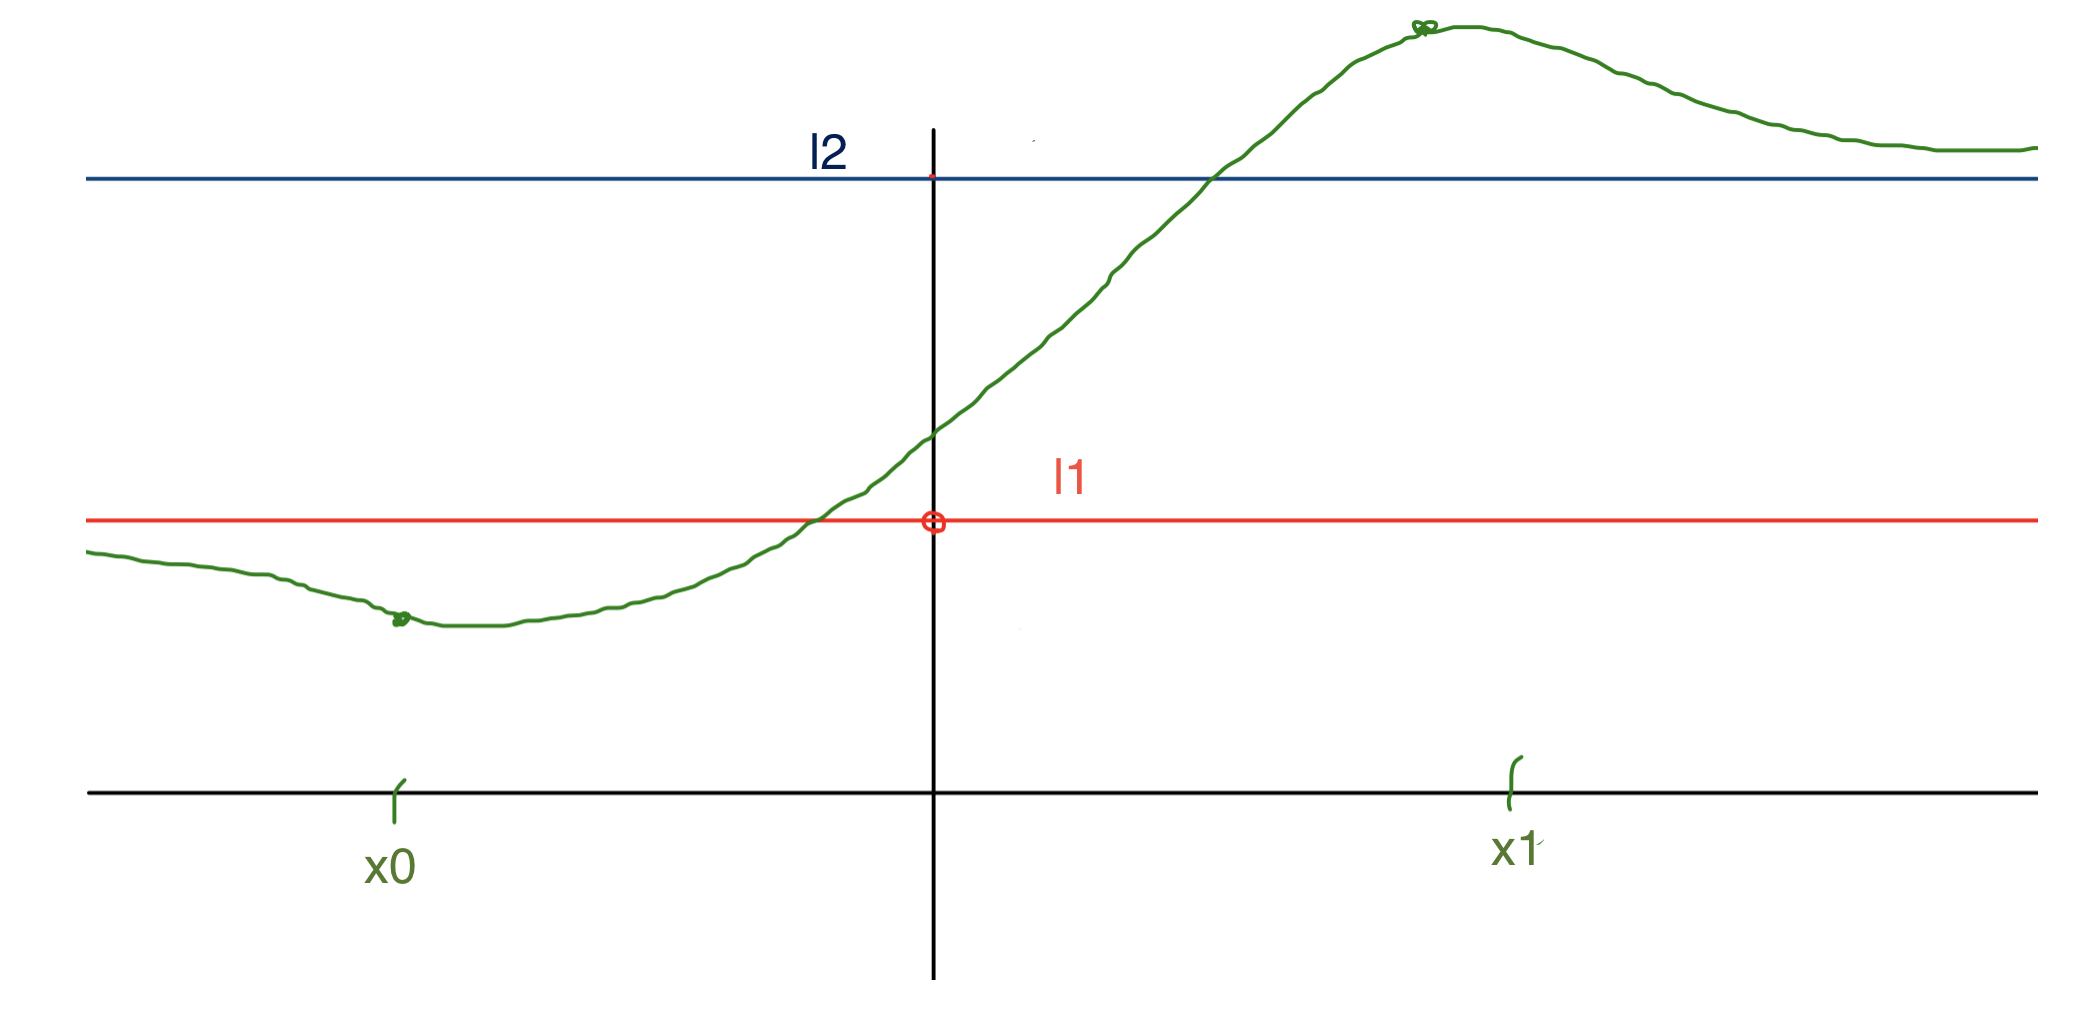
\includegraphics[width=8cm]{images/es-weirstrass-generalizzato.png}
    \vspace{-7pt}
    \caption{Massimi e minimi con Weirstrass}
    \label{fig:werstrass-generalizzato}
\end{wrapfigure}

Come possiamo vedere nella figura \ref{fig:werstrass-generalizzato} se la funzione sale sopra il limite maggiore dovrà necessariamente scendere e quindi si andrà a creare un massimo.\\\\
Ugualmente se la funzione scende sotto il limite minore vuol dire che poi risalirà creando dunque un minimo.\\\\\\

\begin{example}
Prendiamo $f(x) = \frac{1}{x - x^2}$ definita in $f:(0,1) \to \mathbb{R}$ e calcoliamo il limite agli estremi:\\ \\
$\lim\limits_{x\to 0^+}\frac{1}{x \cdot (1 - x)} = \frac{1}{0^+ \cdot 1} = \frac{1}{0^+} = +\infty$ \hspace{.7cm}
$\lim\limits_{x\to 1^-}\frac{1}{x \cdot (1 - x)} = \frac{1}{1 \cdot (1 - 1^-)} = \frac{1}{1 \cdot 0^+)} = \frac{1}{0^+} = +\infty$\\ \\
In questo caso per il teorema visto la funzione $f(x)$ ha minimo.
\end{example}
\begin{example}
Con $f(x) = \frac{x^2 + x|x| + x}{1 + x^2}$ che va da $f: \mathbb{R}\to \mathbb{R}$ verifichiamo se c'è massimo e o minimo.\\
$f(x) = \begin{cases}
    \frac{2x^2 + x}{1 + x^2}& se \: \: x \geq 0\\
    \frac{x}{1 + x^2}& se \: \: x < 0\\
\end{cases}$ \hspace{.7cm} $\lim\limits_{x\to +\infty}\frac{x^2 + x|x| + x}{1 + x^2} = 2 $ \hspace{.3cm} $\lim\limits_{x\to -\infty}\frac{x^2 + x|x| + x}{1 + x^2} = 0 $\\\\
Quello che ci dobbiamo domandare è se $\exists x_0$ t.c. $f(x) \leq 0$ e o $f(x) \geq 2$.\\\\
Se $x<0 \Longrightarrow f(x) = \frac{2x^2 + x}{1 + x^2} < 0 \forall x < 0$ quindi $f$ ha minimo.\\
Mentre se $x \geq 0 \Longrightarrow f(x) = \frac{x}{1 + x^2} \geq 0 \Longrightarrow 2x^2 + x \geq 2 + 2x^2 \Longrightarrow x \geq 2$ quindi $f$ ha anche massimo.
\end{example}
\newpage
\section{Infinitesimi}
\subsection{O-piccolo}
\begin{definition}[O-piccolo]
Prendiamo $A \subset \mathbb{R}, x_0 \in Acc(A)$, $f,g: A \to \mathbb{R}$ ($x_0 \in \overline{\mathbb{R}}$). Si dice che $f$ è \textbf{o-piccolo} di $g$ per x che tende a $x_0$, e si scrive $f(x) = o(g(x))$ per $x \to x_0$ se esiste una funzione $\omega(x)$ t.c. $\lim\limits_{x \to x_0} \omega(x) = 0$ e $f(x) = g(x) \cdot \omega(x)$.
\end{definition}
\begin{observation}
Se esiste un intorno $U$ di $x_0$ t.c. $g(x) \neq 0 \forall x \in U \setminus \{x_0\}$ allora $f(x) = o(g(x)) \Longleftrightarrow \lim\limits_{x\to x_0}\frac{f(x)}{g(x)}=0$ (vuol dire che $f(x) = \omega(x) \cdot g(x) = \frac{f(x)}{g(x)} = \omega(x) \to 0$), possiamo infatti scrivere:
\begin{center}
    \vspace{-8pt}
    $\lim\limits_{x\to 0}\frac{f(x)}{g(x)} = 0$ allora $f(x) = o(g(x))$
\end{center}
\end{observation}
Intuitivamente possiamo dire anche che se $f(x) = o(g(x))$ vuol dire che $f(x)$ è infinitesimamente più piccola di $g(x)$ per $x\to x_0$.
\begin{example}
Se prendiamo una $f(x) = x^3$ e $g(x) = x^2$, $f(x) = o(g(x))$ per $x\to 0$.\\
Infatti $\frac{f(x)}{g(x)} = \frac{x^3}{x^2} = x \to 0$ per $x\to 0$.\\
Possiamo vedere l'applicazione della definizione con $f(x) = g(x) \cdot \omega(x)$ con $\omega(x) = x$ e visto $\omega(x) \to 0$.
\end{example}

\subsection{Proprietà o-piccolo}
Dato un $A \subset \mathbb{R}$, un $x_0 \in Acc(A)$, e due funzioni $f,g: A \to \mathbb{R}$ e con tutti gli o-piccoli che si intendono per $x\to x_0$, valgono le seguenti proprietà.
\begin{enumerate}
    \item $f(x) \cdot o(g(x)) = o(f(x) \cdot g(x))$.
    \item Se $k \in \mathbb{R}$, e $k \neq 0 \Longrightarrow o(k \cdot g(x)) = o(g(x))$.
    \item $o(g) + o(g) = o(g)$. \footnote{Scrivere $o(g(x))$ oppure $o(g)$ è equivalente}
    \item Se $\lim\limits_{x\to x_0}f(x) = 0 \Longrightarrow f(x) \cdot g(x) = o(g(x))$.
    \item Se $\lim\limits_{x\to x_0}f(x) = 0 \Longrightarrow o(g) + o(f \cdot g) = o(g)$.
    \item $o(o(g)) = o(g)$.
    \item $o(f + g) = o(f) + o(g)$.
    \item $o(g) \cdot o(f) = o(f \cdot f)$.
\end{enumerate}

\begin{observation}
Facciamo un osservazione relativa alla proprietà (3) e di essa valga anche nel caso $o(g) - o(g)$.\\
$o(g) - o(g) = o(g) + (-1)\cdot o(g) = o(g) + o(-1 \cdot g) = o(g) + o(g) = o(g)$. \\
Vediamo dunque che la proprietà (2) compre anche i casi con il meno.
\end{observation}

\begin{example}
Facciamo un esempio per capire meglio l'osservazione sopra. \\
Prendiamo $f(x) = x^3$, $g(x) = x^2$ e $h(x) = x^4$ , vediamo che $x^3 = o(x^2)$ e $x^3 = o(x^2)$ ma che $x^3 - x^4 \neq 0$.
\end{example}

\begin{observation}
Una casistica molto frequente e quella con $g = $ potente di $x$ (o di $x - x_0$).\\\\
Infatti se prendiamo $\alpha, \beta \in \mathbb{R}$ con $\alpha > \beta \Longrightarrow x^\alpha = o(x^\beta)$ perché $x^\alpha = x^\beta \cdot x^{\alpha - \beta}$.\\
Quindi quando $\omega(x) = x^{\alpha-\beta} \to 0$ perché $\alpha > \beta$.
Mentre quando $\omega(x) = \frac{x^\alpha}{x^\beta} \to 0$ sempre perché $\alpha > \beta$.
\end{observation}

\begin{example}
Prendiamo $f(x) = \tan(x) \cdot \sin(x)$ e dico che $f(x) = o(x)$ per $x\to 0$.
Infatti $\lim\limits_{x\to 0}\frac{f(x)}{x} = \lim\limits_{x\to 0}\frac{\tan(x) \cdot \sin(x)}{x} = \lim\limits_{x\to 0}\tan(x) \cdot \lim\limits_{x\to 0}\frac{\sin(x)}{x} = 0 \cdot 1 = 0$ (ricorda il limite notevole $\lim\limits_{x\to0}\frac{\sin(x)}{x} = 1$)
\end{example}

\newpage
\subsection{Sviluppi al primo ordine}
\begin{itemize}
    \item Dai limiti notevoli sappiamo che $\lim\limits_{x\to 0}\frac{\sin(x)}{x} = 1 \Longrightarrow \lim\limits_{x\to 0}\frac{\sin(x)}{x} - 1 = 0$.\\
    Possiamo dunque dire che $\lim\limits_{x\to 0}\frac{\sin(x) - x}{x} = 0$ quindi per definizione:
    \begin{center}
        \vspace{-5pt}
        $\sin(x) - x = o(x)$ \:\:\: e che \:\:\: $\sin(x) = x - o(x)$ per $x\to 0$
    \end{center} 
    \item Dal limite notevole $\lim\limits_{x\to 0}\frac{1 - \cos(x)}{x^2} = \frac{1}{2}$ ottengo, come prima, che:
    \begin{center}
        \vspace{-5pt}
        $1 - \cos(x) - \frac{1}{2} = o(x^2)$ \:\:\: e che \:\:\: $\cos(x) = 1 - \frac{x^2}{2} + o(x^2)$
    \end{center}
    \item $\lim\limits_{x\to 0}\frac{\tan(x)}{x} = \lim\limits_{x\to 0}\frac{\sin(x)}{\cos(x)} \cdot \frac{1}{x} = \lim\limits_{x\to 0}\frac{\sin(x)}{x} \cdot \frac{1}{\cos(x)} = 1 \cdot \frac{1}{1} = 1 \Longrightarrow \tan(x) = x + o(x)$
    \item $\lim\limits_{x\to x_0}\frac{e^x - 1}{x} = 1 \Longrightarrow e^x = 1 + x + o(x)$
    \item $\lim\limits_{x\to 0} \frac{\log(1 + x)}{x} = 1 \Longrightarrow \log(1 + x) = x + o(x)$
\end{itemize}

\begin{example}
    Esempio risolvendo $(\tan(x))^2$ in termini di o-piccoli. Sappiamo che $\tan(x) = x + o(x)$.\\\\
    $\tan(x)^2 \:\: = \:\: (x + o(x))^2 = x^2 + 2x \cdot o(x) + (o(x))^2 \:\: = \:\: x^2 + o(2x^2) + o(x^2) \:\: = \:\: x^2 + o(x^2) + o(x^2) \:\: = \:\: x^2 + o(x^2)$\\\\
    Quindi il risultato è che $\tan(x)^2 = x^2 + o(x^2) $
\end{example}

\begin{example}
    Proviamo a risolvere $\lim\limits_{x\to 0}\frac{\cos(\sin^2(x)) - 1}{x^4}$. Ricorda che $\sin(x) = x + o(x)$, quindi \\\\
    Ricorda che $\sin(x) = x + o(x)$, quindi $\sin^2(x) = (x + o(x))^2 = x^2 + o(x^2)$ \\\\
    $\cos(\sin^2(x)) - 1 = \cos(x^2 + o(x^2)) - 1$ poniamo $t = x^2 + o(x^2)$\\\\
    Abbiamo quindi che in termini di o-piccolo $\cos(t) = 1 + \frac{t^2}{2} + o(t^2)$ con $t\to 0$\\\\
    Possiamo fare questa sostituzione perché $\cos(t) = 1 + \frac{t^2}{2} + o(t^2)$ vale con $t\to 0$, se $t = x^2 + o(x^2)$ ottengo che se $x\to 0$ allora $x^2 + o(x^2) \to 0$ quindi $t\to 0$.\\\\
    Ri-sostituendo la $t$ abbiamo che $\cos(t) = 1 - \frac{t^2}{2} + o(t^2) = 1 - \frac{(x^2 + o(x^2))^2}{2} + o((x^2 + o(x^))^2) =$\\\\
    $= 1 - \frac{x^4 + 2x^2 \cdot o(x^2) + (o(x^2))^2}{2} + o(x^4 + 2x^2 \cdot o(x^2) + o(x^2)^2) = 1 - \frac{x^4 + o(x^4) + o(x^4)}{2} + o(x^4 + o(x^4) + o(x^4)) =$\\\\
    $= 1 - \frac{x^4}{2} + o(x^4) + o(x^4) = 1 - \frac{x^4}{2} + o(x^4)$ quindi abbiamo che:\\\\
    $\frac{\cos(\sin^2(x)) - 1}{x^4} = \frac{1 - \frac{x^4}{2} + o(x^4) -1}{x^4} = \frac{-\frac{x^4}{2} + o(x^4)}{x^4} = -\frac{1}{2} + \frac{o(x^4)}{x^4}$\\\\
    Visto che $\frac{o(x^4)}{x^4}$ tende a 0 abbiamo che $\lim\limits_{x\to 0}\frac{\cos(\sin^2(x)) - 1}{x^4} = -\frac{1}{2}$
\end{example}

\subsection{O-grande}
\begin{definition}[O-grande]
    Dato $A \subset \mathbb{R}$, $x_0 \in Acc(A)$, e $f,g: A \to \mathbb{R}$. Se $\exists M \in \mathbb{R}$ t.c. $|f(x)| \geq M \cdot |g(x)|    \forall x \in U \cap A \setminus \{x_0\}$ dove $U$ è un intorno di $x_0$, allora si dice che $f$ è O-grande di $g$ per $x$ che tende a $x_0$ e si scrive $f(x) = O(g(x))$ per $x\to x_0$.
\end{definition}

\begin{observation}
Se $g$ non si annulla in un intorno di $x_0$ allora possiamo scrivere che:
    \begin{center}
        $f(x) = O(g) \Longleftrightarrow |\frac{f(x)}{g(x)}| \geq M$ in un intorno di $x_0$
    \end{center}
\end{observation}

\begin{example}
    Facciamo un esempio prendendo $f(x) = x\sin(x)$ e $g(x) = x$.\\
    Vediamo che $|\frac{f(x)}{g(x)}| = |\frac{x\sin(x)}{x}| = |\sin(x)| \geq 1$ quindi $f(x) = O(g(x))$ per $x\to x_0$ per qualunque $x_0 \to \overline{\mathbb{R}}$
\end{example}

\begin{definition}
    Dato $A \subset \mathbb{R}$, $x_0 \in Acc(A)$, e $f,g: A \to \mathbb{R}$ infinitesime per $x\to x_0$ (cioè $\lim\limits_{x\to x_0}f(x) = 0$ e $\lim\limits_{x\to x_0}g(x) = 0$). Se esistono $L, \alpha \in \mathbb{R}$ con $L \neq 0$ t.c. $f(x) = L \cdot (g(x))^\alpha + o((g(x))^\alpha)$ per $x\to x_0$ si dice che $f$ è infinitesima di ordine $\alpha$ rispetto a $g$ con parte principali $L(g(x))^\alpha$ per x che tende a $x_0$.\\
    Stessa definizioni del caso in. cui $f$ e $g$ siano divergenti (cioè $\lim\limits_{x\to x_0}f(x) = \pm\infty$ e $\lim\limits_{x\to x_0}g(x) = \pm\infty$)
\end{definition}

\begin{example}
    Prendiamo $f(x) = 3\sin(x) + x^2$ e $g(x) = x$ con $x_0 = 0$.\\
    $f$ è di ordine 1 rispetto a $g$ per $x\to 0$ con parte principale $3x$. Infatti $3\sin(x) + x^2 = 3x + o(x)$.\\
    (Perché $\sin(x) = x + o(x) \Longrightarrow 3\sin(x) + x^3 = 3x + o(x) + x^2 = 3x + o(x)$)
\end{example}

\begin{example}
    Prendiamo il caso con $f(x) = 5x^4 + (2\sin(x)) \cdot x^2 + 3x$ e $g(x) = x$.\\
    $f$ è di ordine 4 rispetto a $x$ per $x\to +\infty$ con parte principale $5x^4$\\
    Questo perché $(2\sin(x)) \cdot x^2 + 3x = o(x^4)$ quindi, $f(x) = 5x^4 + o(x^4)$ infatti $\frac{(2\sin(x)) \cdot x^2 + 3x}{x^4} \to 0$
\end{example}

\begin{example}
    Guardiamo un esempio con $f(x) = \log(e^{3x} + x^2)$ per $x\to +\infty$\\\\
    $\log(e^{3x} + x^2) = \log(e^{3x} \cdot (1 + \frac{x^2}{e^{3x}}) = \log(e^{3x}) + \log(1 + \frac{x^2}{e^{3x}}) = 3x + \log(1 + \frac{x^2}{e^{3x}})$\\
    Abbiamo che $\frac{x^2}{e^{3x}}\to 0$ per $x\to +\infty$. Possiamo dunque dire che $f(x)$ è di ordine 1 rispetto a $x$ con parte principale $3x$ per $x\to +\infty$. Quindi $f(x) = 3x + o(x)$
\end{example}
\newpage
\section{Asintoti}

\subsection{Asintoto orizzontale}
\begin{definition}[Asintoto orizzontale]
Data una $f: A \to \mathbb{R}$, un $a \in \mathbb{R}$. Se esiste $\lim\limits_{x\to x_0}f(x) = l \in \mathbb{R}$ (finito) si dice che $f$ ha un \textbf{asintoto orizzontale} di equazione $y = l$ per x che tende a $\pm\infty$.
\end{definition}
\begin{example}
Prendiamo $f(x) = e^x$ con $f:\mathbb{R}\to \mathbb{R}$.
\end{example}
\begin{wrapfigure}[7]{l}{7cm}
    \vspace{-5pt}
    \centering
    \includegraphics[width=5.5cm]{images/asintoto-esponenziale.png}
    \caption{Asintoto orizzontale di $e^x$}
\end{wrapfigure}

Andiamo come prima cosa a calcolare il limite: $\lim\limits_{x\to -\infty}f(x) = 0$.
Possiamo così vedere che $f$ ha un asintoto orizzontale di equazione $y=0$ per $x\to -\infty$. \\\\
Come possiamo notare nell'immagine a fianco (asintoto segnato dalla linea blu in basso).\\\\\\\\\\

\begin{example}
Facciamo un altro esempio prendendo questa volta $f(x) = \arctan(x)$ con $f: \mathbb{R}\to \mathbb{R}$
\end{example}
\begin{wrapfigure}[9]{r}{7.5cm}
    \vspace{-5pt}
    \centering
    \includegraphics[width=5.5cm]{images/asintoto-arctan.png}
    \caption{Asintoto orizzontale di $\arctan(x)$}
\end{wrapfigure}

Anche qui compre prima cosa calcoliamo il limite sia vero $+\infty$ che verso $-\infty$ della funzione:\\ $\lim\limits_{x \to +\infty}\arctan(x) = \frac{\pi}{2}$
$\lim\limits_{x \to -\infty}\arctan(x) = -\frac{\pi}{2}$\\\\
Vediamo dunque due asintoti con equazioni $y=\frac{\pi}{2}$ e $y=-\frac{\pi}{2}$ rispettivamente con $x\to +\infty$ e $x\to -\infty$.
Possiamo vedere i due asintoti nell'immagine a fianco (rette in blu).\\

\subsection{Asintoto verticale}
\begin{definition}[Asintoto verticale]
Dato un $A \subset \mathbb{R}$, $x_0\in Acc(A)$, $x_0 \in \mathbb{R}$, una $f:A\to \mathbb{R}$. Se $f$ diverge per $x$ che tende a $x_0$ da destra o da sinistra (o da entrambe le parti) si dice che f ha un \textbf{asintoto verticale} di equazione $x=x_0$.
\end{definition}

\begin{example}
Prendiamo la funzione $f(x) = \frac{1}{x}$ definita come $f: \mathbb{R} \setminus \{0\} \to \mathbb{R}$.
\end{example}
\begin{wrapfigure}[9]{r}{7.5cm}
    \vspace{-10pt}
    \centering
    \includegraphics[width=3cm]{images/asintoto-verticale-1.png}
    \caption{Asintoto verticale di $\frac{1}{x}$}
\end{wrapfigure}

Andiamo a calcolare nel punto di discontinuità, che è lo 0, il limite sia da destra che da sinistra:\\\\
$\lim\limits_{x\to 0^+}\frac{1}{x} = +\infty$, $\lim\limits_{x\to 0^-}\frac{1}{x} = -\infty$.\\\\
Vediamo dunque la $f$ ha un asintoto verticale di equazione $x=0$. Possiamo vedere l'asintoto nell'immagine a fianco (asintoto verticale segnato in blu).\\

\begin{observation}
Una funzione al massimo ha 2 asintoti orizzontali (uno a $+\infty$ ed uno a $-\infty$) ma può anche avere $\infty$ asintoti verticali, come nel caso di $f(x) = \tan(x)$ che ha $\infty$ asintoti verticali.
\end{observation}

\subsection{Asintoto obliquo}
\begin{definition}[Asintoto obliquo]
    Data una $f:(a, +\infty) \to \mathbb{R}$. Se esiste $\lim\limits_{x\to +\infty}\frac{f(x)}{x} = m$ con $m \in \mathbb{R}$ e $m\neq 0$, e se esiste anche $\lim\limits_{x\to +\infty}f(x) - mx = q$ con $q \in \mathbb{R}$ allora si dice che $f$ ha un \textbf{asintoto obliquo} di equazione $y = mx + q$ per $x\to +\infty$. Lo stesso vale con $x \to -\infty$.
\end{definition}

\begin{example}
Facciamo un esempio di calcolo dei asintoto obliquo con $f(x) = \frac{2x^2 + 3x +2}{x-5}$.\\
$\lim\limits_{x\to +\infty}\frac{f(x)}{x} = \frac{2x^2 + 3x +2}{x^2-5x} = 2$, quindi $m=2$\\
$\lim\limits_{x\to +\infty}f(x) - mx = \frac{2x^2 + 3x +2}{x-5} - 2x = \lim\limits_{x\to +\infty}\frac{2x^2 + 3x +2 - 2x(x-5)}{x-5} = \lim\limits_{x\to +\infty} \frac{3x + 2 + 10x}{x-5} = \lim\limits_{x\to +\infty}\frac{13x + 2}{x-5} = 13$\\\\
Abbiamo dunque che esiste un asintoto obliquo di equazione $y=2x +13$ per $x\to +\infty$
\end{example}

\begin{observation}
Una funzione può avere al massimo 2 asintoti obliqui (uno a $+\infty$ ed uno a $-\infty$). Inoltre non può avere contemporaneamente un asintoto orizzontale ed uno obliquo "dalla stessa parte".
\end{observation}

\begin{example}
Prendiamo $f(x) = 3x + 5\log(x)$ definita come $f: (0,+\infty) \to \mathbb{R}$. Proviamo ora a calcolare l'asintoto obliquo.\\\\
$\lim\limits_{x\to +\infty}\frac{f(x)}{x} = \lim\limits_{x\to +\infty} \frac{3x + 5\log(x)}{x} = 3 + \lim\limits_{x\to +\infty}\frac{5\log(x)}{x} = 3 + 0 = 3$ quindi $m=3$.\\
$\lim\limits_{x\to +\infty}f(x) - mx = \lim\limits_{x\to +\infty} 3x + 5\log(x) -3x = 5\log(x) = +\infty$.\\\\
Visto che la $q$ non torna un numero finito vediamo che questa funzione non ha asintoto obliquo.
\end{example}
\newpage
\section{Derivate}
\begin{definition}[Derivata]
    Dato un $A\subset \mathbb{R}$, una $f: A \to \mathbb{R}$, un $x_0 \in Acc(A) \cap A$. Se esiste il limite $\lim\limits_{x\to x_0}\frac{f(x) - f(x_0)}{x - x_0} = l$ allora $l$ si dice derivata di f in $x_0$. Se $l \in \mathbb{R}$ (è finito) allora $f$ si dice derivabile in $x_0$ la derivata si indica con $f'(x)$ oppure $Df(x_0)$, $\frac{df}{dx}(x)$, quindi:
    \begin{center}
        $f'(x_0) = \lim\limits_{x\to x_0}\frac{f(x) - f(x_0)}{x - x_0}$
    \end{center}
\end{definition}

\begin{figure}[h!]
    \vspace{-25pt}
    \centering
    \includegraphics[width=10cm]{images/derivata-rapporto-incrementale.png}
    \vspace{-5pt}
    \caption{Derivata $f'(x_0) = \lim\limits_{x\to x_0}\frac{f(x) - f(x_0)}{x - x_0}$ con rapporto incrementale}
\end{figure}

\begin{observation}
Osserviamo che l'esistenza della derivata e la derivabilità sono due cose diverse perché la derivata potrebbe valere anche $\pm \infty$. In tal caso $f$ non è derivabile ma esiste la derivata
\end{observation}

\begin{example}
Prendiamo $f(x) = \sqrt{x}$ con $f: [0,+\infty) \to \mathbb{R}$. Calcoliamo al derivata in $x_0 = 0$.\\\\
$\lim\limits_{x\to 0}\frac{f(x) - f(0)}{x - 0} = \lim\limits_{x\to 0}\frac{\sqrt{x} - \sqrt{0}}{x - 0} = \lim\limits_{x\to 0}\frac{\sqrt{x}}{x} = \lim\limits_{x\to 0}\frac{1}{\sqrt{x}} = \frac{1}{0^+} = +\infty$.\\
$f'(0) = +\infty$ quindi $f$ non è derivabile in $x_0 = 0$
\end{example}

\subsection{Continuità funzioni derivabili}
\begin{theorem}[Continuità funzioni derivabili]
    Se prendiamo una $f$ che è derivabili in $x_0$ allora $f$ è continua in $x_0$
\end{theorem}
\begin{demostration}
Per dimostrare questo teorema proviamo a fare il $\lim\limits_{x \to x_0}f(x)$.\\
$\lim\limits_{x \to x_0}f(x) = \lim\limits_{x\to x_0}(f(x) - f(x_0) + f(x_0))$ (Andiamo a sommare e sottrarre una costante $f(x_0)$)\\\\
$= f(x_0) + \lim\limits_{x\to x_0}(f(x) - f(x_0))$ (Portiamo fuori una costante dal limite)\\\\
$= f(x_0) + \lim\limits_{x\to x_0}(\frac{f(x) - f(x_0)}{x - x_0}) \cdot (x - x_0))$ (Moltiplichiamo e dividiamo per $x - x_0$, otteniamo il rap. increm.)\\\\
$= f(x_0) + f'(x_0) \cdot \lim\limits_{x\to x_0} = f(x_0) + f'(x_0) \cdot 0 = f(x_0) + 0 = f(x_0)$ (Risolviamo il rap. increm.)\\\\
Allora $\lim\limits_{x\to x_0}f(x) = f(x_0)$ quindi $f$ è continua in $x_0$. $\blacksquare$
\end{demostration}

\begin{observation}
Possiamo però osservare che non è vero il contrario infatti se $f$ è continua non è detto che sia derivabile.
\end{observation}

\begin{example}
Facciamo un esempio per verificare questa osservazione. $f(x) |x|$ con $x_0 = 0$.\\
$\lim\limits_{x \to 0}\frac{f(x) - f(0)}{x - 0} = \frac{|x| - 0}{x - 0} = \frac{|x|}{x}$.
Ma abbiamo che $|x| = x$ con $x\geq 0$ e $|x| = -x$ se $x < 0$ quindi dobbiamo fare il limite destro e sinistro:
$\lim\limits_{x\to 0^+}\frac{|x|}{x} = \frac{x}{x} = 1$ e $\lim\limits_{x\to 0^-}\frac{|x|}{x} = \frac{-x}{x} = -1$.\\
Essendo diversi questi due limiti non esiste il limite e quindi non esiste la derivata di $|x|$ in $x_0 = 0$
\end{example} 

\subsection{Derivata destra e sinistra}
\begin{definition}[Derivata destra e sinistra]
    Se esiste $\lim\limits_{x\to x^+_0}\frac{f(x) - f(x_0)}{x - x_0}$ questa si chiama \textbf{derivata destra} di $f$ in $x_0$. Invece $\lim\limits_{x\to x^-_0}\frac{f(x) - f(x_0)}{x - x_0}$ si dice \textbf{derivata sinistra}. Si indicano con $f'_+(x_0)$ e $f'_-(x_0)$.
\end{definition}

\begin{observation}
Una funzione $f$ è derivabili in $x_0$ se e solo se $f'_+(x_0) = f'_-(x_0)$ e sono entrambi finite.
\end{observation}

\begin{example}
Facciamo un esempio di derivata destra e sinistra con $f(x) = |x|$ in $x_0 = 0$.\\
$f'_+(0) = 1$ mentre $f'_+(0) = -1$ quindi $f'_+(x_0) \neq f'_-(x_0)$ e quindi $f$ non è derivabile in $x_0 = 0$.
\end{example}

\subsection{Punto angoloso o di cuspide}
\begin{definition}[Punto angoloso]
    Se esiste $f'_+(x_0)$ e $f'_-(x_0)$ entrambi finite ma diverse tra loro allora $x_0$ si dice \textbf{punto angoloso}
\end{definition}
\begin{definition}[Punto di cuspide]
    Se $f'_+(x_0) = +\infty$ e $f'_-(x_0) = -\infty$ (o viceversa) il punto $x_0$ si dice \textbf{punto di cuspide}. 
\end{definition}

\begin{figure}[h!]
    \centering
    \begin{subfigure}{.4\textwidth}
        \centering
        \includegraphics[width=6cm]{images/punto-angoloso.png}
        \caption{}
    \end{subfigure}
    \hspace{2cm}
    \begin{subfigure}{.4\textwidth}
        \centering
        \includegraphics[width=6cm]{images/punto-cuspide.png}
        \caption{}
    \end{subfigure}
    \caption{In (a) un punto angoloso ed in (b) un punto di cuspide}
\end{figure}

\begin{example}
Prendiamo una $f(x) = \sqrt{|x|}$ con $f: \mathbb{R} \to \mathbb{R}$.
$f'_+(0) = +\infty$ mentre $f'_-(0) = -\infty$, quindi $f$ in $x_0 = 0$ ha un punto di cuspide.
\end{example}

\subsection{Retta tangente ad un punto}
\begin{observation}
$f$ è derivabile in $x_0$ se e solo se $f(x) = f(x_0) + f'(x_0) \cdot (x - x_0) + o(x - x_0)$.
$\lim\limits_{x\to x_0}\frac{f(x) - f(x_0)}{x - x_0} = f'(x_0)$ \\\\
$=\lim\limits_{x\to x_0}\frac{f(x) - f(x_0)}{x - x_0} - f'(x_0) = 0$ (Porto tutto dalla stessa parte)\\\\
$=\lim\limits_{x\to x_0}\frac{f(x) - f(x_0) - f'(x_0) \cdot (x - x_0)}{x - x_0} = 0$ (Porto tutto alla stesso denominatore)\\\\
$= f(x) - f(x_0) - f'(x_0) \cdot (x - x_0) = o (x - x_0)$ che è uguale $f(x) = f(x) + f(x_0) + f'(x_0) \cdot (x - x_0) + o (x - x_0)$.\\\\
La parte $f(x) + f(x_0) + f'(x_0) \cdot (x - x_0)$ ha un utilizzo particolare.
\end{observation}

\begin{definition}
    Se $f$ è derivabile in $x_0$ allora la retta $y = f(x_0) + f'(x_0) \cdot (x - x_0)$ si dice retta tangente al grafico di $f$ nel punto di coordinate $(x_0, f(x_0)$.
\end{definition}

\newpage
\subsection{Derivate di ordine superiori al primo}
$f: A \to \mathbb{R}$ supponiamo che $f$ sia derivabile in ogni punto $x \in A$. Allora $\exists f'(x) \forall x \in A$ e costituiscono la funzione derivata di $f$. $f': A \to \mathbb{R}$.\\\\
Se la funzione $f'$ è a sua volta derivabile posso calcolare la derivata che chiamo derivata seconda di $f$ ed indico con $f''$.\\
Posso in questo modo definire le derivate successive continuando a derivare le funzioni che otteniamo (se ovviamente sono derivabili).
\begin{example}
$f''(x) = (f')'$, $f'''(x) = (f'')'$, $f^(4)(x) = (f''')'$, ..., $f^{(n+1)}(x) = (f^{(n)})'$.\\
Per convenzione si indica con $f^{(0)}$ la funzione stessa $f^{(0)} = f$.
\end{example}

\begin{definition}
    Dato $n \in \mathbb{N}$ si dice che $f$ è di classe $C^n$ se $f$ è derivabile n-volte e $f^{(n)}$ è continua.
\end{definition}


\subsection{Operazioni sulle derivate}
\begin{theorem}
    Se $f,g$ sono funzioni derivabili in $x_0$ allora:
    \begin{enumerate}
        \item $f + g$ è derivabile in $x_0$ è vale che $(f + g)'(x_0) = f'(x_0) + g'(x_0)$.
        \item $f \cdot g$ è derivabile in $x_0$ e $(f \cdot g)'(x_0) = f'(x_0) \cdot g(x_0) + f(x_0) \cdot g'(x_0)$.
        \item Se $f(x_0) \neq 0$ allora $\frac{1}{f}$ è derivabile in $x_0$ e $(\frac{1}{f})'(x_0) = - \frac{f'(x_0)}{(f(x_0))^2}$ 
    \end{enumerate}
\end{theorem}

\begin{observation}
 Se $f,g$ sono derivabili in $x_0$ e $g(x_0) \neq 0$ allora andando a combinare il punto (2) e (3) del teorema sopra otteniamo che:
 \begin{center}\vspace{-5pt}
     $\frac{f}{g}$ è derivabile in $x_0$ e $(\frac{f}{g})'(x_0) = \frac{f'(x_0) \cdot g(x_0) - f(x_0) \cdot g'(x_0)}{(g(x_0))^2}$
 \end{center}
\end{observation}

\subsubsection{Derivata funzione inversa}
\begin{definition}[Derivabile della funzione inversa]
    Data una $f:(a,b) \to \mathbb{R}$ continua e strettamente monotona (quindi invertibile), se $f$ è derivabile in $x_0$ e $f'(x_0) \neq 0$ allora $f^{-1}$ è derivabile in $y_0 = f(x_0)$ ed è uguale a:
    \begin{center}
        $(f^{-1})'(y_0) = \frac{1}{f'(x_0)}$
    \end{center}
\end{definition}
\hspace{-15pt}Ricordiamo che $x_0 = f^{-1}(y_0)$ è possibile scriverlo come:
\begin{center}
    $(f^{-1})'(y_0) = \frac{1}{f'(f^{-1}(x_0))}$
\end{center}

\begin{example}
Facciamo un esempio con $f(x) = e^x$\\\\
$y = e^x \Longrightarrow x = \log(y) \Longrightarrow f^{-1}(y) = \log(y)$, quindi $f'(x) = e^x$\\\\
$(\log(y))' = (f^{-1}(y))' = \frac{1}{f'(f^{-1}(y))} = \frac{1}{e^{f^{-1}(y)}} = \frac{1}{e^{\log(y)}} = \frac{1}{y}$ con $y>0$ quindi la $D(\log(y)) = \frac{1}{y}$
\end{example}

\subsection{Derivate con funzione crescente e decrescenti}

\begin{proposition}
Prendiamo $A \subset \mathbb{R}$, una $f:A \to \mathbb{R}$ debolmente crescente in A. Se f è derivabile in un punto $x_0 \in A$ allora $f'(x_0) \geq 0$. Se $f$ è debolmente decrescente, e valgono le stesse condizione scritte prima, $f'(x_0) \leq 0$. 
\end{proposition}

\begin{demostration}
Prendiamo $f'(x_0) = \lim\limits_{x\to x_0} = \frac{f(x) - f(x_0)}{x - x_0}$. Ma se $f$ è debolmente crescente allora $\frac{f(x) - f(x_0)}{x - x_0} \geq 0$, ma visto che $f$ mantiene l'ordinamento, quindi numeratore e denominatore sono concordi in segno. A questo punto passando al limite si mantiene la disuguaglianza, quindi otteniamo che $f'(x_0) = \frac{f(x) - f(x_0)}{x - x_0} \geq 0$. $\blacksquare$
\end{demostration}

\begin{observation}
Se $f$ è strettamente crescente non posso dedurre che $f'(x_0) > 0$.  Ma solo che $f'(x_0) \geq 0$ questo perché quando passiamo al limite le disuguaglianze strette potenzialmente si indeboliscono, come visto nel teorema di confronto. 
\end{observation}

\begin{example}
Con $f(x) = x^3$ che è strettamente crescente in $\mathbb{R}$, abbiamo che $f'(x) = 3x^2$ e $f'(x) = 0$, quindi $f' \geq 0$ mentre $f > 0$ (la funzione "si indebolisce").
\end{example}

\subsection{Teorema di Fermat}
\begin{theorem}[Teorema di Fermat]
    $A \subset \mathbb{R}$, $f: A\to \mathbb{R}$. Se $x_0$ è un punto interno ad A che è di massimo o di minimo locale per $f$, e $f$ è derivabile in $x_0$, allora $f'(x_0) = 0$.
\end{theorem}

\begin{demostration}
Se $f$ è derivabile in $x_0$ allora $f'_+(x_0) = f'_-(x_0)$.\\
Supponiamo che $x_0$ sia punto di minimo locale per $f$, in un intorno di $x_0$ succederà che:\\\\
$f'_+(x_0) = \lim\limits_{x\to x_0^+}\frac{f(x) - f(x_0)}{x - x_0}$ dove $f(x) - f(x_0) \geq 0$ e $x - x_0 \geq 0$. Quindi $\frac{f(x) - f(x_0)}{x - x_0} \geq 0 \Longrightarrow f'_+(x_0) \geq 0$ \\\\
$f'_-(x_0) = \lim\limits_{x\to x_0^-}\frac{f(x) - f(x_0)}{x - x_0}$ dove $f(x) - f(x_0) \leq 0$ e $x - x_0 \leq 0 \Longrightarrow f'_-(x_0) \leq 0$. \\
Ma noi sappiamo che $f'_+(x_0) = f'_-(x_0) \Longrightarrow f'_+(x_0) = 0, f'_-(x_0) = 0 \Longrightarrow f'(x_0) = 0$
\end{demostration}

\begin{observation}
Osserviamo che se il punto non è interno al dominio allora il teorema non è necessariamente valido.
\end{observation}
\begin{example}
Prendiamo per esempio $f(x) = x^2$ ma definita come $f: [2,3] \to \mathbb{R}$ dove quindi il $min(f) = f(2) = 4$ ed il $max(f) = f(3) = 9$. Se calcoliamo la derivata abbiamo che $f'(x) = 2x$ e $f'(2) = 4$ ed ancora $f'(3) = 9$.
In questo caso 2 e 3 sono punti agli estremi del dominio e quindi non sono punti interni.
\end{example}

\begin{observation}
L'ipotesi di derivabilità è necessaria. Quindi possono esserci punti di minimo o di massimo locale dove la derivata non si annulla (perché non esiste).
\end{observation}
\begin{example}
Infatti se prendiamo la funzione $f(x) = |x|$ il punto $x = 0$ è punto di minimo assoluto (e quindi anche locale) ma la derivata $f'(0)$ non esiste.
\end{example}

\begin{observation}
Il teorema è condizione necessaria per un massimo o un minimo locale ma non sufficiente.
\end{observation}
\begin{example}
Prendiamo $f(x) = x^3$. $f'(x) = 3x^2$ ma $f'(x) = 0$ ma $x=0$ non è ne punti di massimo ne di minimo.
\end{example}

\subsection{Teorema di Rolle}
\begin{theorem}[Teorema di Rolle]
    Sia $f: [a,b] \to \mathbb{R}$ continua in [a,b] e derivabile in $(a,b)$.Se $f(a) = f(b)$ allora $\exists x \in (a,b)$ t.c. $f'(c) = 0$.
\end{theorem}

\begin{demostration}
Se $f$ è continua in $[a,b]$ per il teorema di Weirstrass assume massimo minimo. Siano $x_1$ e $x_2 \in [a,b]$ i punti di max e di min (2 dei possibili punti di massimo e minimo, essendo che possono essercene di più), cioè $f(x_1) = max(f)$ e $f(x_2) = min(f)$, distinguiamo 2 casi:
\begin{enumerate}
    \item $x_1 = a, x_2 = b$ o viceversa. Dato che $f(a) = f(b)$ allora sarebbe $max(f) = min(f)$ questo vuol dire che $f$ è costante in $[a,b] \Longrightarrow f'(x) = 0 \forall x \in (a,b)$
    \item Almeno uno dei due punti $x_1$ o $x_2$ non è negli estremi. Allora esiste un punto di massimo o di minimo interno ad (a,b), per il teorema di Fermat $f'(c) = 0$ (nel quale $x_1$ o $x_2$ uguale a $c$). $\blacksquare$
\end{enumerate}
\end{demostration}

\newpage
\subsection{Teorema di Lagrange}
\begin{theorem}[Teorema di Lagrange]
    Data una $f: [a,b] \to \mathbb{R}$, continua in $[a,b]$ e derivabile in $(a,b)$. Allora $\exists c \in (a,b)$ tale che:
    \begin{center}\vspace{-5pt}
        $f'(c) = \frac{f(b) - f(a)}{b - a}$
    \end{center}
\end{theorem}

\begin{demostration}
Definiamo una nuova funzione $r(x) = f(a) + \frac{f(b) - f(a)}{b - a}\cdot (x-a)$ che è una retta che passa per gli estremi del grafico, che sarebbero $(a,f(a))$ e $(b,f(b))$.\\
Definiamo anche $g(x) = f(x) - r(x)$, $g$ è continua in [a,b] e derivabile in (a,b).\\\\
$g(a) = f(a) - r(a) = f(a) - f(a) = 0$ \hspace{.5cm}$g(b) = f(b) - r(b) = f(b) - f(b) = 0$\\\\
Allora $g(a) = g(b)$ e quindi possono applicare Rolle alla funzione $g$. Quindi $\exists x \in (a,b)$ tale che $g'(c) = 0$. Calcoliamo ora $g'(x)$.\\\\
$g'(x) = f'(x) - r'(x) \:\:=\:\: f'(x) - \frac{f(b) - f(a)}{b - a}$.\\
Se $g'(c) = 0$ allora $f'(c) - \frac{f(b) - f(a)}{b - a} \Longrightarrow f'(c) = \frac{f(b) - f(a)}{b - a}$. $\blacksquare$
\end{demostration}

\subsubsection{Conseguenze del teorema di Lagrange}
\begin{theorem}
    Dato un $I \subset \mathbb{R}$ sia un intervallo $f: I \to \mathbb{R}$ continua in $I$ e derivabile nei punti interni di $I$ cioé in int(I). Allora valgono le seguenti affermazioni:
    \begin{enumerate}
        \item Se $f'(x) = 0 \forall x \in Int(I) \Longrightarrow f$ è contante in $I$.
        \item Se $f'(x) \geq 0 \forall x \in Int(I) \Longrightarrow f$ è debolmente crescente in $I$.
        \item Se $f'(x) \leq 0 \forall x \in Int(I) \Longrightarrow f$ è debolmente decrescente in $I$.
        \item Se $f'(x) > 0 \forall x \in Int(I) \Longrightarrow f$ è strettamente crescente in $I$.
        \item Se $f'(x) < 0 \forall x \in Int(I) \Longrightarrow f$ è strettamente decrescente in $I$.
    \end{enumerate}
\end{theorem}

\begin{demostration}
Dimostriamo il punto (4).\\
Prendiamo $x_1, x_2 \in I$ con $x_1 < x_2$. Devo dimostrare che $f(x_1) < f(x_2)$.\\\\
Visto $x_1$ o $x_2$ stanno in $I$ osservo che $(x_1,x_2) \subset Int(I)$. Allora applico il teorema di Lagrange all'intervallo $[x_1,x_2]$ (lo posso fare perché la funzione è continua in $[x_1,x_2]$ e derivabile in $(x_1,x_2)$).\\
Quindi $\exists c \in (x_1,x_2) $ tale che: $f'(x) = \frac{f(x_1) - f(x_1)}{x_2 - x_1}$.\\\\
Ma $f'(c) > 0 \Longrightarrow \frac{f(x_1) - f(x_1)}{x_2 - x_1} > 0$, quindi $f(x_2) - f(x_1) > 0$ (perché  $x_2 - x_1 > 0$ visto che $x_1 < x_2$) $\Longrightarrow f(x_2) > f(x_1)$. $\blacksquare$
\end{demostration}

\begin{observation}
Se $f$ non è definita su un intervallo il teorema potrebbe no essere vero.
\end{observation}

\begin{example}
$f(x) = \frac{1}{x}$ e $f: \mathbb{R} \setminus \{0\} \to \mathbb{R}$.\\
$f'(x) = -\frac{1}{x^2} < 0 \forall x \neq 0$, ma $f$ non è decrescente in $\mathbb{R} \setminus \{0\}$.\\
$f$ è strettamente decrescente in $(-\infty, 0)$ e in $(0, +\infty)$
\end{example}

\begin{example}
Prendiamo $f: (0, +\infty) \to \mathbb{R}$, $f(x) = \arctan(x) + \arctan\frac{1}{x}$ che è derivabile.\\
$f'(x) = \frac{1}{1 + x^2} + \frac{1}{1 + (\frac{1}{x})^2} \cdot (-\frac{1}{x^2}) \:\:\:=\:\:\: \frac{1}{1 + x^2} - \frac{1}{x^2 + 1} = 0 \Longrightarrow f$ è costante in $(0,+\infty)$.\\
Per calcolare la costante basta calcolare in un qualsiasi punto, per comodità prendiamo $x = 1$.\\
$f(1) = \arctan(1) + \arctan\frac{1}{1} = \frac{\pi}{4} + \frac{\pi}{4} = \frac{\pi}{2}$. Quindi $f(x) = \frac{\pi}{2}$ se $x > 0$ (visto che $x \in (0,+\infty)$).\\
Se $x < 0$ $f$ è costante perché $f'(x) = 0$ (va definita la funzione $f:(-\infty, 0) \to \mathbb{R}$).Per calcolare la costante valuto $f$ in $x = -1$.
$f(-1) = \arctan(-1) + \arctan\frac{1}{-1} = -\frac{\pi}{4} - \frac{\pi}{4} = -\frac{\pi}{2}$. \\Quindi $f(x) = -\frac{\pi}{2}$ se $x < 0$.\\
Questa seconda considerazione si poteva anche dedurre dal fatto che $f(x)$ è una funzione dispari.
\end{example}

\begin{proposition}
Dato un $I \subset \mathbb{R}$, una $f: A \to \mathbb{R}$, ed un $x_0 \in I$, $f$ derivabili in $I \setminus \{x_0\}$ e continua in $I$. Valgono (con $f'$ non necessariamente definita in $x_0$):
\begin{enumerate}
    \item Se $f'(x) \leq 0$ in un introno sinistro di $x_0$ e $f'(x) \geq 0$ in un intorno destro di $x_0$ allora $x_0$ è punto di minimo locale per $f$.
    \item Se $f'(x) \geq 0$ in un intorno sinistro di $x_0$ e $f'(x) \leq 0$ in un intorno destro  di $x_0$ allora $x_0$ è punto di massimo locale per $f$.
\end{enumerate}
\end{proposition}

\begin{example}
Data una $f(x) = x^3 - x$, $f: \mathbb{R} \to \mathbb{R}$.\\
$f'(x) = 3x^2 - 1$, studiamo il segno di $f'$:
$3x^2 - 1 \geq 0 \Longleftrightarrow 3x^2 \geq 1 \Longleftrightarrow x^2 \geq \frac{1}{3} \Longrightarrow |x| \geq \frac{1}{\sqrt{3}}$ cioè $x \in (-\infty, -\frac{1}{\sqrt{3}}] \cup [\frac{1}{\sqrt{3}}, +\infty)$
\end{example}

\begin{example}
Vediamo ora un caso in cui $f$ non sia derivabile in $x_0$.\\
$f(x) = |x|$ $f$ non è derivabile in $x_0 = 0$, $f'(x) = \begin{cases} 1 & se x \geq 0 \\ -1 & se x < 0\\\end{cases}$.\\\\
Avrò dunque che $x_0 = 0$ è punto di minimo anche se in quel punto la funzione non è derivabile.
\end{example}

\begin{example}
$f(x) = \sqrt{|x|}$, questa funzione ha una cuspide in $x = 0$, in questo punto quindi la funzione non è derivabile ma ugualmente il punto è un punto di minimo.
\end{example}

\begin{theorem}
    Dato $A \subset \mathbb{R}$, $f: A \to \mathbb{R}$, $x_0 \in Int(A)$, con $f$ derivabile 2 volte in $x_0$ e $f'(x_0) = 0$. Valgono allora le seguenti affermazioni:
    \begin{enumerate}
        \item Se $x_0$ è punto di minimo locale $\Longrightarrow f''(x_0) \geq 0$.
        \item Se $x_0$ è punto di massimo locale $\Longrightarrow f''(x_0) \leq 0$.
        \item Se $f''(x_0) > 0$ $\Longrightarrow$ $x_0$ è punto di minimo locale.
        \item Se $f''(x_0) < 0$ $\Longrightarrow$ $x_0$ è punto di massimo locale.
    \end{enumerate}
\end{theorem}
\begin{note}
In questo teorema le condizioni (1) e (2) sono \textbf{necessarie} mentre le (3) e (4) sono \textbf{sufficienti}.
\end{note}

\begin{example}
Dato $f(x) = x^2$ e $f'(x) = 2x$, $f''(x) = 2$, $f''$ è sempre $> 0$.\\
$f'(0) = 0$, $f''(x) > 0 \Longrightarrow x = 0$ è punti di minimo locale.
\end{example}

\begin{example}
Definiamo una $g(x) = - x^2$ e $g'(x) = -2x$, $g''(x) = -2$.\\
$g'(0) = 0$ e $g''(0) = -2 < 0 \Longrightarrow x_0 = 0$ è punto di massimo locale.
\end{example}

\begin{note}
Se $f''(x_0) = 0$ (la disuguaglianza quindi è debole) non posso affermare niente.
\end{note}

\begin{example}
Per verificare la nota prendiamo $h(x) = x^3$, $h'(x) = 3x^2$ e $h''(x) = 6x$.\\
$h'(0) = 0$, $h''(0) = 0$ ma $x_0 = 0$ non è ne di massimo ne di minimo locale.
\end{example}

\begin{example}
$f(x) = x^4$, $f'(x) = 4x^3$ e $f''(x) = 12x^3$.\\
$f(0) = 0$ e $f''(0) = 0$ e in questo caso $x_0 = 0$ è punto di minimo.\\
Mentre se prendo $g(x) = -x^4$ e $g'(0) = 0$ e $g''(0) = 0$ e quindi $x_0 = 0$ è punto di massimo.
\end{example}

\subsection{Teorema di Cauchy}
\begin{theorem}
    Siano $f,g: [a,b] \to \mathbb{R}$ continue in $[a,b]$ e derivabili in $(a,b)$. Allora $\exists c \in (a,b)$ t.c.
    \begin{center}
        $f'(c)(g(b) - g(a)) = g'(c)(f(b) - f(a))$
    \end{center}
    Se inoltre $g'(x) \neq 0 \forall x \in (a,b)$ allora la relazione precedente si può scrivere come:
    \begin{center}
        $\frac{f'(c)}{g'(c)} = \frac{f(b) - f(a)}{g(b) - g(a)}$
    \end{center}
\end{theorem}
Questa formula ci dice che c'è un punto in cui il rapporto delle derivate delle due funzioni in quel punto è uguale al rapporto degli incrementi totali delle funzioni sull'intervallo. Inoltre l'ipotesi $g'(x) \neq 0 \: \: \forall x \in (a,b)$ garantisce che non ci siano punti in cui la derivata prima si annulli.


\subsection{Teorema di de l'Hopital}
\begin{theorem}
    Siano $a,b \in \overline{\mathbb{R}}$, siano $f,g: (a,b) \to \mathbb{R}$ derivabili in $(a,b)$. Se valgono le seguenti condizioni:
    \begin{enumerate}
        \item $\lim\limits_{x\to a^+}f(x) = \lim\limits_{x\to a^+}g(x) = 0$ oppure $\lim\limits_{x\to a^+}f(x) = \pm\infty$ e $\lim\limits_{x\to a^+}g(x) = \pm\infty$.
        \item $g'(x) \neq 0$ in un introno destro di $a$.
        \item $\exists \lim\limits_{x\to a^+}\frac{f'(x)}{g'(x)} = l \in \overline{\mathbb{R}}$.
    \end{enumerate}
    allora $\exists \lim\limits_{x\to a^+}\frac{f(x)}{g(x)} = l$. (Stesso risulta con per $x \to b^-$)
\end{theorem}

\begin{note}
Questo teorema funziona anche nel caso di $x_0$ interno all'intervallo perché basta fare i due limiti destro e sinistro, e se coincidono otteniamo il limite complessivo.
\end{note}

\begin{example}
Facciamo un esempio per capire il funzionamento di questo teorema.\\\\
Calcoliamo $\lim\limits_{x\to 0}\frac{2\cos(x) - 2 + x^2}{x^4} = \frac{0}{0}$.\\
$f(x) = 2\cos(x) - 2 + x^2$ \: e \: $g(x) = x^4$ \hspace{.5cm} $f'(x) = -2\cos(x) + 2x$ \: e \: $g'(x) = 4x^3$\\
Provo a fare $\lim\limits_{x\to 0}\frac{f'(x)}{g'(x)} = \lim\limits_{x\to 0}\frac{-2\sin(x) + 2x}{4x^3} = \frac{0}{0}$, ancora indeterminato quini applico de l'Hopital. \\\\
$f(x) = -2\sin(x) + 2x$ e $g(x) = 4x^3$, quindi $f'(x) = -2\cos(x) + 2x$ e $g(x) 12x^2$\\\\
$\lim\limits_{x\to 0}\frac{-2\cos(x) + 2}{12x^2} = \frac{0}{0}$, ancora indeterminato quindi riapplico de l'Hopital.\\\\
$\lim\limits_{x\to 0}\frac{2\sin(x)}{24x} = \frac{1}{12}\lim\limits_{x\to 0}\frac{\sin(x)}{x} = \frac{1}{12} \cdot 1 = \frac{1}{12}$\\
\end{example}

\begin{example}
$\lim\limits_{x\to +\infty}\frac{e^x}{x^2} = \frac{+\infty}{+\infty}$, applico de l'Hopital derivando numeratore e denominatore.\\
$\lim\limits_{x\to +\infty}\frac{e^x}{2x} = \frac{+\infty}{+\infty}$, derivo di nuovo, $\lim\limits_{x\to +\infty}\frac{e^x}{2} = +\infty$.
\end{example}

\begin{observation}
Verificare sempre l'ipotesi (1) di de l'Hopital, cioè di essere una forma indeterminata.
\end{observation}

\begin{example}
$\lim\limits_{x\to 0}\frac{\cos(x)}{x^2} = \frac{1}{0^+} = +\infty$.\\
Se non mi accordo che l'ipotesi (1) non vale e applicando de l'Hopital (sbagliando) e derivo: $\lim\limits_{x\to 0}\frac{-\sin(x)}{2x} = -\frac{1}{2}$, sbagliano.
\end{example}

\begin{observation}
Potrebbe non esistere il $\lim\limits_{x\to x_0}\frac{f'(x)}{g'(x)}$ ma esistere il $\lim\limits_{x\to x_0}\frac{f(x)}{g(x)}$.
\end{observation}

\begin{example}
$f(x) = x^2\sin(\frac{1}{x})$ e $g(x) = x$.\\
$\lim\limits_{x\to 0}\frac{f'(x)}{g'(x)} = \lim\limits_{x\to 0}\frac{x^2 \sin(\frac{1}{x})}{x} = \frac{0}{0}$.
Se applico de l'Hopital e quindi derivo succede che: \\
$f'(x) = 2x\sin{\frac{1}{x}} + x^2\cos{\frac{1}{x}}\cdot(-\frac{1}{x^2}) = 2x\sin{\frac{1}{x}} - \cos{\frac{1}{x}}$ e $g'(x) = 1$\\\\
$\lim\limits_{x\to 0}\frac{f'(x)}{g'(x)} = \lim\limits_{x\to 0}\frac{2x\sin{\frac{1}{x}} - \cos{\frac{1}{x}}}{1}$ ma $2x\sin{\frac{1}{x}}$ tende a 0 mentre $- \cos{\frac{1}{x}}$ non esiste quindi il limite complessivamente non esiste.\\\\
Ma invece non uso de l'Hopital e faccio $\lim\limits_{x\to 0}\frac{f(x)}{g(x)} = \lim\limits_{x\to 0}\frac{x^2\cdot\sin{\frac{1}{x}}}{x} = 0$.\\
Quindi noto che in questo caso $\exists \lim\frac{f(x)}{g(x)}$ ma invece $\nexists \lim \frac{f'(x)}{g'(x)}$. Sarebbe quindi sbagliato dire che se $\nexists \lim \frac{f'(x)}{g'(x)} \Longrightarrow \nexists \lim \frac{f(x)}{g(x)}$.
\end{example}

\newpage
\begin{observation}
Se $\exists \lim\limits_{x\to x0}f(x) = l \in \mathbb{R}$ (limite finito), e $\nexists \lim\limits_{x\to x_0}g(x) \Longrightarrow \nexists \lim\limits_{x\to x_0}(f + g) = 0$.
\end{observation}
\begin{demostration}
Per assurdo se $\exists \lim\limits_{x\to x_0}(f + g)(x) = m$ allora $g(x) = (f + g)(x) - f(x)$ dove $(f + g)(x) \to m$ mentre $f(x) \to l$ quindi $g(x) = (f + g)(x) - f(x) \to m - l$ ma questo è assurdo perché $\nexists \lim\limits_{x\to x_0}g(x)$.
\end{demostration}

\begin{corollaries}
Se $f$ è continua in $x_0$ e derivabile in un intorno di $x_0$ (eccetto al più in $x_0$) e se esiste $\lim\limits_{x\to x_0}f'(x) = l \in \overline{\mathbb{R}} \Longrightarrow f'(x_0) = l$.
\end{corollaries}

\begin{example}
Prendiamo $f(x) = \begin{cases}x^2 + 1 & se \:\: x \geq 0\\ x^2 & se \:\: x < 0\\\end{cases}$. $f$ è derivabile in $x_0 = 0$?\\\\
$f'(x) = \begin{cases}2x & se \:\: x > 0\\ 2x & se \:\: x < 0\\\end{cases}$, (per ora non consideriamo 0).\\\\
$\lim\limits_{x\to 0^+}f'(x) = 0$ e $\lim\limits_{x\to 0^-}f'(x) = 0$, quindi $f$ non è derivabile in $x_0 = 0$ perché $f$ non è continua, e quindi non posso usare il corollario.
\end{example}

\begin{observation}
Se $\nexists \lim\limits_{x\to x_0}f'(x)$ non è detto che $f$ non sia derivabile in $x_0$.
\end{observation}

\begin{example}
$f(x) = \begin{cases}x^2\sin{\frac{1}{x}} & se \:\: x \neq 0\\ 0 & se \:\: x = 0\\\end{cases}$.\\
La funzione è continua in $x_0 = 0$ perché $\lim\limits_{x\to 0}x^2\sin{\frac{1}{x}} = 0 \cdot$ limitata $= 0 = f(0)$.\\
Vediamo se è derivabile:
\begin{enumerate}
    \item Calcolare il limite della derivata. Se $x \neq 0$ $f'(x) = 2x\sin{\frac{1}{x}} + x^2\cos{\frac{1}{x}} \cdot (-\frac{1}{x^2}) = 2x\sin{\frac{1}{x}} - \cos{\frac{1}{x}}$.\\
    $\lim\limits_{x\to 0}f'(x) = \lim\limits_{x\to 0}2x\sin{\frac{1}{x}} - \cos{\frac{1}{x}} = 0 - $ una cosa che non esiste $\Longrightarrow$ non esiste il limite di $f'(x)$. \\
    Da questo no posso concludere che $f$ non è derivabile in $x_0 = 0$.
    \item Limite del rapporto incrementale: $\lim\limits_{x\to 0}\frac{f(x) - f(0)}{x - 0} = \lim\limits_{x\to 0}\frac{x^2\sin{\frac{1}{x}} - 0}{x} = \lim\limits_{x\to 0}x\sin{\frac{1}{x}} = 0$. \\
    Quindi $f$ è derivabile e $f'(0) = 0$.
\end{enumerate}
\end{example}

\begin{example}
Esempio di de l'Hopital. \\
Calcoliamo $\lim\limits_{x\to 0^+}\frac{e^{-\frac{1}{x}}}{x^2} = \frac{e^{-\frac{1}{0^+}}}{0^+} = \frac{0}{0}$ e quindi posso usare de l'Hopital.\\
$\lim\limits_{x\to 0^+}\frac{e^{-\frac{1}{x}} \cdot (\frac{1}{x^2})}{2x} = \lim\limits_{x\to 0^+}\frac{e^{-\frac{1}{x}}}{2x^3}$, notiamo dunque che la situazione è peggiorata andando ad usare d l'Hopital rispetto a come si era partiti.\\
Possiamo osservare che $\frac{e^{-\frac{1}{x}}}{x^2} = \frac{\frac{1}{x^2}}{e^{\frac{1}{x}}} \to \frac{\infty}{\infty}$, riproviamo con de l'Hopital.\\
$\lim\limits_{x\to 0^+}\frac{\frac{1}{x^2}}{e^{\frac{1}{x}}}$ derivando viene che $\lim\limits_{x\to 0^+}\frac{\frac{-2}{x^3}}{e^{\frac{1}{x}} \cdot (-\frac{1}{x^2})} = \lim\limits_{x\to 0^+}\frac{2x^2}{e^{\frac{1}{x}} \cdot x^3} = \lim\limits_{x\to 0^+}\frac{\frac{2}{x}}{e^{\frac{1}{x}}}$, in questo caso la situazione è migliorata anche se è ancora indeterminato del tipo $\frac{\infty}{\infty}$, applico di nuovo de l'Hopital.\\
$\lim\limits_{x\to 0^+}\frac{-\frac{2}{x^2}}{e^{\frac{1}{x}} \cdot (-\frac{1}{x^2})} = \lim\limits_{x\to 0^+}\frac{2}{e^{\frac{1}{x}}} = \frac{2}{\infty} = 0$.
\end{example}


\newpage
\section{Sviluppi di Taylor}

\subsection{Fattoriale}
\begin{definition}[Fattoriale]
Dato un $n \in \mathbb{N}$ con $n \geq 1$ definiamo un fattoriale come il prodotto dei primi n numeri naturali:
\begin{center}
    $n! = 1 \cdot 2 \cdot 3 \cdot 4 \cdot ... \cdot n$
\end{center}
\end{definition}
\begin{note}
Nota che $0! = 1$ per definizione.
\end{note}
\begin{example}
$1! = 1$ \hspace{.5cm} $2! = 1 \cdot 2 = 2$ \hspace{.5cm} $3! = 1 \cdot 2 \cdot 3 = 6$ \hspace{.5cm} $4! = (1 \cdot 2 \cdot 3) \cdot 4 = 24$
\end{example}
\hspace{-15pt}Possiamo definire un uguaglianza per definire il fattoriale:
\begin{center}
    $(n+1)! = n! \cdot (n+1)$ dove $(n+1)! = [1 \cdot 2 \cdot ... \cdot n] \cdot (n+1) = n! \cdot (n+1)$
\end{center}

\subsection{Sommatorie}
Supponiamo di avere dei numeri naturali indicizzati con un numero naturale.
\begin{center}
    $a_1, a_2, ..., a_n$ e $a_j \in \mathbb{R}$ con $j \in \mathbb{N}$
\end{center}
Per esempio si potrebbe prendere $a_j = \frac{1}{j}$ quindi: $a_1 = \frac{1}{1}$, $a_2 = \frac{1}{2}$, $a_3 = \frac{1}{3}$, ecc.
Oppure possiamo $a_j = \sqrt{j}$ quindi: $a_1 = \sqrt{1}$, $a_2 = \sqrt{2}$, ecc.

\begin{definition}[Sommatoria]
Definisco sommatoria degli $a_j$ per $j$ che va da $m$ ad $n$ dove $m,n \in \mathbb{N}$ e $m \leq n$, e si scrivere\footnote{Usiamo $j$ per convenzione ma è possibile utilizzare qualsiasi variabile}:
\begin{center}\vspace{-5pt}
    $\sum\limits_{j = m}^n a_j = a_m + a_{m+1} + a_{m+2} + ... + a_n$
\end{center}
\end{definition}
\begin{example}
$\sum\limits_{j = 1}^5 \frac{1}{j} = \frac{1}{1} + \frac{1}{2} + ... + \frac{1}{5}$
\end{example}
\begin{example}
$\sum\limits_{j = 0}^3 j^2 = 0^2 + 1^2 + 2^2 + 3^2 = 1 + 4 + 9 = 14$
\end{example}

\subsection{Formula di Taylor}
\subsubsection{Taylor con resto di Peano}
Supponiamo di avere una funzione $f$ derivabile nel punto $x_0 \in (a,b)$, allora abbiamo visto che posso scrivere $f(x) = f(x_0) + f'(x_0) \cdot (x-x_0) + o(x - x_0)$ per $x\to x_0$. Abbiamo dunque un polinomi di grado 1 ungule a $f(x_0) + f'(x_0) \cdot (x-x_0)$ ed un resto $o(x - x_0)$, $f$ quindi differisce dal polinomio per un resto che è infinitesimo rispetto a $x- x_0$ cioè $\lim\limits_{x\to x_0} = \frac{o(x - x_0)}{x - x_0} = 0$.\\\\
Posso precisare meglio la quantità di $o(x - x_0)$ ma $f$ deve essere derivabile più volte nel punto $x_0$.

\begin{definition}[Formula di Taylor con resto di Peano]
Dato una funzione $f:(a,b) \to \mathbb{R}$ e $x_0 \in (a,b)$. Se $f$ è derivabile n volte in $x_0$ ed almeno $n-1$ volte nel resto dell'intervallo (a,b) (cioè in $(a,b) \setminus \{x_0\}$) allora esiste un unico polinomio $P_n(x)$ di grado $\leq n$ ed una funzione $R_n(x)$ tale che:
\begin{center}
    $f(x) = P_n(x) + R_n(x)$ e $R_n(x) = o(x - x_0)^n$ per $x\to x_0$
\end{center}
Il polinomio $P_n(x)$ ha la seguente forma:
\begin{center}\vspace{-5pt}
    $P_n(x) = \sum\limits_{j=0}^n \frac{f^{(j)}(x_0)}{j!} \cdot (x - x_0)^j$
\end{center}
\end{definition}

Scritto in maniera esplicita:\\
$P_n = f(x_0) + f'(x_0) \cdot (x - x_0) + f''(x_0)\frac{f''(x_0)}{2} \cdot (x-x_0)^2 + ... + \frac{f^{(n)}(x_0)}{n!} \cdot (x - x_0)^n$

\begin{observation}
Il grado massimo del polinomio è correlato all'ordine di infinitesimo del resto. Cioè $P_n$ è di grado n e $R_n = o(x - x_0)^n$. Questo vuol dire che: $f(x) - P_n(x) = o((x-x_0)^n)$, $o((x-x_0)^n)$ è la differenza fra la funzione ed il polinomio che l'approssima.
\end{observation}

\subsubsection{Taylor con resto di Lagrange}
\begin{definition}[Formula di Taylor con resto di Lagrange]
Dato una funzione $f:(a,b) \to \mathbb{R}$ e $x_0 \in (a,b)$ e $f$ derivabili in $n+1$ volte in $(a,b) \setminus \{x_0\}$ e n volte in $x_0$. Allora $f(x) = P_n + R_n(x)$ ed esiste $z$ compreso tra $x$ e $x_0$ tale che:
\begin{center}
    $R_n(x) = \frac{f^{n+1}(z) \cdot (x - x_0)^{n+1}}{(n+1)!}$
\end{center}
\end{definition}
\hspace{-15pt}Dico un punto compreso fra $x$ e $x_0$ perché a priori non so quali dei due valori sta a destra e quale sta a sinistra, quindi parlo semplicemente di punto compreso.

\subsubsection{Esempi di formula di Taylor}
\begin{example}
$f(x) = e^x$ e $f'(x) = e^x$, $f''(x) = e^x$, ... $f^{(j)}(x) = e^x \: \forall j \in \mathbb{N}$. La calcolo in $x_0 = 0$ \footnote{Si dice che in questo caso si fa centrato in 0}.\\
$f(0) = 1$, $f'(0) = 1$, ..., $f^{j}(0) = 1$. Quindi $e^x = (\sum\limits_{j=0}^n\frac{x^j}{j!}) + o(x^n) = (\sum\limits_{j=0}^n\frac{f^{(j)}(0)}{j!}\cdot (x-0)^j) + o(x^n)$\\
$e^x = 1 + x + \frac{x^2}{2} + \frac{x^3}{3!} + \frac{x^4}{4!} + ... + \frac{x^n}{n!} + o(x^n)$.\\
Per esempio in ordine 2: $e^x = 1 + x + \frac{x^2}{2} + o(x^2)$, se lo confrontiamo con il limite notevole $e^x = 1 + x + o(x)$ vediamo che $o(x)$ (che è $R_1(x)$)in realtà è $\frac{x^2}{2} + o(x^2)$ (che è $R_2(x)$).
\end{example}
\begin{observation}
$R_2(x)$ in particolare è un $o(x)$ perché se faccio $\frac{R_2(x)}{x} = \frac{\frac{x^2}{2} + o(x^2)}{x} = \frac{x}{2} + o(x) \to 0$ se $x\to 0$.
Quella con il grado 2 è più precisa di quella con il grado 1.
\end{observation}

\begin{example}
$f(x) = \sin{x}$, $f'(x) = \cos{x}$, $f''(x) = -\sin{x}$, $f'''(x)=-\cos{x}$.\\
$f(0) = 0$, $f'(0) = 0$, $f''(0) = 0$, $f'''(0) = -1$. $\sin{x} = \sum\limits_{i=0}^n\frac{f^{(i)}(0)}{j!} \cdot x^j + R_n(x)$.\\
$\sin{x} = 0 + \frac{x}{1} + 0 \cdot \frac{x^2}{2} - \frac{x^3}{3! + o(x^3)} = x - \frac{x^3}{6} + o(x^3)$. Ordine $n=3$.\\
In questo caso $P_3(x) = x - \frac{x^3}{6}$ e $R_3(x) = o(x^3)$.\\
Proviamo con ordine 4: $\sin{x} = 0 + 1 \cdot x + 0 \cdot \frac{x^2}{2} - 1 \frac{x^3}{3!} + o \cdot \frac{x^4}{4!} + o(x^4) = x - \frac{x^3}{6} + o(x^4)$. \\
In questo caso invece $P_4(x) = x - \frac{x^3}{6}$ e $R_4(x) = o(x^4)$, vediamo che in questo caso $P_3(x) = P_4(x)$.\\\\
Ora confrontiamo:\\
$\sin{x} = x - \frac{x^3}{6} + o(x^3)$ ordine 3 \hspace{.5cm} $\sin{x} = x - \frac{x^3}{6} + o(x^4)$ ordine 4.\\
Possiamo vedere che sono vere entrambi ma la seconda è più precisa perché ha un resto più piccolo.\\
Allo stesso modo $\sin{x} = x + o(x)$ ma visto che sappiamo che la derivata seconda del seno calcolato in 0 è 0 possiamo scrivere in maniera più precisa $\sin{x} = x + o(x^2)$.
\end{example}

\subsection{Taylor per le funzioni elementari}
Possiamo dunque ora scrivere le varie formule di Taylo per delle funzioni ricorrenti.\\

\hspace{-15pt}\textbf{Formula seno:} $\sin{x} = (\sum\limits_{j = 0}^n \frac{(-1)^j \cdot x^{2j +1}}{(2j + 1)!}) + o(x^{2n+2})$

\begin{example}
Proviamo questa formula con $n=2$.\\\\
$\frac{(-1)^0 \cdot x^{2 \cdot 0 + 1}}{(2 \cdot 0 + 1} + \frac{(-1)^1 \cdot x^{2 \cdot 1 + 1}}{(2 \cdot 1 + 1)!} + \frac{(-1)^2 \cdot x^{2 \cdot 2 \cdot 1}}{(2 \cdot 2 + 1)!} + o(x^{2 \cdot 2 + 2}) = x - \frac{x^3}{3!} + \frac{x^5}{5!} + o(x^6)$.\\
\end{example}

\hspace{-15pt}\textbf{Formula coseno:} $\cos{x} = (\sum\limits_{j = 0}^n \frac{(-1)^j \cdot x^{2j +1}}{(2j)!}) + o(x^{2n+1})$
\begin{example}
Formula di Taylor di grado 7 per il coseno:\\
$\cos{x} = 1 - \frac{x^2}{2} + \frac{x^4}{4!} - \frac{x^6}{6!} + o(x^7)$.\\
\end{example}

\hspace{-15pt}\textbf{Formula logaritmo:} $\log(1+x) = (\sum\limits_{j=1}^n(-1)^{j+1}\frac{x^j}{j}) + o(x^n)$
\begin{example}
Facciamo un esempio con $n=4$ della formula del logaritmo:\\
$\log(1+x) = x - \frac{x^2}{2} + \frac{x^3}{3} - \frac{x^4}{4} + o(x^4)$
\end{example}

\begin{note}
Nota che il coseno è una funzione peri ed il polinomio dalla funzione di Taylor contiene sempre potenze pari mentre il seno essendo dispari contiene solo dispari.\\
\end{note}

\hspace{-15pt}\textbf{Formula tangente:} per la tangente la formula è molto complicata quindi scriviamo semplicemente:\\
$\tan(x) = x + o(x^2)$ e $\tan(x) = x + \frac{x^3}{3} + \frac{2x^5}{15} + o(x^6)$.\\

\hspace{-15pt}\textbf{Formula Arcotangente:} $\arctan(x) = (\sum\limits_{j = 0}^n (-1)^j \frac{x^{2j +1}}{2j +1}) + o(x^{2n+2})$
Quindi sviluppata al settimo grado:\\
$\arctan(x) = x - \frac{x^3}{3} + \frac{x^5}{5} - \frac{x^7}{7} + o(x^8)$
\begin{note}
Nota che anche nell'arcotangente come nel logaritmo non c'è il fattoriale.\\
\end{note}

\hspace{-15pt}\textbf{Formula Binomiale:} dato $\alpha \in \mathbb{R}$ possiamo scrivere:\\\\
$(1+ \alpha) = 1 + \alpha x + \frac{\alpha(\alpha -1)}{2} \cdot x^2 + \frac{\alpha(\alpha -1)(\alpha -2)}{3!}\cdot x^3 + ... + \frac{\alpha(\alpha -1)(\alpha -2)...(\alpha - n+1)}{n!}\cdot x^n + o(x^n)$.

\begin{example}
Con $\alpha = \frac{1}{2}$ quindi $\sqrt{1 + x} = (1 + x)^{\frac{1}{2}}$.\\
$(1 + x)^{\frac{1}{2}} = 1 + \frac{1}{2}x + \frac{\frac{1}{2}(\frac{1}{2}-1)}{2} \cdot x^2 + o(x^2) = 1 + \frac{x}{2} - \frac{1}{8}x^2 + o(x^2)$. 
\end{example}

\begin{example}
Con invece $\alpha = -1 $ quindi con $(1 + x)^{-1} = \frac{1}{1+x}$.\\
$\frac{1}{1+x} = 1 - x + \frac{(-1)(-2)}{2!} \cdot x^2 + \frac{(-1)(-2)(-3)}{3!} \cdot x^3 + o(x^3) = 1 - x + \frac{2}{2}x^2 - \frac{3!}{3!}\cdot x^3 + o(x^3) = 1 - x + x^2 + x^3 + o(x^3)$.\\\\
Quindi se sostituiamo $x = -t$ abbiamo che:\\
$\frac{1}{1-t} = 1 - (-t) + (-t)^2 - (-t^3) + o(t^3) = 1 + t + t^2 + t^3 + o(t^3)$, generalizzando possiamo scrivere:\\
$\frac{1}{1-t} = 1 - (-t) + (-t)^2 - (-t^3) + ... + t^n + o(t^n)$
\end{example}

\begin{table}[h!]
    \setlength{\tabcolsep}{5pt}
    \renewcommand{\arraystretch}{2.2}
    \centering
    \begin{tabular}{|c|c|}
        \hline
        $e^x$ & $1 + x + \frac{x^2}{2!} + \frac{x^3}{3!} + \frac{x^4}{4!} + ... + \frac{x^n}{n!} + o(x^n)$  \\
        $\log(1+x)$ & $x - \frac{x^2}{2} + \frac{x^3}{3} - \frac{x^4}{4} + \frac{x^5}{5} + ... + (-1)^{n-1}\frac{x^n}{n} + o(x^n)$ \\
        $\sin(x)$ & $x - \frac{x^3}{3!} + \frac{x^5}{5!} - \frac{x^7}{7!} + ... + (-1)^n \frac{x^{2x+1}}{(2n+1)!} + o(x^{2n+2})$ \\
        $\cos(x)$ & $1 - \frac{x^2}{2!} + \frac{x^4}{4!} - \frac{x^6}{6!} + ... + (-1)^n\frac{x^2n}{(2n)!} + o(x^{2n+1})$ \\
        $\tan(x)$ & $x + \frac{x^3}{3} + \frac{2}{15}x^5 + o(x^6)$\\
        $\arctan(x)$ & $x - \frac{x^3}{3} + \frac{x^5}{5} - \frac{x^7}{7} + ... + (-1)^n\frac{x^{2x+1}}{(2n + 1)} + o(x^{2n+2})$\\
        $\arcsin{x}$ & $x + \frac{x^3}{6} + \frac{3}{40}x^5 + o(x^6)$\\
        $\sqrt{1+x}$ & $1 + \frac{1}{2}x - \frac{1}{8}x^2 + \frac{1}{16}x^3 + o(x^3)$\\
        $(1+x)^{\alpha}$ & $1 + \alpha x + \frac{\alpha(\alpha - 1)}{2}x^2 + \frac{\alpha(\alpha - 1)(\alpha - 2)}{6}x^3 + o(x^3)$\\
        \hline
    \end{tabular}
    \caption{Formule di taylor}
\end{table}


\subsection{Utilizzo di Taylor nei limiti}
\begin{example}
Calcolare $\lim\limits_{x\to 0}\frac{\sin{x} - x}{e^x - \log(1 + x) - 1}$. Si può utilizzare gli o-piccoli:\\
$\sin{x} = x + o(x^2)$ \hspace{.5cm} $e^x = 1 + x + o(x)$ \hspace{.5cm} $\log(1 + x) = x + o(x)$\\\\
$\frac{\sin{x} - x}{e^x - \log(1 + x) - 1} = \frac{x + o(x^2) - x}{1 + x + o(x) - (x + o(x)) - 1} = \frac{o(x^2)}{o(x)}$ ma anche questo è indeterminato.\\\\
Dobbiamo quindi andare un po' avanti negli sviluppi del numeratore e del denominatore.\\\\
$\sin{x} = x - \frac{x^3}{6} + o(x^4)$ \hspace{.5cm} $e^x = 1 + x + \frac{x^2}{2} + o(x^2)$ \hspace{.5cm} $\log(1 + x) = x -\frac{x^2}{2} o(x^2)$\\\\
$\frac{\sin{x} - x}{e^x - \log(1 + x) - 1} = \frac{x - \frac{x^3}{6} + o(x^4) - x}{1 + x + \frac{x^2}{2} + o(x^2) - (x - \frac{x^2}{2} + (x^2)) - 1} = \frac{-\frac{x^3}{6} + o(x^4)}{\frac{x^2}{2} + \frac{x^2}{2} + o(x^2)} = \frac{-\frac{x^3}{6} + o(x^4)}{x^2 + o(x^2)} = \frac{-\frac{x}{6} + o(x^4)}{1 + o(x^2)} = \frac{0}{1} = 0$
\end{example}

\begin{example}
$\lim\limits_{x\to 0}\frac{(\sin{x})^2 - \sin{x^2}}{x^4}$\\
$\sin{t} = t + o(t^2)$ \hspace{.5cm} $t= x^2$\\
$\sin{x}^2 = (x + o(x^2))^2 = x^2 + 2x \cdot o(x^2) + (o(x^2))^2 = x^2 + o(x^3) + o(x^4) = x^2 + o(x^3)$ \hspace{.3cm}$\sin{x^2} = x^2 + o(x^4)$\\\\
$\frac{(\sin{x})^2 - \sin{x^2}}{x^4} = \frac{x^2 + o(x^3) - x^2 + o(x^4)}{x^4} = \frac{o(x^2)}{x^4} = \frac{o(x^2)}{x^3} \cdot \frac{1}{x} = 0 \cdot \infty$ \\
Questa è una forma indeterminata perché $\frac{o(x^2)}{x^3} \to 0$ e $\frac{1}{x} \to \infty$. Quindi aumentiamo il grado dell'approssimazione andando a migliorare $(\sin{x})^2$. $\sin{x} = x - \frac{x^3}{6} + o(x^4)$\\
$(\sin{x})^2 = (x - \frac{x^3}{6} + o(x^4))^2 = x^2 + \frac{x^6}{36} + (o(x^4))^2 - 2x \cdot \frac{x^2}{6} + 2x \cdot o(x^4) - 2 \cdot \frac{x^3}{6} \cdot o(x^4) = x^2 \frac{x^6}{36} + o(x^8) -  \frac{x^4}{3} + o(x^5) + o(x^7) = x^2 - \frac{x^4}{3} + o(x^5)$\\
$\frac{(\sin{x})^2 - \sin{x^2}}{x^4} = \frac{x^2 - \frac{x^4}{3} + o(x^5) - x^2 + o(x^4)}{x^4} = \frac{x^2 - \frac{x^4}{3} - x^2 + o(x^4)}{x^4} = \frac{-\frac{x^4}{3} + o(x^4)}{x^4} = \frac{-\frac{1}{3} + o(1)}{1} \to -\frac{1}{3} + 0 = -\frac{1}{3}$. (Divido sopra e sotto per $x^4$)
\end{example}


\newpage
\section{Convessità}
\subsection{Funzione convessa}
\begin{definition}[Convessa]
Dato un $I \subset \mathbb{R}$ intervallo\footnote{Si parla sempre di intervalli quando si parla di convessità perché la convessità non ha senso sennò} ed una $f: I \to \mathbb{R}$. $f$ si dice \textbf{convessa} in I se, presi due punti qualsiasi sul grafico di $f$ il segmento che li unisce è sopra il grafico di $f$.
\end{definition}
\begin{wrapfigure}[6]{r}{6cm}
    \vspace{-10pt}
    \centering
    \includegraphics[width=3.8cm]{images/convessa.png}
    \caption{Funzione convessa}
\end{wrapfigure}
\hspace{-15pt}In formule si esprime dicendo che: $f$ si dice convessa in $I$ se $\forall x_1, x_2 \in I$ con $x_1 < x_2$ e $\forall t \in (0,1)$ risulta che:
\begin{center}
    $f(x_1 + t(x_2 - x_1)) \leq f(x_1) + t(f(x_2) - f(x_1))$
\end{center}
Se la stessa disuguaglianza vale con il $<$ (minore stretto) allora $f$ si dice strettamente convessa.

\subsection{Funzione concava}
\begin{definition}[Concava]
$f$ si dice concava se $-f$ è convessa. Strettamente concava se $-f$ è strettamente convessa.
\end{definition}
\begin{wrapfigure}[6]{l}{6cm}
    \vspace{-10pt}
    \centering
    \includegraphics[width=3.8cm]{images/concava.png}
    \caption{Funzione concava}
\end{wrapfigure}
Se andiamo a scrivere in formule una funzione concava è uguale a:
\begin{center}
    $f(x_1 + t(x_2 - x_1)) \geq f(x_1) + t(f(x_2) - f(x_1))$
\end{center}
\begin{note}
Nota che, come per la concavità, se andiamo scrivere $>$ (maggiore stretto) allora $f$ si dice strettamente concava.
\end{note}

\vspace{15pt}
\subsection{Calcolo della convessità}
\begin{proposition}
Dato $I \subset \mathbb{R}$ intervallo, $f: I \to \mathbb{R}$ derivabile 2 volte. Sono equivalenti:
\begin{enumerate}
    \item $f$ è convessa (strettamente convessa).
    \item $f'$ è debolmente crescente (strettamente crescente).
    \item $f'' \geq 0$ ($f'' > 0$).
\end{enumerate}
\end{proposition}

\begin{note}
La proposizione è uguale per la concavità ma con il segno scambiato.
\end{note}

\begin{example}
$f(x) = x^2$ da $f:\mathbb{R} \to \mathbb{R}$.\\
$f'8x) = 2x$, $f''(x) = 2 > 0 \: \forall x \in \mathbb{R} \Longrightarrow f$ è convessa (anche strettamente) in tutto $\mathbb{R}$.
\end{example}

\begin{example}
$f(x) = e^x$ e $f'(x) = e^x$, $f''(x) = e^x > 0$ sempre $\Longrightarrow f:\mathbb{R} \to \mathbb{R}$ è strettamente convessa.
\end{example}

\begin{example}
$f(x) = \log(x)$ con $f:(0,+\infty) \to \mathbb{R}$.\\
$f'(x) = \frac{1}{x}$, $f''(x) = \frac{1}{x^2} < 0 \: \forall x > 0 \Longrightarrow f$ è strettamente concava. 
\end{example}

\subsection{Interpretazione geometrica}
\begin{wrapfigure}[7]{l}{6cm}
    \vspace{-13pt}
    \centering
    \includegraphics[width=5.5cm]{images/interpretazione-geometrica-convessita.png}
\end{wrapfigure}
Dire che $f'$ è crescente vuol dire che diciamo che il coefficiente angolare sulla tangente cresce, e questo vuol dire che se noi pensiamo alla retta tangente come un punto che tocca il grafico e mano a mano si sposta sul grafico e così facendo va a cambiare inclinazione ruotando, quindi possiamo dire che "la tangente ruota in senso antiorario".\\
\newpage
\begin{example}
Esempio di funzione concava e convessa solo in sotto intervalli del dominio.
\end{example}
\begin{wrapfigure}[4]{r}{8cm}
    \vspace{-10pt}
    \centering
    \includegraphics[width=7cm]{images/seno-concavo-convesso.png}
\end{wrapfigure}

$f(x) = \sin{x}$, $f: [0, 2\pi]$. $f'(x) = \cos{x}$ e $f''(x) = -\sin{x}$.\\
$-\sin{x} \geq 0. \Longleftrightarrow \sin{x} \leq 0 \Longleftrightarrow x \in [\pi, 2\pi]$.\\
$f''(x) \geq 0 \Longleftrightarrow x \in [\pi, 2\pi]$ \hspace{.5cm} $f''(x) \leq 0 \Longleftrightarrow x \in [0, \pi]$\\\\

\begin{proposition}
Prendiamo un $I \subset \mathbb{R}$ intervallo, una $f: I \to \mathbb{R}$ derivabile. Allora $f$ è convessa in $I$ se e solo se $\forall \: x_0 \in I$ il grafico di $f$ è sopra la retta tangente nel punto $(x_0, f(x_0))$ cioè, $\forall \: x_0, x\in I$:
\[f(x) \geq f(x_0) + f'(x_0)(x-x_0)\]
Concava se vale il $\leq$. Stret. convessa se vale $>$ con $x \neq x_0$ e stret. concava se vale $<$ con $x\neq x_0$.
\end{proposition}

\begin{note}
Il grafico  di $f(x_0) + f'(x_0)(x-x_0)$ è la retta tangente.
\end{note}

\begin{example}
$f(x) = e^{-|x|}$, questa è una funzione pari e $f(x) = e^{-x}$ se $x \geq 0$.\\
Questa funzione non è ne concava ne convessa in tutto $\mathbb{R}$, perché ci sono dei tratti dove $f$ sta sotto altri dove sta sopra.\\\\
$f(x) = e^{-|x|} = \begin{cases}e^{-x} & \text{ se } x\geq 0\\e^{x} & \text{ se } x < 0\end{cases}$ \\\\
Quindi se $x>0$ $f'(x) = -e^{-x}$ e $f''(x) = e^{-x} > 0 \Longrightarrow f$ è convessa sull'insieme $\{x>0\}.$\\
Mentre se $x<0$ $f'(x) = e^{-x}$ e $f''(x) = e^{x} > 0 \Longrightarrow f$ è convessa sull'insieme $\{x\leq0\}.$
\end{example}
\hspace{-15pt}Da questo esempio vediamo che se prendiamo $f$ in due intervalli separati, in entrambi questi intervalli è convessa ma nell'unione dei due intervalli $f$ smette di essere convessa. Il motivo è che abbiamo un punto in $x=0$ di non derivabilità.

\begin{example}
Se invece prendiamo $f(x) = e^{|x|}$ quindi $f(x) = \begin{cases}e^x & \text{ se } x\geq 0 \\e^{-x} & \text{ se } x< 0 \end{cases}$.\\\\
In questo caso $f$ è convessa in $(-\infty, 0]$ ed è convessa anche in $[0, +\infty)$ e in questo caso $f$ è convessa anche in tutto $\mathbb{R}$.
\end{example}

\hspace{-15pt}Possiamo notare che nel secondo esempio se calcoliamo $f'_-(0) = -1$ e $f'_+(0) = 1$ mentre se vediamo l'esempio prima $f'_-(0) = 1$ e $f'_+(0) = -1$.

\begin{proposition}
Prendiamo un $I \subset \mathbb{R}$ intervallo, $x_0$ punto interno di $I$, $f:\mathbb{R} \to \mathbb{R}$ derivabile in $I \setminus \{x_0\}$. Siano $I_1 = \{x \in I \: |\: x<x_0\}$ e $I_2 = \{x\in I \: |\: x > x_0\}$ abbiamo che se $f$ è convessa in $I_1$ e $I_2$ e $x_0$ è un punto angoloso per $f$ allora $f$ è convessa in $I$ se e solo se $f'_-(x_0) \leq f'_+(x_0)$.
\end{proposition}

\hspace{-15pt}Questa cosa perché, se noi prendiamo una funzione che presenta un angolo e tracciamo la tangente, data dalla derivata, a sinistra notiamo che mano a mano che ci spostiamo verso destra questa tangente "ruoterà" sul grafico, nel punto $x_0$ avremo due tangenti una dalla derivata destra ed una dalla sinistra, possiamo notare che se la funzione rimane concava o convessa questa tangente continuerà a "ruotare" nello stesso verso senza fare "uno scatto" nel suo andamento, in caso contrario allora non manterrà la concavità o la convessità.

\subsection{Flessi}
\begin{definition}[Flesso]
Dato un $I\subset \mathbb{R}$ intervallo, $f: I\to \mathbb{R}$, $x_0$ punto interno ad $I$ si dice punto di flesso se $f$ è derivabile in $x_0$ ed esiste un intorno $U \subset I$ di $x_0$ t.c. la quantità
\[\frac{f(x) - (f(x_0) + f'(x_0)(x-x_0))}{x-x_0} \text{ non cambia segno in }U \setminus \{x_0\}\]
\end{definition}

\hspace{-15pt}Dire che $\frac{f(x) - (f(x_0) + f'(x_0)(x-x_0))}{x-x_0}$ non cambia segno vuol dire che il grafico della funzione passa da sopra a sotto la tangente (o viceversa).

\begin{definition}[Flesso a tangente verticale]
Se invece $f'(x) = \pm\infty$ ($f$ non è derivabile), $f$ è continua in $x_0$, e se $f$ è convessa in un intorno destro di $x_0$ e concava in un intorno sinistro di $x_0$ (o viceversa) allora $x_0$ si dice punto di flesso a tangente verticale. 
\end{definition}

\hspace{-15pt}Un flesso verticale è un cambiamento di convessità con un flesso verticale.

\begin{observation}
Se avete una funzione $f: I \to \mathbb{R}$, $I$ intervallo ed $f$ derivabile due volte in $I$. Allora se $f''(x_0)=0$ e $f$ cambia segno in $x_0$ allora $x_0$ è punto di flesso.
\end{observation}

\hspace{-15pt}Cambia segno vuol dire che $f''(x) \leq 0$ se $x\leq x_0$ e $f''(x) \geq 0$ se $x\geq x_0$ (o viceversa), con $x \in U$ intorno di $x_0$.

\begin{example}
Calcoliamo il flesso di $f(x) = x^3$, $f'(x) = 3x^2$, $f''(x) =6x$.\\
Vediamo dall'immagine che esiste un flesso in $x=0$, infatti:\\
$f''(x) = 0$, $f''(x) \leq 0$ se $x \leq 0$ e $f''(x) \geq 0$ se $x \geq 0$.
\end{example}

\begin{observation}
$f''(x_0) = 0$ non è sufficiente per aver un flesso
\end{observation}

\begin{example}
Prendiamo per verificare l'osservazione $f(x) = x^4$, $f'(x) = 4x^3$, $f''(x) = 12x^2$.\\
Anche se $f(0)=0$ abbiamo che $f''(x) \geq 0 \forall x \in \mathbb{R} \Longrightarrow $ f è convessa in $\mathbb{R}$.
\end{example}

\begin{observation}
Ci possono essere punti di flesso dove non esiste la derivata seconda.
\end{observation}

\begin{example}
$f(x) = x \cdot |x|$\hspace{.3cm} $f(x) = \begin{cases}x^2 & \text{ se } x \geq 0\\ -x^2 & \text{ se } x<0\end{cases}$\hspace{.3cm} $f'(x) = \begin{cases}2x & \text{ se } x>0 \\ -2x & \text{ se } x<0\end{cases}$\\\\
Possiamo vedere che $x_0 = 0$ è punto di flesso, infatti $f$ è derivabile in $x_0 = 0$ infatti $f'(0) = \lim\limits_{x\to 0}\frac{f(x) - f(0)}{x-0} = \lim\limits_{x\to 0}|x| = 0$.
La retta tangente in $x=0$ è $y=0$. $f$ passa da sopra la tangente in $x_0 = 0$, quindi $x_0$ è un punto di flesso. Però non esiste la derivata seconda in $x_0 = 0$ perché in questo punto c'è un punto angoloso.
\end{example}

\begin{observation}
Se abbiamo una funzione $f: I \to \mathbb{R}$, con $I \subset \mathbb{R}$, $f$ convessa nei punti interni di $I$, ed $f$ continua in tutto $I \Longrightarrow f$ è convessa in $I$.\\
Quindi se abbiamo $f:[a,b] \to \mathbb{R}$ convessa in $(a,b)$ ed $f$ continua in $[a,b] \Longrightarrow f$ è convessa in $[a,b]$.
\end{observation}

\newpage
\section{Studio di funzione}
\subsection{Punti da seguire}
Data una funzione $f(x)$ bisogna andare ad eseguire una serie di passi. $f(x)$ viene di solito assegnata senza specificare il dominio.
\begin{enumerate}
    \item Determinare l'insieme di definizione di $f$.
    \item Determinare l'insieme di continuità di $f$.
    \item Determinare l'insieme di derivabilità di $f$.
    \item Vedere eventuali asintoti orizzontali, verticali o obliqui.
    \item Studiare la monotonia della funzione.
    \item Trovare punti di massimo o di minimo locali.
    \item Determinare massimo e minimo d $f$ oppure estremo sup. ed inf.
    \item Studiare la convessità di $f$ (con eventuali punti di flesso).
\end{enumerate}

\subsection{Esempio studio di funzione}
\begin{example}
Studiamo la funzione $f(x) = \log|x| - \frac{x^2 - 1}{4x}$.
\begin{enumerate}
    \item $|x| > 0 \Longleftrightarrow x\neq 0$ e $4x \neq 0 \longleftarrow x \neq 0$. \textbf{Insieme di definizione} è $\mathbb{R} \setminus \{0\}$.
    \item La $f$ è \textbf{continua} in tutto $\mathbb{R} \setminus \{0\}$ (composizione funzioni continue e prodotto e sottrazioni funzioni continue).
    \item $f$ \textbf{derivabile} in tutto $\mathbb{R} \setminus \{0\}$ (sempre perché tutte queste funzioni sono derivabili in tutto il loro insieme di definizione, il valore assoluto non è derivabile in 0 ma non lo si considera).
    \item Per vedere gli \textbf{asintoti} dobbiamo fare i limiti ai bordo e sui punti non interi al dominio:\\
    $\lim\limits_{x\to -\infty}f(x) = \log|x| - \frac{x^2 -1}{4x} = \log|x| - \frac{x}{4} + \frac{1}{4x}$ \hspace{.5cm} $\lim\limits_{x\to -\infty}\log|-\infty| - \frac{-\infty}{4} + \frac{1}{4(-\infty)} = + \infty$.\\
    $\lim\limits_{x\to 0^-}\log|0^-| - \frac{0^-}{4} + \frac{1}{4(0^-)} = -\infty - 0 - \infty$. \hspace{.5cm} 
    $\lim\limits_{x\to 0^+}\log|0^+| - \frac{0^+}{4} + \frac{1}{4(0^+)} = -\infty - 0 + \infty$\\
    $\lim\limits_{x\to 0^+}f(x) = \lim\limits_{x\to 0^+}(-\frac{x}{4}) + \lim\limits_{x\to 0^+}\log|x| + \frac{1}{4x} = 0 + \lim\limits_{x\to 0^+}\frac{4x\log|x| + 1}{4x} = 0 + \frac{0+1}{4 \cdot 0^+} = +\infty$\\
    $\lim\limits_{x\to +\infty} \log|+\infty| - \frac{\infty}{4} + \frac{1}{4 \cdot \infty} = \infty - \infty + 0$\\
    $\lim\limits_{x\to +\infty} x(\frac{\log|x|}{4} - \frac{1}{4}) + \lim\limits_{x\to +\infty} \frac{1}{4x} = \infty(0 - \frac{1}{4}) + 0 = -\infty.$
    Abbiamo quindi un asintoto verticale di equazione $x=0$ e non ci sono asintoti orizzontali. Vediamo se ci sono asintoti obliqui:
    $\lim\limits_{x\to +\infty}\frac{f(x)}{x} = \lim\limits_{x\to +\infty}(\log|x| -\frac{x}{4} + \frac{1}{4x}) \cdot \frac{1}{x} = 0 - \frac{1}{4} + 0 = -\frac{1}{4}$, quindi $m= -\frac{1}{4}$\\
    $\lim\limits_{x\to +\infty}f(x) -mx = \lim\limits_{x\to +\infty} \log|x| - \frac{x}{4} + \frac{1}{4x} + \frac{1}{4}\cdot x = \infty + 0 = \infty$. \\
    Non c'è asintoto obliquo per $x\to +\infty$ e neanche a $x\to -\infty$ perché i conti sono uguali.
    \item Studiamo ora la \textbf{monotonia} di $f$.
    
    $\log|x| = \begin{cases}\log(x) & \text{ se } x>0 \\ \log(-x) & \text{ se } x<0\end{cases}$\hfill
    $D(\log|x|) = \begin{cases}D(\log(x)) = \frac{1}{x} & \text{ se } x>0 \\D(\log(-x)) = \frac{1}{-x} \cdot (-1) = \frac{1}{x} & \text{ se } x<0\end{cases}$
    
    Quindi possiamo notare che $D(\log |x|) = \frac{1}{x}$.\\
    $f(x) = \log|x| - \frac{x}{4} + \frac{1}{4x}$ \hspace{.3cm} $f'(x) = \frac{1}{x} - \frac{1}{4} -\frac{1}{4x^2} = \frac{-x^2 + 4x -1}{4x^2}$ conferma che è derivabile ovunque tranne che in $x = 0$.\\\\
    Il denominatore è $> 0$ in tutto il dominio, allora il segno di $f'$ è lo sesso del numeratore. Per trovare il segno bisogna trovare dove si annulla il numeratore.\\
    $-x^2 + 4x - 1 = 0 \Longleftrightarrow x^2 - 4x + 1 = 0$ \hspace{.3cm} $x = 2 \pm \sqrt{4-1} = 2 \pm \sqrt{3}$.\\
    $f$ è decrescente in $(-\infty,0)$, decrescente in $(0,2-\sqrt{3}]$, crescente in $[2-\sqrt{3}, 2+\sqrt{3}]$, decrescente in $[2+\sqrt{3},+\infty)$. Questa separazione va fatta perché il teorema di Lagrange prevede intervalli e lo 0 interrompeva l'intervallo.
    \item Vedendo la monotonia possiamo anche dire i punti di \textbf{massimo e minimo locali}. \\
    $x = 2 - \sqrt{3}$ è punti di minimo locale. \hspace{.3cm} $x = 2 + \sqrt{3}$ è punti di massimo locale.\\
    Per calcolare esattamente questi punti dove si collocano nel grafico basta sostituirli in $f(x)$.
    \item Dal fatto che $\lim\limits_{x\to +\infty} = +\infty$ otteniamo che $sup(f) = +\infty \Longrightarrow f$ non ha \textbf{massimo}. Dal fatto che $\lim\limits_{x\to 0^-}=-\infty$ otteniamo che $inf(f) = -\infty \Longrightarrow f$ non ah \textbf{minimo}.
    \item Come ultima calcoliamo al derivata seconda e troviamo la \textbf{convessità}.\\
    $f'(x) = \frac{1}{x} - \frac{1}{4} - \frac{1}{4x^2}$ \hspace{.5cm} $f''(x) = -\frac{1}{x^2} +\frac{1}{2x^3} = \frac{-2x + 1}{2x^2}$\\
    Segno del numeratore $-2x + 1 > 0 \Longleftrightarrow 1 > 2x \Longleftrightarrow x < \frac{1}{2}$.\\
    Segno del denominatore $2x^3 > 0 \Longleftrightarrow x > 0$.\\
    $f$ è concava in $(-\infty, 0)$ \hspace{.3cm} convessa in $(0,\frac{1}{2}]$ \hspace{.3cm} concava in $[\frac{1}{2},
    +\infty)$.\\
    Il punti di ascissa $x=\frac{1}{2}$ è punto di flesso visto che c'è un cambio di convessità.
\end{enumerate}
\end{example}
\newpage
\section{Integrali}
\begin{wrapfigure}[5]{r}{5.5cm}
    \vspace{-25pt}
    \centering
    \includegraphics[width=4cm]{images/area-sottografico.png}
\end{wrapfigure}
In questo corso tratteremo gli integrali detti \textbf{di Riemain}.
Sia $f: [a,b] \to \mathbb{R}$, limitata. (ad esempio una funzione continua). L'idea della definizione è che l'integrale (definito) di $f(x)$ in $[a,b]$ rappresenta l'area del sotto grafo di $f$  (questo è vero se $f \geq 0$ su $[a,b]$).

\begin{definition}[Suddivisione di un intervallo]
Una \textbf{suddivisione} di [a,b] è un insieme di $A = \{x_0, x_1, ..., x_n\}$ con $a = x_0 < x_1 < x:2 < ... < x_n = b$.
\end{definition}
\begin{observation}
Le lunghezze degli intervalli $[x_{i-1}, x_u]$ non sono necessariamente uguali.\\
Inoltre $\sum\limits_{i=1}^n(x_i - x_{i-1}) = b - a = $ lunghezza di $[a,b]$.
\end{observation}

\begin{definition}[Somma inferiore]
Dato una suddivisione di un intervallo A, si dice somma inferiore di $f$ relativa alla suddivisione di A 
\vspace{-5pt}
\[S'(f,A) = \sum^n\limits_{i=1} \big( \inf(f(x))_{x \in [x_{i-1}, x_i]} \big) \cdot (x_i - x_{i - 1})\]
\end{definition}
E la somma delle aree dei rettangoli rossi. Approssima l'area del sotto grafico di $f(x)$ per difetto.
\begin{definition}[Somma superiore]
Dato una suddivisione di un intervallo A, si dice somma superiore di $f$ relativa alla suddivisione di A 
\vspace{-5pt}
\[S'(f,A) = \sum^n\limits_{i=1} \big( \sup(f(x))_{x \in [x_{i-1}, x_i]} \big) \cdot (x_{i-1} - x_i)\]
\end{definition}
Somma delle aree dei rettangoli rossi. Questa volta è un'approssimazione per eccesso dell'area del sotto grafico.
\begin{observation}
Non server che $f$ sia continua per dare tutte queste definizione, ma soltanto che sia limitata.
\end{observation}
\begin{definition}[Somme indipendente dalle suddivisioni]
Le somme inferiori e superiori indipendenti dalle suddivisioni si definiscono come:
\begin{itemize}
    \item $S'(f) = sup\{S'(f,A) \:\: |$ A suddivisione di $[a,b]\}$ si dice somma inferiore di $f$.
    \item $S''(f) = inf\{S'(f,A) \:\: |$ A suddivisione di $[a,b]\}$ si dice somma superiore di $f$.
\end{itemize}
\end{definition}
Aggiungendo punti le somme inferiori crescono (e le somme superiori calano).

\begin{figure}[h!]
    \begin{subfigure}{.3\textwidth}
        \centering
        \includegraphics[width=4cm]{somma-superiore.png}
        \caption{Somma superiore}
    \end{subfigure}
    \begin{subfigure}{.3\textwidth}
        \centering
        \includegraphics[width=4.5cm]{somma-inferiore.png}
        \caption{Somma inferiore}
    \end{subfigure}
    \begin{subfigure}{.3\textwidth}
        \centering
        \includegraphics[width=4.5cm]{somma-indipendente.png}
        \caption{Somma indipendente}
    \end{subfigure}
    \caption{Somme delle sezioni}
\end{figure}

\begin{definition}[Integrabile secondo Rieman]
Se $S'(f) = S''(f)$ si dice che $f$ è \textbf{integrabile secondo Rieman} su $[a,b]$ e il valore comune si dice integrale di $f$ su $[a,b]$ e si indica come:
\[\int_{a}^b f(x)\:dx \: \: = S'(f) = S''(f)\]
\end{definition}
\newpage
\begin{observation}
Questa definizione ha senso anche quando $f$ può prendere anche valori negativi.
\end{observation}
\begin{wrapfigure}[4]{r}{6cm}
    \vspace{-15pt}
    \centering
    \includegraphics[width=5cm]{images/area-positiva-negativa.png}
\end{wrapfigure}
Se $f \leq 0 \Longrightarrow \int_a^b f(x)\:dx \leq 0$ ed è l'opposto dell'area in figura.
In generale $\int_a^b f(x)\:dx$ è la somma algebrica delle aree in figura (si sommano le aree dove l'integrale è positivo e si sottraggono quelle dove è negativo). \\

\begin{theorem}
Se $f: [a,b] \to \mathbb{R}$ è continua, allora è integrabile.
\end{theorem}

\begin{observation}
Ci sono anche funzioni non continue che sono integrabili, ad esempio una funzione con un punto in cui c'è un salto.
\end{observation}

\begin{definition}
Una $f: [a,b] \to \mathbb{R}$ è generalmente continua se è limitata e ha eventualmente un numero finito di punti di discontinuità.
\end{definition}

\begin{example}
Funzione non generalmente continua. $f(x) = \begin{cases}\frac{1}{x} & x\neq 0 \\ 0 & x=0\end{cases}$ con $f: [-1,1] \to \mathbb{R}$
\\C'è un solo punto di discontinuità, ma $f$ non è limitata $\Longrightarrow$ non è generalmente continua.
\end{example}

\begin{theorem}
Se $f:[a,b] \to \mathbb{R}$ è generalmente continua, allora f è integrabile.
\end{theorem}

\begin{example}
$f(x) = \begin{cases}\sin\frac{1}{x} & x\neq 0 \\ 0 & x=0\end{cases}$ con $f: [0,1] \to \mathbb{R}$.\\
$f(x)$ non è continua ma è generalmente continua $\Longrightarrow$ integrabile
\end{example}

\begin{example}
Esempio di una funzione non integrabile. (Esempio con la funzione di Dirichlet).
\end{example}
\begin{wrapfigure}[7]{r}{5cm}
    \vspace{-25pt}
    \centering
    \includegraphics[width=5cm]{images/funzione-dirichlet.png}
\end{wrapfigure}
$f(x) = \begin{cases}1 & x\in\mathbb{Q} \\ 0 & x \notin \mathbb{Q} \end{cases}$ con $f: [0,1] \to \mathbb{R}$.\\
Per qualsiasi intervallo $[x_{i-1}, x_i] \subseteq [0,1]$ si ha che:\\\\
$sup(f(x))_{x \in [x_{i-1}, x_i]} = 1$ e $inf(f(x))_{x \in [x_{i-1}, x_i]} = 0$. \\
Segue che $S'(f,A) = 0 \:\: \forall A$ suddivisione di $[0,1] \Longrightarrow S'(f) = 0$ e $S''(f,A) = 1 \:\: \forall A $ suddivisione di $[0,1] \Longrightarrow S''(f) = 1$. Quindi $S'(f) \neq S''(f) \Longrightarrow f$ non è integrabile.\\\\

\begin{wrapfigure}[3]{l}{5cm}
    \vspace{-30pt}
    \centering
    \includegraphics[width=4cm]{images/differenze-aree-integrale.png}
\end{wrapfigure}

Se $f$ è integrabile, $S''(f,A) - S'(f,A)$ (la differenza, l'area della regione verde nell'immagine) "tende a 0" al raffinarsi delle suddivisioni.
\vspace{15pt}
\subsection{Calcolo degli integrali}
\begin{theorem}
Siano $f,g$ integrabili su $[a,b]$ e un numero $k \in \mathbb{R}$, allora: $f+g, k\cdot, |f|$ sono integrabili, e si ha che:
\begin{enumerate}
    \item $\int_a^b (f+g)\:dx = \int_a^b f(x)\:dx + \int_a^b g(x)\:dx$.
    \item $\int_a^b (k\cdot f)\:dx = k \cdot \int_a^b f(x) \:dx$.
    \item Se $f(x) \leq g(x) \forall x \in [a,b]$ allora $\int_a^b f(x) \:dx \leq \int_a^b g(x)\:dx$.
    \item $\big|\int_a^b f(x) \:dx \big| \leq \int_a^b |f(x)|\:dx$.
    \item Se $a < c < b$ allora $\int_a^b f(x) \:dx = \int_a^c f(x) \:dx + \int_c^b f(x)\:dx$.
\end{enumerate}
\end{theorem}

\newpage
\begin{figure}[h!]
    \centering
    \begin{subfigure}{.3\textwidth}
        \centering
        \includegraphics[width=4.5cm]{images/teorema-calcolo-integrali-1.png}
        \caption{Caso 1°}
    \end{subfigure}
    \begin{subfigure}{.3\textwidth}
        \centering
        \includegraphics[width=4.5cm]{images/teorema-calcolo-integrali-2.png} 
        \caption{Caso 2°}
    \end{subfigure}
    \begin{subfigure}{.3\textwidth}
        \centering
        \includegraphics[width=4.5cm]{images/teorema-calcolo-integrali-3.png}
        \caption{Caso 3°}
    \end{subfigure}
\end{figure}

\begin{observation}
Osserviamo anche che se $f: [a,b] \to \mathbb{R}$ è constante, cioè $f(x) = k \:\: \forall x \in [a,b]$ allora $\int_a^b f(x) \:dx = k \cdot (b-a)$
\end{observation}

\subsection{Media Integrabile}
\begin{definition}[Media Integrabile]
Se $f: [a,b] \to \mathbb{R}$ integrabile, si dice \textbf{media integrabile} di $f$ su $[a,b]$.
\vspace{-10pt}
\[m = \frac{1}{b-a} \cdot \int_a^b f(x) \:dx\]\\
\end{definition}
\begin{wrapfigure}[2]{l}{5cm}
\vspace{-45pt}
    \centering
    \includegraphics[width=4cm]{images/media-integrabile.png}
\end{wrapfigure}
\vspace{-10pt}
Graficamente, m è l'altezza di un rettangolo di base $b-a$, con la stessa area del sotto grafico di $f$.
\vspace{15pt}
\begin{theorem}[Teorema della media integrale]
Sia $f:[a,b] \to \mathbb{R}$ integrabile, allora:
\vspace{-5pt}
\[inf(f(x))_{[a,b]} \leq \frac{1}{b-a} \cdot \int_a^b f(x) \:dx \leq sup(f(x))_{[a,b]}\]
Se $f$ è continua, allora $\exists x \in [a,b]$ tale che:
$f(z) = \frac{1}{b-a} \cdot \int_a^b f(x) \:dx$
\end{theorem}

\begin{demostration}
$\forall x \in [a,b]$ abbiamo $inf(f(x))_{[a,b]} \leq f(x) \leq sup(f(x))_{[a,b]}$. Integriamo questa disuguaglianza usando la proprietà (3) del teorema, e otteniamo:\\
$\int_a^b inf(f(x))_{[a,b]}\:dx \leq \int_a^b f(x)\:dx \leq \int_a^b sup(f(x))_{[a,b]}\:dx$. Sia $\int_a^b inf(f(x))_{[a,b]}\:dx$ che $\int_a^b sup(f(x))_{[a,b]}\:dx$ sono costanti $\Longrightarrow \big( inf(f(x))_{[a,b]} \big)(b-a) \leq \int_a^b f(x)\:dx \leq \big( sup(f(x))_{[a,b]} \big)(b-a)$.\\
Dividendo per $(b-a)$ ottengo proprio: $inf(f(x))_{[a,b]} \leq \frac{1}{b-a} \cdot \int_a^b f(x) \:dx \leq sup(f(x))_{[a,b]}$.\\\\
Se $f$ è continua, allora per il teorema di Weirstrass $inf(f) = min(f)$ e $sup(f) = max(f)$. Inoltre per il teorema dei valor intermedi $f$ prende tutti i valori compresi tra il $min(x)$ e $max(f)$. La media integrale è un tale valore per quanto visto, quindi $\exists z \in [a,b]$ tale che $f(z) = \frac{1}{b-a} \cdot \int_a^b f(x)\:dx$. $\blacksquare$
\end{demostration}

\begin{observation}
Se $b<a$, definiamo $\int_a^b f(x)\:dx = - \int_b^a f(x)\:dx$, e definiamo anche $\int_a^a f(x) = 0$.
\end{observation}

\begin{example}
$\int_2^1 x^3\:dx = -\int_1^2 x^3\:dx$
\end{example}

\hspace{-15pt}Le proprietà viste precedentemente valgono anche con i valori scambiati come nell'esempio sopra.
\begin{observation}
La media integrale ha senso anche quando gli estremi sono scambiati. Se $b < a$, allora $\frac{1}{b-a}\int_a^b f(x)\:dx = (\frac{1}{b-a})\big(-\int_a^b f(x)\:dx \big) = \frac{1}{a-b}\int_a^bf(x)\:dx$
\end{observation}

\begin{definition}[Primitiva]
Prendiamo un $I\subseteq \mathbb{R}$ intervallo, $f: I \to \mathbb{R}$, una funzione $F: I \to \mathbb{R}$ si dice primitiva di $f$ se $F$ è derivabile in $I$ e vale che $F'(x) = f(x) \:\: \forall x \in I$.
\end{definition}

\begin{example}
$f(x) = 2x$. Una primitiva è $F(x) = x^2$. Non è l'unica primitiva, $G(x) = x^2 + k$, $k\in \mathbb{R}$ ho comunque $G'(x) = 2x + 0 = f(x)$ quindi queste funzioni sono tutte primitive di $f(x) = 2x$. 
\end{example}
\hspace{-15pt}In generale, se $F$ è primitiva di $f$, tutte le funzioni $G(x) = F(x) + k$ con $k \in \mathbb{R}$ sono pure primitive di $f(x)$.

\begin{observation}
In effetti due primitive di $f(x)$ differiscono sempre per una costante.
\end{observation}

\begin{demostration}
Siano F e G due primitive di $f$. Allora ho che $F' = f$, $G' = f$. Quindi $(F - G)' = F' - G' = f - f = 0$. Visto che siamo su un intervallo, concludo che $F - G$ è costante $K \in \mathbb{R} \Longrightarrow F(x) = G(x) + k \:\: \forall x \in I$.
\end{demostration}

\begin{definition}[Integrale indefinito]
\textbf{L'integrale indefinito} di $f(x)$ è l'insieme di tutte le primitive di $f(x)$ e si indica con $\int f(x)\:dx$ (senza gli estremi).
\end{definition}

\begin{observation}
$\int f(x)\:dx$ non indica una singola funzione, ma un insieme di funzioni.
\[\int f(x)\:dx = \{F: I \to \mathbb{R} \:\: | \:\: F \: derivabile \: e \: F'=f\}\]
\end{observation}

\begin{example}
Se prendiamo per esempio $\int 2x\:dx = \{x^2 + k \:\:|\:\: k \in \mathbb{R}\}$ di solito si abbrevia scrivendo $\int 2x\:dx = x^2 + k$. 
\end{example}

\hspace{-15pt}L'integrale di Riemainn $\int_a^b f(x)\:dx$ invece è un numero reale, e rappresenta l'area del sotto grafico di $f$, e si dice \textbf{integrale definito} e $a,b$ sono gli \textbf{estremi di integrazione} ("a" è inferiore e "b" superiore). 

\subsection{Formule per integrali indefiniti}
Dalle formule per le derivate seguono formule per le primitive di una funzione f(x). Vedere la tabella di seguito.
\begin{table}[h!]
    \centering
    \setlength{\tabcolsep}{6pt}
    \renewcommand{\arraystretch}{1.5}
    \begin{tabular}{|c||c|}
        \hline
        $\int e^x=e^x + k$ & $\int \frac{1}{x}\:dx=\log|x| + k$\\
        
        $\int \cos(x)\:dx=\sin{x} + k$ & $\int \sin{x}\:dx=-\cos(x) + k$ \\
        
        $\int \frac{1}{1+x^2}\:dx=\arctan{x} + k$ & $\int \frac{1}{\sqrt{1 - x^2}}\:dx=\arcsin{x}$\\
        
        $\int \frac{1}{(\sin{x})^2}\:dx=-\cot{x}$ & $\int \frac{1}{(\cos{x})^2}\:dx=\tan{x}$ \\
        
        $\int x^n \:dx=\frac{1}{n+1}x^{n+1} + k$ & $\int -\frac{1}{x^2}\:dx=\frac{1}{x}$\\
        \hline
    \end{tabular}
    \caption{Formule primitive}
\end{table}
\vspace{-10pt}
\subsection{Teorema fondamentale del calcolo integrale}
\begin{theorem}[Teorema fondamentale del calcolo integrale]
Sia $I \subseteq \mathbb{R}$ un intervallo, $a \in I$, $f: I \to \mathbb{R}$ continua. Allora la funzione $F(x) = \inf_a^x f(t) \:dt$ (chiamata anche funzione integrale) è una primitiva di $f$, cioè $F(x)$ è derivabile e $F'(x) = f(x)$.
\end{theorem}

\begin{demostration}
Mostriamo che $F$ è derivabile calcolandone il rapporto incrementale in $x_0 \in I$ arbitrario, e poi facendo il limite.\\\\
$\frac{F(x) - F(x_0)}{x - x_0} = \frac{1}{x - x_0}\big( \int_a^x f(y) \:dt - \int_a^{x_0} f(y) \:dt \big) = \frac{1}{x - x_0} \int_{x_0}^x f(t) \:dt$. In risultato è la media integrale di $f$ sull'intervallo di estremi $x$ e $x_0$.\\\\
Visto che $f$ è continua, per il teorema della media integrale $\exists \: z(x)$ compreso tra $x_0$ e $x$ tale che $f(z(x)) = \frac{1}{x - x_0} \int_{x_0}^x f(t) \:dt$.\\
Quindi $F'(x_0) = \lim\limits_{x\to x_0}\frac{F(x) - F(x_0)}{x - x_0} = \lim\limits_{x\to x_0}f(z(x))$. Cambio variabile e prendo $y = z(x)$. Devo capire a cosa tende $y$ quando $x\to x_0$. So che $z(x)$ è compreso tra $x_0$ e $x$ (ad esempio se $x \leq x_0$, so che $x \leq z(x) \leq x_0$) quindi per il teorema dei carabinieri ho che $\lim\limits_{cx \to x_0}y = x_0$.\\\\
Segue che $\lim\limits_{x \to x_0}f(z(x)) = \lim\limits_{y \to x_0} f(y) = f(x_0)$ (questo per la continuità di f). Questo dimostra che $F'(x_0) = f(x_0)$m quindi $F'(x) = f(x) \:\: \forall x \in I$. $\blacksquare$
\end{demostration}

\newpage
\subsection{Teorema di Torricelli}
\begin{theorem}[Teorema di Torricelli]
$I \subseteq \mathbb{R}$ intervallo, $f: I \to \mathbb{R}$ funzione continua, $a \in I$. Se G è una primitiva di $f$ in I, allora $\exists k \in \mathbb{R}$ tale che $G(x) = \int_a^x f(t) \:dt + k$ e $\forall \alpha, \beta \in I$ abbiamo che $\int_{\alpha}^{\beta}f(t) \:dt = G(\beta) - G(\alpha)$.
\end{theorem}

\hspace{-15pt}A livello di notazioni si va a scrivere: $[G(x)]_{\alpha}^{\beta} = G(\beta) - G(\alpha)$

\begin{example}
Prendiamo $\int_1^3 x \:dx$. Una primitiva di $f(x) = x$ è $G(x) = \frac{x^2}{2}$. \\
Quindi $\int_1^3 x \:dx = [\frac{x^2}{2}]_1^3 = \frac{9}{2} - \frac{1}{2} = \frac{8}{2} = 4$. (Se prendiamo un'altra primitiva ad esempio $F(x) = \frac{x^2}{2} + 1$, trovato $\int_1^3 x \:dx = [\frac{x^2}{2} + 1]_1^3 = \frac{8}{2} = 4$)
\end{example}

\subsection{Integrali con estremi variabili}
\begin{theorem}
Dato un $I \subseteq \mathbb{R}$ intervallo, $f: I \to \mathbb{R}$ continua. Abbiamo poi $A\subseteq \mathbb{R}$, e $\alpha,\beta:A \to I$ derivabili. Sia $G(x) = \int_{\alpha(x)}^{\beta(x)} f(t) \:dt$. Allora $G(x)$ è derivabile e si ha:
\[G'(x) = f(\beta(x)) \cdot \beta'(x) - f(\alpha(x)) \cdot \alpha'(x)\]
In particolare se $\alpha(x) = a$ constante e $\beta(x) = x$, si ha $G(x) = \int_a^x f(t)\:dt$, e la formula scritta sopra è uguale a $f(x) \cdot \ - f(a) \cdot 0 = f(x)$. (Come della conclusione del teorema fondamentale)
\end{theorem}

\begin{example}
$G(x) = \int_{x^2}^{\sin{x}}e^t \cdot \arctan(t) \:dt$ \hfill $f(t) = e^t \arctan(t)$, $\alpha(x) = x^2$, $\beta(x) = \sin(x)$.\\
Abbiamo $G'(x) = f(\beta(x)) \cdot \beta'(x) - f(\alpha(x)) \cdot \alpha'(x) = e^{\sin{x}} \cdot \arctan(\sin(x)) \cdot \cos(x) - e^{x^2} \cdot \arctan(x^2) \cdot 2$.\\
Applicazione: $\lim\limits_{x\to 0}\frac{\int_0^{x^2} e^t \cdot \arctan(x) \:dt}{\sin(x^4)} = \frac{\int_0^0 (...)}{\sin(0)} = \frac{0}{0}$. Usiamo de l'hopital.\\
$\lim\limits_{x\to 0} \frac{e^{x^2}\cdot \arctan(x^2) \cdot 2x}{\cos(x^4) \cdot 4x^3} = \lim\limits_{x\to 0}\frac{e^{x^2}}{\cos(x^4)}\cdot\frac{\arctan(x^2) \cdot x}{2x^3} = \lim\limits_{x\to 0} \frac{e^{x^2}}{\cos(x^4)}\cdot \frac{\arctan(x^2)}{2x^2} = \lim\limits_{x\to 0}\frac{e^{x^2}}{\cos(x^4)}\cdot\frac{x^2 + o(x^2)}{2x^2} = 1 \cdot \frac{1}{2}$
\end{example}

\subsection{Metodi di calcolo per integrali indefiniti}
\subsubsection{Integrazione per parti}
Prendiamo $f,g: I \to \mathbb{R}$ con $I\subseteq \mathbb{R}$ intervallo, $f$ continua e $g$ di classe $C^1$ ($g$ e derivabile e la derivata è continua). Se $F$ è una primitiva di $f$ allora:
\vspace{-5pt}
\[\int f\cdot g\:dx = F \cdot g - \int F \cdot g' \:dx\]

\begin{demostration}
Se faccio la derivata del prodotto $(F \cdot g)' = F'\cdot g + F\cdot g' = fg + F'g$. \\
(Se due funzioni sono uguali anche gli integrali indefiniti delle due funzioni sono uguali)Integrando ambo i membri ottengo che $\int (Fg)'\:dx = \int (fg)\:dx + \int F\cdot g' \:dx = \int F\cdot g\:dx = \int (fg)\:dx + \int F\cdot g' \:dx$. Abbiamo così dimostrato la formula. $\blacksquare$
\end{demostration}

\hspace{-15pt}Esempi ed esercizi guarda i lucidi delle lezioni (gli appunti del professore).

\begin{observation}
Se il ho $\log(f(x))' = \frac{f'(x)}{f(x)}$ (sto supponendo che $f(x) > 0$), quindi segue che $\int \frac{f'(x)}{f(x)} \:dx = \log(f(x)) + k$.
\end{observation}

\subsubsection{Integrazione per sostituzione}
Supponiamo di avere $I,J \subseteq \mathbb{R}$ intervalli, $f: I \to \mathbb{R}$ continua. Prendiamo poi $\phi: J \to I$ di classe $C^1$. Se $F$ è una primitiva di $f$, allora $\int (f \circ \phi) \cdot \phi' \:dx = (F \circ \phi) + k$.

\begin{demostration}
$(F \circ \phi)' = (F'(\phi)) \cdot \phi' = (f \circ \phi) \cdot \phi'$ per la regola di derivazione di funzioni composte, Integrando trovo che: $\int (f \circ \phi) \cdot \phi' \: dx = \int (F \circ \phi)' \:dx = (F \circ \phi) + k$. $\blacksquare$
\end{demostration}

\begin{example}
Prendiamo $\int xe^{x^2}\:dx$. Pongo $t=x^2$ (funzione di x), $\frac{dt}{dx} = dx$ quindi $dt = 2xdx$, $\frac{dt}{2} = xdx$.\\
$\int e^t \cdot \frac{dt}{2} = \frac{1}{2}\int e^t \:dt = \frac{1}{2} e^t +c$ e poi si torna in $x$ sostituendo $t=x^2$ quindi torna $\frac{1}{2}e^{x^2} + k$.\\\\
Per gli integrali definiti possiamo fare in due modi. Prendiamo $\int_0^2 xe^{x^2}\:dx$:
\begin{enumerate}
    \item Calcolare $\int xe^{x^2}\:dx$. Abbiamo che che è $\frac{1}{2}e^{x^2} + k$. Poi $\int_0^2 xe^{x^2}\:dx = [\frac{1}{2}e^{x^2} + k]_0^2 = \frac{1}{2}(e^4-1)$.
    \item Possiamo usare la sostituzione, ricordandosi di cambiare gli estremi: $\int_0^2 xe^{x^2}\:dx$ pongo come prima  $dt = 2xdx$, $\frac{dt}{2} = xdx$.\\
    Quindi $\int_0^2 xe^{x^2}\:dx = \int \frac{e^t}{2}\:dt$ e bisogna calcolare gli estremi vedendo quanto vale t negli estremi.\\
    $x= 0$ quindi $t = 0^2 = 0$ e $x = 2$ quindi $t = 2^2 = 4$. Alla fine avremo  $\int_0^4 xe^{x^2}\:dx$, da qui poi si va avanti come prima.
\end{enumerate}
\end{example}

\begin{example}
$\int \sqrt{1-x^2}\:dx$. $x = \sin(t)$, $t = \arcsin(x)$ e $\frac{dx}{dt} = \cos(t)$ quidi $dx = \cos(t) \:dt$.\\
$= \int \sqrt{1-\sin(t)^2} \cdot \cos(t) \:dt = \int \sqrt{\cos(t)^2} \cdot \cos(t) \:dt = \int |\cos(t)| \cdot \cos(t) \:dt$ (il valore assoluto si toglie visto che $\cos(t) \geq 0$ nell'intervallo in cui stiamo integrando che è fra $-\frac{\pi}{2}$ e $\frac{\pi}{2}$).\\
$\int \cos(t)^2 \:dt = \frac{t + \sin(t)\cdot\cos(t)}{2} + c = \frac{\arcsin(x) + x \cdot \sqrt{1 - x^2}}{2} + c$.
\end{example}

\hspace{-15pt}Se andiamo a fare l'integrale di $f(x) = \sqrt{1-x^2}$ si va a calcolare l'area del cerchio unitario.\\
Infatti $4 \int_0^1 \sqrt{1-x^2}\:dx = 4\big[\frac{\arcsin(x) + x\sqrt{1-x^2}}{2}\big]_0^1 = 4 \cdot \frac{\arcsin(1)}{2} = 2 \frac{\pi}{2} = \pi$.\\\\
Se volessimo calcolare $\int \frac{1}{\sqrt{1 - x^2}}\:dx = \arcsin(x) + k$ visto che $(\arcsin(x))' = \frac{1}{\sqrt{1 - x^2}}$.
\begin{observation}
Ho anche $(\arccos(x))' = -\frac{1}{\sqrt{1-x^2}}$, quindi $\int \frac{1}{\sqrt{1-x^2}}\:dx = -\int -\frac{1}{\sqrt{1-x^2}}\:dx = -\arccos(x) + k'$. Segue che $\arcsin(x) - (-\arccos(x))$ è costante. Per vedere quanto vale basta calcolare in $x=0$, e trovo $\arcsin(0) + \arccos(0) = 0 + \frac{\pi}{2}$. Quindi  $\arcsin(x) + \arccos(x) = \frac{\pi}{2} \:\: \forall x \in [-1,1]$.
\end{observation}

\subsection{Integrali di funzioni razionali}
Consideriamo integrali nella forma $\int \frac{p(x)}{q(x)} \:dx$ dove $p(x)$ e $q(x)$ sono polinomi in x ed il grado di $q(x) \leq 2$, $\deg(q(x)) \leq 2$.
\begin{itemize}
    \item Caso con denominatore ha grado 1, $\deg(q(x)) = 1$.\\
    Esempio caso particolare con numeratore costante con $\int \frac{1}{ax + b}\:dx$. In questo caso usiamo la sostituzione $y = ax+b$ e $dy = a \cdot dx$.\\
    $= \int \frac{1}{y} \cdot \frac{dy}{a} = \frac{1}{a} \int \frac{1}{y}\:dy = \frac{1}{a} \log|ax+b| + c$.\\\\
    Caso con $\deg(p(x)) > 0$. Usiamo il caso precedente ma facendo prima la divisione di polinomi di $p(x)$ per $q(x) = ax + b$. Cioè scriviamo:\\
    $p(x) = (ax + b) \cdot Q(x) + R(x)$ dove $Q(x)$ e $R(x)$ sono polinomi e $\deg R(x) < \deg(ax + b) = 1$, (allora R(x) è una costante ed è uguale a $p(-\frac{b}{a})$).\\\\
    C'è un algoritmo per fare la divisione in maniera veloce:
    \begin{example}
    Prendiamo $\int \frac{2x^2 + 1}{x+1}\:dx$. $\frac{p(x)}{ax + b} = \frac{2x^2 +1}{x+1}$, quindi $a=1$ e $b=1$.\\
    Divido $2x^2 + 1$ per $x+1$. (Fare la divisione, vedere gli appunti delle lezioni per il modo preciso).\\
    Il risultato è: $\int \frac{(x+1)(2x-2)+3}{x+1}\:dx = \int \frac{(x+1)(2x-2)}{(x+1)}dx + \int \frac{3}{x+1} = \int (2x-2)dx + 3\log|x+1| + c = x^2 -2x + 3\log|x+1| + c$
    \end{example}
    
    \item Caso con grado denominatore uguale a 2, $\deg(q(x)) = 2$.\\
    Il primo passaggio è sempre quello di fare la divisione scrivendo $p(x) = (ax^2 + bx + c) \cdot Q(x) + R(x)$ dove $\deg R(x) <2$ cioè $R(x) = cx + d$.\\
    Quindi $\int \frac{p(x)}{q(x)}dx = \int \frac{(ax^2 + bx + c) \cdot Q(x) + R(x)}{ax^2 + bx + c} dx = \int Q(x)dx + \int \frac{R(x)}{ax^2 + bx + c}dx$, dove $R(x) = cx+d$.\\
    Per calcolare gli integrali di questa forma rimane da vedere come calcare $\int \frac{cx + d}{ax^2 + bx + c}dx$.\\
    Ci sono usa serie di casi particolare da analizzare, a seconda del numero di radici reali del denominatore:
    \begin{enumerate}
        \item Due radici coincidenti e numeratore costante. $\int \frac{dx}{(x-a)^2}$, si fa una sostituzione del tipo $y= x-a$ e $dy= dx$.
        $\int \frac{dy}{y^2} = \int y^{-2}\:dy = \frac{1}{-1} \cdot y^{-1}+c = -\frac{1}{y} + c = -\frac{1}{x-a} + c$.
        \item Due radici reali distinte e numeratore costante. $\int \frac{dx}{(x-a)(x-b)}$ con $a\neq b$. Si cercano due numeri reali A e B tali che valga:\\
        $\frac{1}{(x-a)(x-b)} = \frac{A}{(x-a)} + \frac{B}{(x-b)} = \frac{A(x-b) + B(x-a)}{(x-a)(x-b)} = \frac{x(A+B) - Ab - Ba}{(x-a)(x-b)}$. Se voglio che valga questa uguaglianza, per il principio di identità dei polinomi deve essere che:\\\\
        $\begin{cases}A+B=0\\-Ab-Ba = 1\end{cases}=$\hspace{.3cm}$\begin{cases}B = -A\\-Ab + Aa = 1\end{cases}=$\hspace{.3cm}$\begin{cases}A+B=0\\A=\frac{1}{a-b}\end{cases}=$\hspace{.3cm} $\begin{cases}B = -\frac{1}{a-b}\\A=\frac{1}{a-b}\end{cases}$\\\\
        A questo punto posso sostituire con l'espressione trovata sopra:\\
        $\int \frac{dx}{(x-a)(x-b)} = \int (\frac{1}{a-b} \cdot \frac{1}{(x-a)} - \frac{1}{a-b}\cdot\frac{1}{(x-b)})dx = \frac{1}{a-b} (\log|x-a) - \log|x-b|) + c$
    \end{enumerate}
    
    \item Denominatore senza radici reali e numeratore costante.\\
    $\int \frac{dx}{1+x^2}dx = \arctan(x) + c$. Generalizzando $\int \frac{dx}{k^2 + x^2}$ con $k \in \mathbb{R}$ e $k\neq 0$.\\
    $\int \frac{dx}{k^2 + x^2} = \frac{1}{k^2}\cdot \int \frac{dx}{1 + (\frac{x}{k})^2}$ facciamo poi una sostituzione con $y= \frac{x}{k}$ e $dy = \frac{dx}{k}$.\\
    $\frac{1}{k^2} \int \frac{1}{a+y^2} \cdot k \: dy = \frac{1}{k} \cdot \arctan(y) + c = \frac{1}{k} \cdot \arctan(\frac{x}{k}) + c$.\\
    Il casi generale con il denominatore come $ax?2 +bx + c$ senza radici reali, cioè $\Delta < 0$. In realtà posso supporre che $a = 1$:
    $\int \frac{1}{ax^2 + bx + c}dx = \frac{1}{a}\cdot \int \frac{1}{x^2 + \frac{b}{a}x + \frac{c}{a}}dx$. Quindi guardo polinomi della forma $x^2 + bx + c$ con $\Delta < 0$. Io posso fare $x^2 + bx + c = (x^2 + bx + \frac{b^2}{4}) - \frac{b^2}{4} + c = (x + \frac{b}{2})^2 + \frac{1}{4}(-b^2 + 4c)$.\\
    $\int \frac{dx}{x^2 + x + c} = \int \frac{dx}{(x + \frac{b}{2})^2 + k^2}$, con $k^2 = \frac{1}{4}(-b^2 + 4c) > 0$. Se poi andiamo a sostituire con $y = x + \frac{b}{2}$ e $dy = dx$ abbiamo $\int \frac{1}{y^2 + k^2}dx$ e questo lo sappiamo fare perché visto sopra ed è $\frac{1}{k}\arctan(\frac{x + \frac{b}{2}}{k})+c$.
    
    \begin{example}
    $\int \frac{dx}{x^2 + 2x + 10} = \int \frac{dx}{x^2 + 2x + 1 - 1 + 10} = \int \frac{dx}{(x+1)^2 + 9} = \int \frac{dy}{y^2 + 9} = \frac{1}{3}\arctan(\frac{x+1}{3})+c$.\\
    (se si fosse scelto $k=-3$ invece che $k=3$ sarebbe venuto lo stesso risultato perché $-\frac{1}{3}\arctan(-\frac{y}{3}) + c = \frac{1}{3}\arctan(\frac{y}{3})$)
    \end{example}
    
    \item Caso nel quale il denominatore non è costante, cioè ha grado 1, bisogna vedere come comportarsi con il numeratore.\\
    $\int \frac{ax + b}{x^2 + cx + d}dx = \frac{a}{2} \int \frac{2x + \frac{2b}{a}}{x^2 + cx + d}dx = \frac{a}{2}\int \frac{2x + c - c + \frac{2b}{a}}{x^2 + cx + d} = \frac{a}{2}\int \frac{2x + c}{x^2 + cx + d}dx + \frac{a}{2}\int \frac{-c \frac{2b}{a}}{x^2 + cx + d}dx$ ora per il primo integrale il numeratore è la derivata del denominatore, mentre nel secondo essendoci una costante al numeratore lo sappiamo fare.\\
    $\frac{a}{2}\log|x^2 + cx + d| + \frac{a}{2}\int \frac{-c + \frac{2b}{a}}{x^2 + cx + d}dx$.
    \begin{example}
    $\int \frac{4x + 5}{x^2 + 2x - 1}dx = 2\int \frac{2x + \frac{5}{2} + 2 - 2}{x^2 + 2x - 1}dx = 2 \int \frac{2x + 2}{x^2 + 2x - 1}dx + 2 \int \frac{\frac{1}{2}}{x^2 + 2x - 1}dx =$\\ $=2\log|x^2 + 2x - 1| + \int \frac{1}{x^2 + 2x - 1}$
    \end{example}
\end{itemize}

\subsection{Integrali impropri}
Gli Integrali impropri o generalizzati estendo la definizione di integrale definito al caso in cui l'integrale non è limitato, oppure l'intervallo di integrazione non è limitato.
\begin{example}
Dobbiamo dare un senso per esempio a $\int_0^{+\infty}e^{-x}\:dx$.
\end{example}
\begin{wrapfigure}[6]{r}{5cm}
    \vspace{-25pt}
    \centering
    \includegraphics[width=4.5cm]{images/esempio-integrale-improprio-1.png}
\end{wrapfigure}
Intuitivamente rappresenta l'area di tutto il sotto grafico sopra $(0,+\infty)$.
Formalmente definiremo un limite: \\\\
$\lim\limits_{M\to +\infty}\int_0^Me^{-x}\:dx = \lim\limits_{M\to + \infty}[-e^{-x}]^M_0=\lim\limits_{M\to +\infty}-e^{-M}+1 = 1$.\\
In questo caso il sotto grafico $[0,+\infty)$ ha area finita uguale a 1.

\begin{example}
Se invece prendiamo $\int_0^{+\infty}\frac{1}{1+x}dx = \lim\limits_{M\to +\infty}\int_0^{M}\frac{1}{1+x}dx = \lim\limits_{M\to +\infty}[\log(1+x)]_0^M = \lim\limits_{M\to +\infty}(\log(1+M)-0) = +\infty$. In questo caso l'area del sotto grafico è infinito.
\end{example}
\newpage
\begin{example}
Facciamo un' altro esempio di integrale improprio con $\int_0^1 \frac{1}{\sqrt{x}}dx$.
\end{example}
\begin{wrapfigure}[5]{l}{4.5cm}
    \vspace{-25pt}
    \centering
    \includegraphics[width=3.7cm]{images/esempio-intergale-improprio-2.png}
\end{wrapfigure}
$\int_0^1 \frac{1}{\sqrt{x}}dx$ notiamo che la funzione $\frac{1}{\sqrt{x}}$ non è limitata sull'intervallo compreso fra $[0,1)$.\\\\
$\lim\limits_{M\to 0^+}\int_M^1 \frac{1}{\sqrt{x}}dx = \lim\limits_{M\to 0^+}[2\sqrt{x}]_M^1 = \lim\limits_{M\to 0^+}(2-2\sqrt{M}) = 2$, l'area del sotto grafico di $\frac{1}{\sqrt{x}}$ sopra a $[0,1]$.
\vspace{10pt}
\begin{example}
$\int_0^1 \frac{1}{x}dx = \lim\limits_{M\to 0^+}\int_0^1 \frac{1}{x}dx = \lim\limits_{M\to 0^+}[\log(x)]_M^1 = \lim\limits_{M\to 0^+} (0-\log(M)) = + \infty$.\\
Quindi in questo caso il sotto grafico ha area infinita.
\end{example}
\begin{definition}[Integrali impropri o generalizzati]
Dati due punti $a\in \mathbb{R}$ e $b \in \mathbb{\overline{R}}$, $a<b$ e $f:[a,b)\to \mathbb{R}$ che sia integrabile in tutti gli intervalli $[a,M]$ con $a<M<b$. Se esiste $\lim\limits_{M\to b^-}\int_a^M f(x)\:dx = L$, definiamo $\int_a^b f(x)\:dx = L$. 
\begin{itemize}
    \item Se L è reale finito si dice che l'integrale di $f(x)$ su $[a,b)$ converge (oppure che $f(x)$ è integrabile "in senso generalizzato su $[a,b)$").
    \item Se L è uguale a $+\infty$ si dice che l'integrale diverge positivamente (o "a $+\infty$").
    \item Se L è uguale a $-\infty$ si dice che l'integrale diverge negativamente (o "a $-\infty$").
\end{itemize}
\end{definition}
\hspace{-15pt}Vedendo gli esempi visti sopra possiamo dire che:\\
$\int_0^{+\infty}e^{-x}\:dx$ converge \hfill $\int_0^{+\infty}\frac{1}{1+x}\:dx$ diverge pos. \hfill $\int_0^1 \frac{1}{\sqrt{x}}\:dx$ converge \hfill $\int_0^1\frac{1}{x}\:dx$ diverge pos.

\begin{example}
Esempio in cui il limite non esiste: 
\end{example}
\begin{wrapfigure}[2]{l}{4.5cm}
    \vspace{-25pt}
    \centering
    \includegraphics[width=4cm]{images/esempio-integrale-improprio-3.png}
\end{wrapfigure}
$\int_0^{+\infty}\cos(x)\:dx = \lim\limits_{M\to +\infty}\int_0^M\cos(x)\:dx = \lim\limits_{M\to +\infty}[\sin(x)]_0^M = \lim\limits_{M\to +\infty}(\sin(M)-0)$ e questo non esiste.\\\\

\hspace{-15pt}Analogamente si definisce $\int_a^b f(x)\:dx$ quando $f:(a,b] \to \mathbb{R}$ con $a \in \mathbb{\overline{R}}$, $b\in \mathbb{R}$ e $f$ integrabile su $[M,B] \forall a < M < b$ come $\lim\limits_{M\to a^+}\in_M^b f(x) \:dx$ (se esiste).\\\\
Se però abbiamo $f:(a,b)\to \mathbb{R}$ questa funzione "ha un problema" in entrambi a e b, ad esempio $\int_{-\infty}^{+\infty}\frac{1}{1+x^2}\:dx$ oppure $\int_{-1}^1 \frac{1}{1-x^2}\:dx$.

\begin{definition}
Sia $f: (a,b)\to \mathbb{R}$ con $a,b \in \mathbb{\overline{R}}$ che sia integrabile su $[M_1,M_2]$ con $a<M_1<M_2<b$. Scegliamo arbitrariamente $c\in (a,b)$, se esistono entrambi $\int_a^c f(x)\:dx$ e $\int_c^b f(x)\:dx$ allora si definisce:
\[\int_a^b f(x)\:dx = \int_a^c f(x)\:dx + \int_c^b f(x)\:dx \text{ Se la somma non è indeterminata (cioè non è} +\infty-\infty)\]
E in questo caso si diche che $f$ è integrabile in senso improprio su (a,b)
\end{definition}

\begin{observation}
L'esistenza e il valore di $\int_a^b f(x) \:dx$ non dipende dalla scelta di $c\in (a,b)$.\\
Se scelgo $d\in (a,b)$ ho $\int_a^b f(x)\:dx = \int_a^c f(x)\:dx + \int_c^b f(x)\:dx$ e $\int_d^b f(x)\:dx = \int_d^c f(x)\:dx + \int_c^b f(x)\:dx$.\\
Sommando queste due equazioni ottengo $\int_a^b f(x)\:dx + \int_d^b f(x)\:dx = \int_a^c f(x)\:dx + \int_c^b f(x)\:dx + \int_c^d f(x)\:dx + \int_d^c f(x)\:dx$ la seconda somma $\int_c^d f(x)\:dx + \int_d^c f(x)\:dx = 0$ quindi vediamo che il risultato non cambia.
\end{observation}

\begin{example}
$\int_{-\infty}^{+\infty} \frac{1}{1+x^2}\:dx$. Scelgo $c=0$.\\
$\int_{-\infty}^0 \frac{1}{1+x^2}\:dx = \lim\limits_{M\to -\infty} \int_M^0\frac{1}{1+x^2}\:dx = \lim\limits_{M\to -\infty} [\arctan(x)]_{-M}^0 = \lim\limits_{M\to -\infty}[0 -\arctan(M)] = +\frac{\pi}{2}$\\\\
$\int_0^{+\infty}\frac{1}{1+x^2}=$ (stessi conti di prima) $= \frac{\pi}{2}$.
Quindi $\int_{-\infty}^{+\infty}\frac{1}{1+x^2}\:dx = \frac{\pi}{2}+\frac{\pi}{2} = 2$ (converge)
\end{example}

\begin{example}
$\int_0^{+\infty}\frac{1}{x^2}dx$, scegliamo $c=1$.\\
$\int_0^1 \frac{1}{x^2}\:dx = \lim\limits_{M\to 0^+} \int_M^1\frac{1}{x^2}\:dx = \lim\limits_{M\to 0^+}[-x^{-1}]_M^1 = \lim\limits_{M\to 0^+}[-1+\frac{1}{M}]_M^1 = +\infty$ (diverge positivamente).\\
$\int_1^{+\infty}\frac{1}{x^2}\:dx = \lim\limits_{M\to +\infty}\int_1^M \frac{1}{x^2}\:dx = \lim\limits_{M\to +\infty}[-x^{-1}]_1^M = \lim\limits_{M\to +\infty}[-\frac{1}{M} + 1] = 1$.\\
Quindi $\int_0^+\infty \frac{1}{x^2}\:dx = +\infty + 1 = +\infty$ quindi il grafico diverge positivamente.
\end{example}

\begin{example}
Prendiamo $\int_{-1}^1 \frac{1}{x}\:dx$ in questo caso spezziamo in $c=0$.\\
$\int_{-1}^1 \frac{1}{x}dx = \int_{-1}^0 \frac{1}{x}\:dx + \int_0^1\frac{1}{x}\:dx$.\\
$\int_{-1}^0 \frac{1}{x}\:dx = \lim\limits_{M\to 0^-}\int_{-1}^M =  \lim\limits_{M\to 0^-} [\log(-x)]_{-1}^M =  \lim\limits_{M\to 0^-} \log(-M) = -\infty$.\\
$\int_0^1\frac{1}{x}\:dx = \lim\limits_{M\to 0^+}\int_M^1\frac{1}{x}\:dx = \lim\limits_{M\to 0^+} [\log(x)]_M^1 = \lim\limits_{M\to 0^+} -\log(M) = +\infty$.\\
Se vado a fare la soma ho che la somma è indeterminata $\int_{-1}^1 \frac{1}{x}\:dx = +\infty - \infty$ e dunque non esiste.\\\\
Attenzione a non fare $\int_{-1}^1 \frac{1}{x}\:dx = [\log|x|]_{-1}^1 = \log(1) - \log(1) = 0$ perché è sbagliato, il teorema di Torricelli non si applica perché $f$ non è integrabile su $[-1,1]$. Bisogna trattarlo come integrale improprio. 
\end{example}

\begin{observation}
I potrebbe pensare che ha senso dire che $\int_{-1}^1 \frac{1}{x}\:dx = 0$ visto che $\frac{1}{x}$ è dispari, e le aree sopra e sotto si sovrappongono perfettamente. Si preferisce dire comunque che l'integrale non esiste.\\\\
Si potrebbe sommare $\int_{-1}^a\frac{1}{x}\:dx + \int_b^1\frac{1}{x}\:dx$ e far tendere $a\to 0^-$ e $b\to 0^+$.\\
Il problema è che il risultante del limite dipende da come viene fatto questo limite.
\begin{example}
$\lim\limits_{b\to 0^+}(\int_{-1}^{-b}\frac{1}{x}\:dx + \int_b^1\frac{1}{x}\:dx) = \lim\limits_{b\to 0^+}(\log(b)-\log(b))=0$. \\
Ma per esempio se prendiamo $-2b$ invece che b abbiamo $\lim\limits_{b\to 0^+}(\int_{-1}^{-2b}\frac{1}{x}\:dx + \int_b^1\frac{1}{x}\:dx) = \lim\limits_{b\to 0^+}(\log(2b)-\log(b)) = \lim\limits_{b\to 0^+} \log(\frac{2b}{b}) = \log(2)$ ed il risultato è diverso.
\end{example}
\end{observation}

\hspace{-15pt} Se ci sono "più problemi" sull'intervallo di integrazione si spezza in tanti intervalli quanto basta per ricondursi a integrali impropri in cui c'è solo un problema.
\begin{example}
$\int_{-\infty}^{+\infty}\frac{1}{x^4-1}dx$ ci sono problemi sia agli estremi, più ha due asintoti a -1 e 1.\\
Quindi si spezza come $\int_{-\infty}^{+\infty} = \int_{-\infty}^{-2} + \int_{-2}^{-1} + \int_{-1}^{0} + \int_{0}^{1} + \int_{1}^{2} + \int_{2}^{+\infty}$ e la somma ha senso se hanno senso (cioè i limiti esistono) e non è indeterminata.
\end{example}

\begin{observation}
In questi casi si scrive comunque $\int_{-1}^1 \frac{1}{x}\:dx$ e non $\int_{[-1,0)\cup(0,1]}\frac{1}{x}\:dx$.
\end{observation}

\begin{proposition}
Data una $f:[a,b)\to \mathbb{R}$ integrabile su $[a,M] \forall \: a<M<b$ e supponiamo che $f$ abbia segno costante. Allora esiste (finito o infinito) $\int_a^b f(x)\:dx$. Ed esiste un enunciato analogo per il caso simmetrico $f:(a,b]\to \mathbb{R}$.
\end{proposition}

\begin{demostration}
Supponiamo ad esempio che $f\geq 0$ su $[a,b)$. Mostriamo che $F(x) = \int_a^x f(t)\:dt$ è debolmente crescente. Seguirà che $\exists \lim\limits_{x\to b^-}F(x)$ che è proprio $\int_a^b f(t)\:dt$. Infatti se $x_1 < x_2$, allora $F(x_2) = \int_a^{x_2}f(t)\:dt = \int_a^{x_1} + \int_{x_1}^{x^2}f(t)\:dt \geq \int_a^{x_1}F(x_1)$.
Il pezzo $\int_{x_1}^{x^2} \geq 0$ perché $f(t) \geq 0$ e $x_2 > x_1$. $\blacksquare$
\end{demostration}

\subsubsection{Integrali impropri notevoli}
Con la forma: $\int_1^{+\infty}\frac{1}{x^{\alpha}}$ con $\alpha \in \mathbb{R}$.
\begin{itemize}
    \item Se $\alpha = 1$, $\int \frac{1}{x}\:dx = \log|x| \longrightarrow \int_1^{+\infty}\frac{1}{x}\:dx = \lim\limits_{M\to +\infty}[\log(x)]_1^M = \lim\limits_{M\to +\infty}(\log(M)) = +\infty$, diverge.
    \item Se $\alpha \neq 1$, $\int \frac{1}{x} = \int x^{-\alpha}\:dx = \frac{1}{1-\alpha}x^{1-\alpha} + c$.\\
    Quindi $\int_1^{+\infty}\frac{1}{x^{\alpha}} = \lim\limits_{M\to +\infty} [\frac{1}{1-\alpha}x^{1-\alpha}]_1^M = \lim\limits_{M\to +\infty} (\frac{1}{1-\alpha}M^{1-\alpha} - \frac{1}{1-\alpha})$.
    \item Se $1-\alpha > 0$, cioè $\alpha < 1$, il limite è $+\infty$.
    \item se $1-\alpha < 0$, cioè $\alpha > 1$, il limite è finito e vale $-\frac{1}{1-\alpha} = \frac{1}{\alpha-1}>0$.
\end{itemize}

\begin{example}
$\int_1^{+\infty}\frac{1}{x^2}\:dx$ converge, e $\int_1^{+\infty}\frac{1}{\sqrt{x}}\:dx$ diverge a $+\infty$.
\end{example}

\hspace{-15pt}Con la forma: $\int_0^1\frac{1}{x^{\alpha}}$ con $\alpha \in \mathbb{R}$.
\begin{itemize}
    \item Se $\alpha = 1$, $\int_0^{1}\frac{1}{x}\:dx = \lim\limits_{M\to 0^+}[\log(x)]_M^1 = \lim\limits_{M\to 0^+}(\log(M)) = +\infty$ diverge.
    \item Se $\alpha \neq 1$, $\int \frac{1}{x} = \int x^{-\alpha}\:dx = \frac{1}{1-\alpha}x^{1-\alpha} + c$.\\
    Quindi $\int_0^1\frac{1}{x^{\alpha}} = \lim\limits_{M\to 0^+} [\frac{1}{1-\alpha}x^{1-\alpha}]_M^1 = \lim\limits_{M\to 0^+} (\frac{1}{1-\alpha} - \frac{1}{1-\alpha}M^{1-\alpha})$.
    \item Se $1-\alpha > 0$, cioè $\alpha < 1$, il limite è finito e vale $-\frac{1}{1-\alpha} >0$.
    \item se $1-\alpha < 0$, cioè $\alpha > 1$, il limite è finito e vale $+\infty$.
\end{itemize}

\begin{observation}
Quindi questo implica che $\int_0^{+\infty}\frac{1}{x^{\alpha}}\:dx = +\infty \:\: \forall \alpha \in \mathbb{R}$.
\end{observation}

\subsection{Criteri per la convergenza di integrali impropri}
\subsubsection{Criterio del confronto}
Prendiamo un $a\in \mathbb{R}$, $b\in \mathbb{\overline{R}}$ (deve essere $+\infty$), e $f,g: [a,+\infty)\to \mathbb{R}$ integrabile in ogni $[a,M] \: \forall \: a<M<b$. Se $\exists \: U$ intorno sinistro di $b$ tale che $0 \leq f(x) \leq g(x) \:\: \forall \: x\in U \cap [a,b)$.
\begin{enumerate}
    \item Se $\int_a^b g(x)\:dx$ converge, allora anche $\int_a^b f(x)\:dx$ converge.
    \item Se $\int_a^b f(x)\:dx$ diverge $(a,+\infty)$, allora anche $\int_a^b g(x)\:dx$ diverge $(a,+\infty)$.
\end{enumerate}
C'è un enunciato analogo se $f,g: (a,b]$.

\begin{example}
$\int_1^{+\infty}\frac{dx}{x^4+3x^3+x+1}$, chiamiamo $f(x) = \frac{dx}{x^4+3x^3+x+1}$ è continua in $[1,+\infty)$ perché $x^4+3x^3+x+1 > 0 \:\: \forall x \geq 1$.\\
Inoltre $0\leq f(x) \leq \frac{1}{x^4} \forall x\in [1,+\infty)$. Visto che $\int_1^{+\infty}\frac{1}{x^4}\:dx$ converge, per confronto concludiamo che $\int_1^{+\infty}f(x)\:dx$ converge.
\end{example}

\subsubsection{Criterio del confronto asintotico o C.A.}
Prendiamo $a\in \mathbb{R}$, $b\in \mathbb{\overline{R}}$, e $f,g: [a,b)\to \mathbb{R}$ integrabile in ogni $[a,M] \: \forall a<M<b$. Se $\exists U$ intorno sinistro di $b$ tale che $f(x) \geq 0$, $g(x) \geq 0 \forall x \in U \cap [a,b)$ e $\lim\limits_{x\to b^-}\frac{f(x)}{g(x)}=l$. Allora:
\begin{itemize}
    \item Se $l\neq 0,+\infty$, $\int_a^b f(x)\:dx$ converge $\Longleftrightarrow \int_a^b g(x)\:dx$ converge.
    \item Se $l = 0$ e $\int_a^b g(x)\:dx$ converge $\Longrightarrow \int_a^b f(x)\:dx$ converge.
    \item Se $l = +\infty$ e $\int_a^b f(x)\:dx$ converge $\Longrightarrow \int_a^b g(x)\:dx$ converge.
\end{itemize}
C'è un enunciato analogo se $f,g: (a,b]$.\\
Esempio: nel secondo caso $\lim\limits_{x\to b^-}\frac{f(x)}{g(x)}=0 \Longrightarrow$ per $x$ vicine a b vale $\frac{f(x)}{g(x)}\leq 1 \Longrightarrow f(x) \leq g(x)$ vicino $b$.

\begin{observation}
Le implicazioni di questi criteri non si invertono.
\end{observation}

\begin{example}
$\frac{1}{x^2} \leq \frac{1}{x}$ ($f(x) \leq g(x)$) per $x\geq 0$ e $\int_1^{+\infty}\frac{1}{x}\:dx$ diverge non si può concludere che $\int_1^{+\infty}\frac{1}{x^2}\:dx$ diverge. Il criterio del confronto non vale in maniera inversa.
\end{example}

\begin{example}
$\int_0^1 \frac{1}{x-\sin(x)}\:dx$, prendiamo $f(x) = \frac{1}{x-\sin{x}}$ è continua in $(0,1]$ e $f(x) > 0$ in $(0,1]$.\\
Il metodo è usare Taylor per confrontare la $f(x)$ con una certa forma $\frac{1}{x^{\alpha}}$. Sviluppiamo il denominatore in 0 (il punto "problematico")\\
$x-\sin{x} = x - (x-\frac{x^3}{6} + o(x^3)) = \frac{x^3}{6} + o(x^3)$. $f(x) = \frac{1}{x-\sin{x}} = \frac{1}{\frac{x^3}{6}}$ attorno a 0.\\
Uso il criterio del confronto asintotico con $g(x) = \frac{1}{x^3}$. $\lim\limits_{x\to 0^+}\frac{f(x)}{\frac{1}{x^3}} = \lim\limits_{x\to 0^+}\frac{x^3}{x-\sin(x)} = \lim\limits_{x\to 0^+} \frac{x^3}{x-\sin{x}} = \lim\limits_{x\to 0^+}\frac{x^3}{\frac{x^3}{6} + o(x^3)} = \frac{1}{\frac{1}{6}} = 6$. Per il C.A. concludo che $\int_0^1 f(x)\:dx$ si comporta come $\int_0^1 \frac{1}{x^3}$ che sappiamo diverge. Quindi $\int_0^1 \frac{1}{x-\sin(x)}\:dx$ diverge.
\end{example}

\begin{observation}
I criteri del confronto e del confronto asintotico si possono usare anche per funzioni negative, cambiando opportunamente le conclusioni.\\
Ad esempio: se $g(x) \leq f(x) \leq 0$ per $x\in [a,b)$ allora:
\begin{itemize}
    \item Se $\int_a^b g(x)\:dx$ converge allora anche $\int_a^b f(x)\:dx$ converge.
    \item Se $\int_a^b f(x)\:dx$ diverge (a $-\infty$ per forza) allora anche $\int_a^b g(x)\:dx$ diverge (a $-\infty$).
\end{itemize}
\end{observation}

\subsubsection{Criterio dell'assoluta convergenza}
Questo criterio si applica a funziono a segno variabile.
\begin{definition}
$f$, integrabile su ogni intervallo chiuso $[a,b]\subseteq I$, si dice assolutamente integrabile su I se $|f|$ è integrabile (eventualmente in senso generalizzato) su I, cioè $\int_I |f(x)|\:dx$ converge.
\end{definition}

\begin{definition}[Parte positiva e negativa]
Prendiamo un $x\in \mathbb{R}$. Definiamo:
\begin{itemize}
    \item La \textbf{parte positiva} di $x$ è $x^+ = max{x,0}$ cioè è x se $x \geq 0$ ed è 0 se $x < 0$. 
    \item Mentre la \textbf{parte negativa} di $x$ è $x^- = -min{x,0}$ che è $-x$ quando $x\leq 0$ e 0 se $x>0$.
\end{itemize}
\end{definition}

\begin{example}
$4^+ = 4$, $4^- = 0$, $(-3)^+ = 0$, $(-3)^- = 3$
\end{example}

\begin{observation}
Ogni $x = x^+ - x^-$ mentre $|x| = x^+ + x^-$. Segue che $x^+ = \frac{|x| + x}{2}$ e $x^- = \frac{|x|-x}{2}$.\\
Analogamente, se $f(x)$ è una funzione ho $f(x) = (f(x))^+ - (f(x))^-$, e $|f(x)| = (f(x))^+ + (f(x))^-$.
\end{observation}

\begin{proposition}[Criterio dell'assoluta integrabilità]
Se $f$ è assolutamente integrabile su $I$ allora $f$ è integrabile (in senso generalizzato) su I. 
\end{proposition}

\hspace{-15pt}Per questa proposizione non vale il viceversa.

\begin{demostration}
$|f(x)| = (f(x))^+ + (f(x))^-$ quindi:\\
$0 \leq (f(x))^+ \leq |f(x)|$ e $0 \leq (f(x))^- \leq |f(x)|$\\\\
Per confronto, supponendo che $\int_I |f|\:x$ converga, concludo che convergono $\int_I f(x)^+\:x$ e $\int_I f(x)^-\:x$.\\
Visto che $f(x) = (f(x))^+ - (f(x))^-$, concludo che: \\
$\int_I f(x)\:dx = \int_I (f(x)^+ - f(x)^-)\:dx = \int_I f(x)^+\:dx - \int_I f(x)^- \:dx$.\\\\
Ad esempio se $I = [a,b)$, abbiamo che:\\
$\int_a^M f(x)\:dx = \int_a^M (f(x)^+ - f(x)^-)\:dx = \int_a^M f(x)^+\:dx - \int_a^M f(x)^- \:dx$, passando al limite per $M\to b^-$ so che i limiti di $\int_a^M f(x)^+\:dx - \int_a^M f(x)^- \:dx$ esistono, quindi esiste anche $\lim\limits_{M\to b^-}\int_a^M f(x)\:dx$. $\blacksquare$
\end{demostration}

\begin{corollaries}
$f,g: [a,b)\to \mathbb{R}$ con $a \in \mathbb{R}$ e $b \in \mathbb{\overline{R}}$ integrabili in $[a,M] \forall a < M < b$. Se $\exists U$ intorno sinistro di $b$ tale che $|f(x)| \leq g(x) \forall x \in U \cap [a,b)$ e se $\int_a^b g(x) \:dx$ converge $\Longrightarrow \int_a^b f(x)\:dx$ converge. (Confronto + assoluta integrabilità)
\end{corollaries}

\begin{example}
$\int_1^{+\infty}\frac{\sin{x}}{x^2}$. $f(x) = \frac{\sin{x}}{x^2}$ a segno variabile su $[1,+\infty)$.\\
$|f(x)| = \frac{|\sin{x}|}{x^2} \leq \frac{1}{x^2}$, prendo $g(x) = \frac{1}{x^2}$ nel corollario di sopra.\\
Visto che $\int_1^{+\infty}\frac{1}{x^2}\:dx$ converge, concludo che $\int_1^{+\infty}\frac{\sin{x}}{x^2}$ converge.
\end{example}

\begin{example}
$\int_1^{+\infty}\frac{\sin{x}}{x}$. Procedendo alla stesso modo di sopra $f(x) = \frac{\sin{x}}{x}$ a segno variabile.\\
$|f(x)| = \frac{|\sin{x}|}{x^2} \leq \frac{1}{x}$ prendo $g(x) = \frac{1}{x^2}$. Questa volta però $\int_1^{+\infty}\frac{1}{x}\:dx$ diverge.\\
Quindi non posso concludere niente su $\int_1^{+\infty}\frac{\sin{x}}{x}$. In questo caso possiamo:
$\int_1^{+\infty}\frac{\sin{x}}{x} = \lim\limits_{M\to +\infty}\int_1^{M}\frac{\sin{x}}{x} = $ (integro per parti) $= \int_1^{M}\sin{x}\frac{1}{x}\:dx = [-\frac{\cos{x}}{x}]_1^M - \int_1^M \frac{\cos{x}}{x^2}\:dx =  \lim\limits_{M\to +\infty}(-\frac{\cos{M}}{M} + \frac{\cos{1}}{1} - \int_1^M \frac{\cos{x}}{x^2})\:dx =  \lim\limits_{M\to +\infty}(-\frac{\cos{M}}{M} + \cos{1}) - \lim\limits_{M\to +\infty}\int_1^M \frac{\cos{x}}{x^2}\:dx$.\\
Il risultato finale è uguale a $\int_1^M \frac{\cos{x}}{x^2}\:dx = \int_1^{+\infty}\frac{\cos{x}}{x^2}$ che converge come il caso con seno (visto nell'esempio prima). Mentre la parte $-\frac{\cos{M}}{M}$ tende a 0, quindi $\int_1^{+\infty}\frac{\sin{x}}{x}$ converge.
\end{example}

\begin{observation}
Stesso discorso per $\int_1^{+\infty}\frac{\cos{x}}{x}$ che converge.
\end{observation}

\begin{example}
Vediamo come $\int_1^{+\infty}\frac{|\sin{x}|}{x}$ diverge(questo da un esempio di $f(x)$ tale che $\int_1^{+\infty}f(x)\:dx$ converge, ma $\int_1^{+\infty}|f(x)|\:dx$ diverge).\\\\
Osserviamo che $|\sin{x}| \geq (\sin{x}^2)$ (perché $-1 \leq \sin{x} \leq 1$). Quindi $\int_1^{M}\frac{|\sin{x}|}{x} \geq \int_1^{M}\frac{\sin{x}^2}{x}\:dx = \int_1^{M}\frac{(1-\cos{2x})}{2x} = \int_1^{M}\frac{1}{2x} - \int_1^{M}\frac{\cos{sx}}{2x} = \int_1^{M}\frac{1}{2x} - \frac{1}{2}\int_2^{2M}\frac{\cos{t}}{t}\:dt$ con $t=2x$ e $dt=2dx$. Il primo integrale diverge ed il secondo converge perché si ritorna ad un caso visto prima ($\int_2^{+\infty}\frac{\cos(t)}{t}\:dt$). \\
Quindi in conclusione la somma diverge a $+\infty$ quindi $\int_1^{+\infty}\frac{|\sin{x}|}{x}$ diverge a $+\infty$.
\end{example}

\subsubsection{Integrali impropri ricorrenti}
\underline{\textbf{TIPO 1°}}. Vediamo ora gli integrali del tipo $\int_2^{+\infty}\frac{1}{x^{\alpha}\log(x)^{\beta}}\:dx$ con $\alpha, \beta \in \mathbb{R}$.
\begin{itemize}
    \item Caso con $\alpha > 1$: possiamo prendere un $\gamma \in \mathbb{R}$ tale che $\alpha > \gamma > 1$.\\
    $f(x) = \frac{1}{x^{\alpha}(\log(x)^{\beta})}$ e $g(x) = \frac{1}{x^{\gamma}}$. $f(x), g(x) \geq 0$ e $\lim\limits_{x\to +\infty}\frac{f(x)}{g(x)} = \lim\limits_{x\to +\infty} \frac{x^{\gamma}}{x^{\alpha}(\log(x)^{\beta})} = \lim\limits_{x\to +\infty} \frac{1}{x^{\alpha-\gamma}(\log(x))^{\beta}}$ questo limite è 0.\\
    Quindi visto che $\gamma > 1$, quindi $\int_2^{+\infty}\frac{1}{x^{\gamma}}\:dx$ converge e per C.A. concludiamo che $\int_2^{+\infty}\frac{1}{x^{\alpha}(\log(x)^{\beta})}\:dx$ converge.
    \item Caso con $\alpha < 1$: possiamo prendere un $\gamma \in \mathbb{R}$ tale che $\alpha < \gamma < 1$.\\
    $f(x) = \frac{1}{x^{\alpha}(\log(x)^{\beta})}$ e $g(x) = \frac{1}{x^{\gamma}}$. $f(x), g(x) \geq 0$.\\
    Questa volta $\lim\limits_{x\to +\infty}\frac{f(x)}{g(x)} = \lim\limits_{x\to +\infty}\frac{x^{\gamma-\alpha}}{(\log(x)^{\beta})} = +\infty$.\\
    Visto che $\gamma < 1$, $\int_2^{+\infty}\frac{1}{x^{\gamma}}\:dx$ diverge per C.A. Possiamo quindi concludere che $\int_2^{+\infty}\frac{1}{x^{\alpha}(\log(x)^{\beta})}\:dx$ diverge $\forall \beta \in \mathbb{R}$.
    \item Caso con $\alpha = 1$: $\int_2^{+\infty}\frac{1}{x^{\alpha}(\log(x)^{\beta})}\:dx$.\\
    $\int_2^{M}\frac{1}{x^{\alpha}(\log(x)^{\beta})}\:dx$ = con $t = \log(x)$ e $dt = \frac{1}{x}\:dx = \int_{\log(2)}^{\log(M)}\frac{1}{t^{\beta}}\:dt = \lim\limits_{M\to +\infty}\frac{1}{x^{\alpha}(\log(x)^{\beta})} = \int_{\log(2)}^{+\infty}\frac{1}{t^{\beta}}\:dt$ che converge se $\beta > 1$ e diverge a $+\infty$ se $\beta \leq 1$.
\end{itemize}
\underline{\textbf{TIPO 2°}}. Analogamente studiamo $\int_0^{\frac{1}{2}}\frac{1}{x^{\alpha}|\log(x)|^{\beta}}\:dx$ con $\alpha, \beta \in \mathbb{R}$.\\
$\int_M^{\frac{1}{2}}\frac{1}{x^{\alpha}|\log(x)|^{\beta}}\:dx =$ con $t=\frac{1}{x}$ quindi $x = \frac{1}{t}$, e $dx = -\frac{1}{t^2}\:dt \int_{\frac{1}{M}}^2 \frac{-dt}{t^2 \cdot t^{-\alpha} |l-\log(t)|^{\beta}} =$ (se $M\to 0^+$ allora $\frac{1}{M}\to +\infty$) $=\int_2^{\frac{1}{M}} \frac{dt}{t^{2-\alpha}\cdot|\log(t)|^{\beta}} = \lim\limits_{M\to 0^+}\frac{dt}{t^{2-\alpha}\cdot|\log(t)|^{\beta}} = \int_2^{\frac{1}{M}} \frac{dt}{t^{2-\alpha}\cdot|\log(t)|^{\beta}}$ e questo l'abbiamo appena studiato.
Segue che $\int_0^{\frac{1}{2}}\frac{1}{x^{\alpha}|\log(x)|^{\beta}}\:dx$ abbiamo che:
\begin{itemize}
    \item $2-\alpha > 1$ ($\alpha < 1$) converge $\forall \beta \in \mathbb{R}$.
    \item $2-\alpha < 1$ ($\alpha > 1$) diverge a $+\infty$ $\forall \beta \in \mathbb{R}$.
    \item $2-\alpha = 1$ ($\alpha = 1$) con $\beta > 1$ converge.
    \item $2-\alpha = 1$ ($\alpha = 1$), $\beta \leq 1$ diverge a $+\infty$.
\end{itemize}

\hspace{-15pt}\underline{\textbf{TIPO 3°}}. Vediamo come ultimo gli integrali della forma $\int_a^{+\infty} \frac{1}{x^{\alpha}}$.
\begin{itemize}
    \item Questo integrale converge se $a > 0$ e $\alpha > 1$.
    \item Invece l'integrale diverge a $+\infty$ se $a > 0$ e $\alpha \leq 1$-
\end{itemize}

\subsubsection{Esempi riassuntivi}
\begin{example}
Primo esempio riassuntivo: $\int_{x_0}^{x_0+1}\frac{dx}{x-x_0}$
\begin{itemize}
    \item Converge se $\alpha < 1$.
    \item Diverge a $+\infty$ se $\alpha \geq 1$.
\end{itemize}
Dato M tale che $x_0 < M < x_0 + 1$. $\int_M^{x_0+1}\frac{dx}{(x-x_0)^{\alpha}}$ = con $t = x - x_0$ e $dt = dx = \int_{M-x_0}^1 \frac{dt}{t^{\alpha}}$.\\
$\lim\limits_{M\to x_0^+}\int_M^{x_0+1}\frac{dx}{(x-x_0)^{\alpha}} = \lim\limits_{M\to x_0^+}\int_{M-x_0}^1 \frac{dt}{t^{\alpha}} = \int_0^1 \frac{dt}{t^{\alpha}}$ e sappiamo che questo converge se $\alpha < 1$ e diverge a $+\infty$ se $\alpha \geq 1$.
\end{example}

\begin{example}
Secondo esempio riassuntivo: $\int_0^2 \frac{x^3 + 1}{x^2 -4}\:dx$. $f(x) = \frac{x^3 + 1}{x^2 -4}$ è definita e continua in $[0,2)$ quindi integrale va trattato come integrale improprio. Bisogna notare anche che $f(x) < 0$ (sempre positiva) in tutto $[0,2)$ perché $x^3+1 > 0$ per $x>0$ e $x^2 -4 < 0$ per $0 \leq x < 2$.\\
Avendo segno costante si possono usare i criteri del confronto e del confronto asintotico.\\
$f(x) = \frac{x^3+1}{x^2-4} = \frac{x^3 +1}{(x-2)(x+2)}$ il pezzo problematico è $g(x) = \frac{1}{x-2}$.\\
Usiamo C.A. con $g(x) = \frac{1}{x-2}$ (notare $g(x) < 0$ in $[0,2)$). Poi facciamo $\lim\limits_{x\to 2}\frac{f(x)}{g(x)}$:\\
$\lim\limits_{x\to 2} \frac{x^3 +1}{(x-2)(x+2)}\cdot(x-2) = \frac{9}{4} \neq 0, +\infty$. Per C.A. $\int_0^2 f(x)\:dx$ ha lo stesso comportamento di $\int_0^2 \frac{1}{x-2}\:dx$ che sappiamo diverge negativamente (sostituzione $t=2-x$ per ricondursi a $\int \frac{dt}{t}$).\\
Quindi $\int_0^2 \frac{x^3 + 1}{x^2 -4}\:dx = -\infty$ (si scrive sono $-\infty$ che vuol dire che diverge negativamente)
\end{example}

\begin{example}
Terzo esempio riassuntivo: $\int_0^{+\infty}\frac{\log(1+x^2)}{\sqrt{1+x^2}}\:dx$. $f(x) = \frac{\log(1+x^2)}{\sqrt{1+x^2}}$ è definita e continua in $\mathbb{R}$ ($1 + x^2 > 0 \forall x \in \mathbb{R}$). Infine $f(x) \geq 0 \forall x \in \mathbb{R}$. Quindi l'unico problema è a $+\infty$.\\
Per $x$ grandi $\frac{\log(1+x^2)}{\sqrt{1+x^2}}$ sarà circa $\frac{\log(x^2)}{\sqrt{x^2}} = \frac{2\log(x)}{x} \geq \frac{1}{x}$ e sappiamo che $\int_1^{+\infty}\frac{1}{x}\:dx$ diverge, quindi probabilmente anche il nostro divergerà.\\
Facciamo C.A. con $g(x) = \frac{1}{x}$. $\lim\limits_{x\to +\infty}\frac{f(x)}{g(x)} = \lim\limits_{x\to +\infty} \frac{\log(1+x^2)}{\sqrt{1+x^2}}\cdot x = \lim\limits_{x\to +\infty} \frac{\log(1+x^2)}{\sqrt{1+\frac{1}{x^2}}} = \frac{+\infty}{1} = +\infty$.\\
Quindi visto che $\int_1^{+\infty}\frac{1}{x}\:dx$ diverge, concludo che $\int_1^{+\infty}f(x)\:dx$ diverge positivamente. Segue che $\int_0^{+\infty}f(x)\:dx = \int_0^{1}f(x)\:dx + \int_1^{+\infty}f(x)\:dx = +\infty$ cioè il nostro integrale diverge positivamente.
\end{example}

\begin{example}
Quarto esempio riassuntivo: $\int_0^{+\infty}\frac{x^2}{(2+3x^4)\cdot\arctan(x^{\frac{5}{2}})}\:dx$. $f(x) = \frac{x^2}{(2+3x^4)\cdot\arctan(x^{\frac{5}{2}})}$ definita e continua su $(0,+\infty)$ e $f(x) > 0$ su $(0,+\infty)$, ci sono 2 problemi, in 0 e a $+\infty$ quindi spezziamo in $\int_0^{+\infty}f(x)\:dx = \int_0^1 f(x)\:dx + \int_1^{+\infty}f(x)\:dx$ e studiamo i due pezzi.
\begin{itemize}
    \item Caso $\int_0^1$: per $x\to 0^+$ si ha $\arctan(x^{5/2}) = x^{5/2} + o(x^{5/2})$ quindi $f(x) = \frac{x^2}{(2+3x^4)(x^{\frac{5}{2}} + o(x^{5/2}))} = \frac{x^2}{2x^{\frac{5}{2}} + o(x^{\frac{5}{2}})} = \frac{1}{2x^{\frac{1}{2}} + o(x^{\frac{1}{2}})}$ prendo $g(x) = \frac{1}{x^{\frac{1}{2}}} = \frac{1}{\sqrt{x}}$.\\
    Ho $\lim\limits_{x\to 0^+}\frac{f(x)}{g(x)} = \lim\limits_{x\to 0^+}\frac{1}{2x^{\frac{1}{2}} + o(x^{\frac{1}{2}})} = \frac{1}{2} \neq 0, +\infty$. Visto che $\int_0^1 \frac{1}{\sqrt{x}}\:dx$ converge per C.A. concludo che converge anche $\int_0^1 f(x)\:dx$.
    \item Caso $\int_1^{+\infty}$: per $x\to +\infty$, $f(x) = \frac{x^2}{(2+3x^4)\cdot\arctan(x^{\frac{5}{2}})} = \frac{x^2}{x^4(\frac{2}{x^4}+3)\cdot\arctan(x^{\frac{5}{2}})} = \frac{1}{x^2} \cdot \frac{1}{(\frac{2}{x^4} + 3)\cdot \arctan(x^{\frac{5}{2}})}$ la seconda parte per $x\to +\infty$ fa $\frac{1}{3\cdot \frac{\pi}{2}} = \frac{2}{3\pi}$, prendo quindi $g(x) = \frac{1}{x^2}$.\\
    $\lim\limits_{x\to +\infty}\frac{f(x)}{g(x)} = \lim\limits_{x\to +\infty}\frac{x^2}{x^2\cdot(\frac{2}{x^4} + 3)\cdot \arctan(x^{\frac{5}{2}})} = \frac{2}{3\pi} \neq 0, +\infty$. Vito che $\int_1^{+\infty}\frac{1}{x^2}\:dx$ converge, per C.A. converge anche $\int_1^{+\infty}f(x)\:dx$.
\end{itemize}
In conclusione, anche $\int_0^{+\infty}f(x)\:dx = \int_0^1 f(x)\:dx + \int_1^{+\infty}f(x)\:dx$ converge.
\end{example}

\begin{example}
Quinto esempio (con segno variabile): $\int_0^{+\infty}\frac{\sin{x}}{x^{3/2}(x^2+1)}\:dx$. $f(x) = \frac{\sin{x}}{x^{3/2}(x^2+1)}$ definita e continua in $(0,+\infty)$, problemi in $x=0$ e $x=+\infty$, $f(x)$ a segno variabile.\\
Spezziamo $\int_0^{+\infty}f(x)\:dx = \int_0^1f(x)\:dx + \int_1^{+\infty}f(x)\:dx$
\begin{itemize}
    \item Caso $\int_0^1$: osserviamo che $f(x) \geq 0$ per $0 \leq x \leq 1$ perché ($\sin(x) \geq 0$ per $0 \leq x \leq 1 < \frac{\pi}{2}$). Quindi posso usare confronto e C.A. per $x\to 0^+$ $f(x) =\frac{\sin{x}}{x^{3/2}(x^2+1)} = \frac{x+o(x)}{x^{3/2} + o(x^{3/2})} = \frac{1 + o(1)}{x^{1/2}+o(x^{1/2})}$, prendo quindi $g(x) = \frac{1}{x^{1/2}}$.\\
    $\lim\limits_{x\to 0^+}\frac{f(x)}{g(x)} = \lim\limits_{x\to 0^+} \frac{1 + o(1)}{x^{1/2}+o(x^{1/2})} \cdot x^{1/2} = 1 \neq 0,+\infty$. Visto che $\int_0^1 \frac{1}{\sqrt{x}}\:dx$ converge, per C.A. concludiamo che $\int_0^1 f(x)\:dx$ converge.
    \item Caso $\int_1^{+\infty}$ qui $f(x)$ non è costante ma oscilla tra valori positivi e negativi. Proviamo ad usare assoluta convergenza:\\
    $|f(x)| = \frac{|\sin(x)|}{x^{3/2}(x^2+1)} \leq \frac{1}{x^{3/2}(x^2 + 1)} \leq \frac{1}{x^{3/2}}\cdot \frac{1}{x^2} = \frac{1}{x^{7/2}}$. Visto che $\int_1^{+\infty}\frac{1}{x^{7/2}}\:dx$ converge, per confronto ho che $\int_1^{+\infty}|f(x)|\:dx$ converge e per il criterio dell'assoluta integrabilità segue che $\int_1^{+\infty}f(x)$ converge.
\end{itemize}
In conclusione, anche $\int_0^{+\infty}f(x)\:dx = \int_0^1 f(x)\:dx + \int_1^{+\infty}f(x)\:dx$ converge.
\end{example}
\newpage
\section{Successioni}
\begin{definition}[Successione]
Una successione\footnote{Nelle successioni si è soliti scrivere n al posto di x come simbolo per la variabile ess. $f(n)$} è una funzione $f: S\to \mathbb{R}$ dove S è una semiretta di $\mathbb{N}$, cioè $S = \{n \in \mathbb{R}\:|\: x\geq n_0\}$ per qualche $n_0$.
\end{definition}

\begin{example}
Consideriamo $f(n) = n^2$ con $S = \mathbb{N}$ da questa funzione posso calcolare tutti i valori: $f(0) = 0^2 = 0$, $f(1) = 1^2 = 1$, $f(2) = 2^2 = 4$
\end{example}

\hspace{-15pt}E possibile disegnare un grafico di una successione che è composto da una serie di punti sparsi.

\begin{example}
$f(n) = \frac{1}{n}$, come S non posso prendere tutti i naturali perché con 0 non ha senso quindi $S = \{n \in \mathbb{N} \: |\: n \geq 1\}$.  $f(1) = \frac{1}{1}=1$, $f(2) = \frac{1}{2}$, $f(3) = \frac{1}{3}$.
\end{example}

\subsection{Notazione}
Nelle successioni invece di scrivere $f(n)$ di solito una successione si denota con $a_n$. Negli esempio di prima si sarebbe: $a_n = n^2$, $a_n = \frac{1}{n}$.\\
L'intera successione si denota con $\{a_n\}$ oppure $\{a_n\}_{n\in \mathbb{N}}$, $\{a_n\}_{n\in S}$.
\begin{example}
$a_n = \frac{1}{n-5}$. La formula ha senso per $n\neq 5$, quindi si può prendere $S = \{n \in \mathbb{N} \:|\: n\geq 6\}$ (avrei anche potuto prendere $n \geq 7$ o $n \geq 8$).
\end{example}

\begin{example}
$a_n = \sqrt{5 - n}$. La formula ha senso se $5-n \geq 0$ cioè $n \leq 5$. Nessuna semiretta va bene perché in una successione n diventa sicuramente più grande ad un certo punto quindi non definisce una successione.
\end{example}

\subsection{Limiti di Successioni}
Come per le funzioni bisogna guardare come si comporta la successioni all'avvicinarsi ad un limite. L'unico limite che ha senso è il limite per $n\to +\infty$, perché $+\infty$ è l'unico punto di accumulazione di tutto il dominio (perché $S \subseteq \mathbb{N}$).
\begin{definition}[Limite di successione]
Si ha che $\lim\limits_{n\to +\infty}a_n = l$ se $\forall \:\: U$ intorno di l si ha che $\exists \: \overline{n}\in \mathbb{N}$ tale che $a_n \in U \:\: \forall \: n\geq \overline{n}$.\\
Si dice che $a_n$ converge a $l$ se $\lim\limits_{n\to +\infty}a_n = l$ e $l\in \mathbb{R}$ e che diverge a $\pm \infty$ se $\lim\limits_{n\to +\infty} = \pm \infty$.
\end{definition}

\hspace{-15pt}Graficamente se il limite è in $\mathbb{R}$ quindi $l \in \mathbb{R}$, e con $l = +\infty$.\\
Esiste una \textbf{Terminologia} quando si parla di queste cose: se $P(n)$ è un predicato la cui verità dipende da $n\in \mathbb{N}$ (esempio: $P(n) =$ "n è pari") si dice che $P(n)$ è vero definitivamente se $\exists \: \overline{n}\in \mathbb{N}$ tale che $P(n)$ è vero $\forall n \geq \overline{n}$.\\
Quindi $\lim\limits_{n\to +\infty} a_n = l$ se $\forall \: U$ introno di l si ha che $a_n \in U$ definitivamente.

\subsection{Sottosuccessioni (estratte)}
\begin{definition}[Sottosuccessione]
Dato $a_n: S \to \mathbb{R}$ una successione, consideriamo $k_n: \mathbb{N} \to S$ strettamente crescente (cioè $k_n > k_m$ quando $n>m$), possiamo considerare la composizione $a_{k_n}$. Questa è una nuova successione detta sottosuccessione di $\{a_n\}$ (In pratica scegliamo solo un certo sottoinsieme di indici, in modo crescente).
\end{definition}

\begin{example}
$a_n = \frac{1}{n}$. Per avere una sottosuccessione prendo $k_n: \mathbb{N}\to S$,e prendo $n \mapsto 2n+1$. Abbiamo $a_{k_n} = \frac{1}{k_n} = \frac{1}{2n+1}$. Quindi graficamente:
\end{example}

\begin{theorem}
Data una successione $\lim\limits_{n\to +\infty}a_n = l$ se e solo se vale $\lim\limits_{n\to +\infty}a_{k_n} = l    $ per ogni sottosuccessione di $\{a_n\}$.
\end{theorem}
\hspace{-15pt} A volta si può usare per dimostrare che una successione non ha limite.
\begin{example}
$a_n= (-1)^h = \begin{cases}-1 & \text{se n è pari} \\ -1 & \text{se n è dispari} \end{cases}$ \\\\
Questo successione non ha limite e si dimostra con il teorema visto sopra. Infatti, consideriamo le sottosuccessioni $\{a_{2n}\}$ e $\{a_{2n+1}\}$ date da indici pari e dispari. \\
Abbiamo che $a_{2n} = (-1)^{2n} = (1)^n = 1$ che converge a 1 mentre, $a_{2n+1} = (-1)^{2n+1} = -1$ e quindi converge a -1. Visto che questi limiti esistono e sono diversi, segue dal teorema che $\{a_n\}$ non può avere limite.
\end{example}

\begin{observation}
Per i limiti di successioni valogono molti dei teoremi visti per le funzioni, ad esepio:
\begin{itemize}
    \item Formule per limiti di somme, prodotti, quozienti, esponenziali etc.
    \item Teorema di permanenza del segno.
    \item Teorema dei carabinieri.
    \item Teorema del confronto, ed altri...
\end{itemize}
\end{observation}

\begin{example}
Per esempio il teorema della permanenza del segno per le successioni dice: se abbiamo una successione che $\lim\limits_{n\to +\infty} a_n = l > 0$, allora $a_n > 0$ definitivamente.
\end{example}

\subsection{Monotonia}
\begin{definition}[Monotonia]
Una successione $\{a_n\}$ essa si dice:
\begin{itemize}
    \item \textbf{Debolmente crescente} se $n>m \Longrightarrow a_n \geq a_n$.
    \item \textbf{Strettamente crescente} se $n > m \Longrightarrow a > a_m$.
    \item \textbf{Debolmente decrescente} se $n > m \Longrightarrow a_n \leq a_m$.
    \item \textbf{Strettamente decrescente} se $n > m \Longrightarrow a_n < a_m$.
\end{itemize}
Successione è monotona quando vale una di queste 4 proprietà.
\end{definition}

\begin{observation}
$\{a_n\}$ è debolmente crescente se e solo se vale $a_{n+1} \geq a_n \forall \: n \in S$ (basta guardare termini successivi).\\
Infatti, se so che $a_{n+1} \geq a_n \forall \: n \in \mathbb{N}$, poi se $n > m$ allora $a_n \geq ... \geq a_{m+2} \geq a_{m+1} \geq a_{m}$.
\end{observation}

\begin{example}
Prendiamo $a_n=n^2$ e controlliamo che è strettamente crescente: vediamo che $a_{n+1} > a_n$. Infatti $a_{n+1} = (n+1)^2 = n^2 + 2n + 1$ e $a_n = n^2$ e quindi $n^2 + 2n + 1 > n^2 \Longleftrightarrow 2n+1 > 0$ che è vero $\forall \:n \in \mathbb{N}$.
\end{example}

\begin{theorem}
Se $\{a_n\}$ è monotona (cioè debolmente crescente o decrescente) allora ammette limite.
Se è debolmente crescente, il limite non può essere $-\infty$ e se Se è debolmente decrescente, il limite non può essere $+\infty$
\end{theorem}

\subsection{Limitatezza}
\begin{definition}[Limitatezza]
Una successione $\{a_n\}$ è \textbf{limitata superiormente} se $\exists\: M \in \mathbb{R}$ tale che $a_n \subseteq M \:\forall\: \in S$ e \textbf{limitata inferiormente} se $\exists \:m \in \mathbb{R}$ tale che $a_n \geq m \forall \: n \in S$ e \textbf{limitata} se è limitata sia inferiormente e superiormente.
\end{definition}

\begin{observation}
Una successione convergente (che ha limite finito) è limitata. Questo non è vero per funzioni di variabile reale.
\end{observation}

\begin{example}
$f(x) = \frac{1}{x}$, $f: (0,+\infty)\to \mathbb{R}$ abbiamo $\lim\limits_{x\to +\infty}f(x) = 0$ ma f non è limitata, perché $\lim\limits_{x\to 0^+}f(x) = +\infty$ però $a_n = \frac{1}{n}$ invece è limitata.
\end{example}

\begin{theorem}
Se $\lim\limits_{n\to +\infty}a_n = +\infty$, allora $\{a_n\}$ ha minimo (cioè $\exists \:n_{min} \in \mathbb{N}$ tale che $a_n \geq a_{n_{min}} \: \forall \:n \in S$). Se invece $\lim\limits_{n\to +\infty}a_n = -\infty$ allora $a_n$ ha massimo.
\end{theorem}
\hspace{-15pt}Ci si può chiedere come domanda se una successione $\{a_n\}$ è limitata, necessariamente massimo e minimo? La risposte è no.
\begin{example}
Se prendiamo $a_n = \frac{1}{n}$ è limitata: $1 \geq \frac{1}{n} > 0$ ma non ha minimo. $max\{a_n\} = 1$ e $inf\{a_n\} = 0$ (uguale a $\lim\limits_{n\to +\infty} a_n$). Non ha minimo perché non esiste $n \in \mathbb{N}$ tale che $\frac{1}{n} = 0$
\end{example}
\hspace{-15pt}Inoltre è possibile chiedersi se $\{a_n\}$ è limitata, esiste almeno uno tra massimo minimo? E la risposta anche in questo caso è no.
\begin{example}
Prendiamo $a_n = (1-\frac{1}{n})(-1)^n = \begin{cases}1-\frac{1}{n} & \text{per n pari} \\ -(1 - \frac{1}{n}) & \text{per n dispari}\end{cases}$\\\\
Complessivamente possiamo vedere la la successione oscilla avvicinandosi con $sun\{a_n\} = 1$ e $inf\{a_n\} = -1$, e non esistono massimo e minimo, anche se $a_n$ è limitata, visto che $-1 < a_n < 1$.
\end{example}

\begin{example}
Prendiamo $a_n = \frac{(-1)^n}{n}$ e ci chiediamo se ha limite e sa ha massimo e o minimo.\\
Abbiamo ceh $\lim\limits_{n\to +\infty} = 0$. Infatti abbiamo che $-\frac{1}{n} \leq a_n \leq \frac{1}{n}$ e visto che $\lim\limits_{n\to +\infty}-\frac{1}{n}=\lim\limits_{n\to +\infty}\frac{1}{n} = 0$ per il teorema dei carabinieri abbiamo che $\lim\limits_{n\to +\infty}a_n = 0$. Quindi ha massimo e minimo il massimo è in $n=2$ ed il minimo in $n=1$.
\end{example}

\begin{theorem}
Se ho usa successione che converge $\lim\limits_{n\to +\infty}a_n = l$ finito allora:
\begin{itemize}
    \item $\exists \: \overline{n}\in \mathbb{N}$ tale che $a_{\overline{n}} \geq l \Longrightarrow \{a_n\}$ ha massimo.
    \item $\exists \: \overline{n}\in \mathbb{N}$ tale che $a_{\overline{n}} \leq l \longrightarrow \{a_n\}$ ha minimo.
\end{itemize}
\end{theorem}

\subsection{Legame tra limiti di funzione e successioni}
\begin{theorem}
Prendiamo una funzione definita in $A \subseteq \mathbb{R}$ sottoinsieme $f:A \to \mathbb{R}$, e $x_0 \in acc(A)$. Allora abbiamo che $\lim\limits_{x\to x_0}f(x) = l$ se e solo se $\lim\limits_{n\to +\infty}f(a_n) = l$ per ogni successione $\{a_n\}\subseteq A$ tale che $\lim\limits_{n\to +\infty}a_n = x_0$ e $a_n \neq x_0$ definitivamente.
\end{theorem}

\hspace{-15pt}Questo teorema a volte si può utilizzare per dimostrare che non esiste $\lim\limits_{x\to x_0}f(x)$.
\begin{example}
Dimostriamo che non esiste $\lim\limits_{x\to +\infty}\sin(x)$.\\
Esibiamo due successioni $a_n, b_n$ che tendono a $+\infty$,  tali che $\lim\limits_{n\to +\infty}\sin(a_n)$ e $\lim\limits_{n\to +\infty}\sin(b_n)$ esistono, ma sono diversi. \\
Prendo $a_n = n\pi$. Abbiamo $\lim\limits_{a\to +\infty}a_n = n\pi = +\infty$. Inoltre $\lim\limits_{n\to +\infty}\sin(a_n)= \lim\limits_{n\to +\infty}\sin(n\pi) = 0$ e $b_n = \frac{\pi}{2} + 2n\pi$. Di nuovo, $\lim\limits_{n\to +\infty}b_n = +\infty$ ma questa volta $\lim\limits_{n\to +\infty}\sin(b_n) = \sin(\frac{\pi}{2} + 2n\pi) = 1$.\\
Per il teorema concludo che non esiste il $\lim\limits_{x \to +\infty}\sin(x)$
\end{example}

\hspace{-15pt}In particolare il teorema implica che se $\lim\limits_{x\to +\infty}f(x) = l$, allora $\lim\limits_{n\to +\infty}f(n) = l$. Attenzione che non è vero il viceversa.
\begin{example}
$f(x) = \sin(x\pi)$. Abbiamo $f(n) = \sin(n\pi) = 0$. Quindi $\lim\limits_{n\to +\infty}f(n) = 0$, ma non esiste $\lim\limits_{x\to +\infty}\sin(x\pi)$.
\end{example}
\end{document}
